\documentclass[12pt,a4paper]{report}

\usepackage{etoolbox}% http://ctan.org/pkg/etoolbox

\usepackage{lmodern} % add the missing package for font shapes
\usepackage{qcircuit}

\usepackage{amsmath}
\usepackage{amssymb}
\usepackage{amsfonts}

\setcounter{secnumdepth}{3}
\renewcommand\familydefault{\sfdefault} % sans serif

\usepackage[margin=2.54cm]{geometry}	% dimensiuni pagină și margini
\usepackage{graphicx} % support the \includegraphics command and options
\usepackage{tikz}
\usetikzlibrary{positioning}
% formatting sections and subsections
\usepackage{textcase}
\usepackage[titletoc, title]{appendix}
\usepackage{titlesec}
\titleformat{\chapter}{\large\bfseries\MakeUppercase}{\thechapter}{3ex}{}[\vspace*{-1.5cm}]
\titleformat*{\section}{\large\bfseries}
\titleformat*{\subsection}{\large\bfseries}
\titleformat*{\subsubsection}{\large\bfseries}

\usepackage{chngcntr}
\counterwithout{figure}{chapter} % no chapter number in figure labels
\counterwithout{table}{chapter} % no chapter number in table labels
\counterwithout{equation}{chapter} % no chapter number in equation labels

\usepackage{booktabs} % for much better looking tables
\usepackage{url} % Useful for inserting web links nicely
\usepackage[bookmarks,unicode,hidelinks]{hyperref}

\usepackage{array} % for better arrays (eg matrices) in maths
\usepackage{paralist} % very flexible & customisable lists (eg. enumerate/itemize, etc.)
\usepackage{verbatim} % adds environment for commenting out blocks of text & for better verbatim
\usepackage{subfig} % make it possible to include more than one captioned figure/table in a single float
\usepackage{enumitem}
\setlist{noitemsep}

%%% HEADERS & FOOTERS
\usepackage{fancyhdr}
\pagestyle{empty}
\renewcommand{\headrulewidth}{0pt}
\renewcommand{\footrulewidth}{0pt}
\lhead{}\chead{}\rhead{}
\lfoot{}\cfoot{\thepage}\rfoot{}



\newcommand{\HeaderLineSpace}{-0.25cm}
\newcommand{\UniTextEN}{POLYTECHNIC UNIVERSITY OF BUCHAREST \\[\HeaderLineSpace]
FACULTY OF AUTOMATIC CONTROL AND COMPUTERS \\[\HeaderLineSpace]
COMPUTER SCIENCE AND ENGINEERING DEPARTMENT\\}
\newcommand{\DiplomaEN}{BACHELOR THESIS}
\newcommand{\AdvisorEN}{Thesis advisor:}
\newcommand{\BucEN}{BUCHAREST}

\newcommand{\frontPage}[6]{
\begin{titlepage}
\begin{center}
{\Large #1}  % header (university, faculty, department)
\vspace{50pt}
\begin{tabular}{p{4.15cm}p{6cm}p{4.15cm}}
\vspace{-1pt}

\includegraphics[scale=0.12]{pics/upb.png} &
\vspace{-6.5pt}
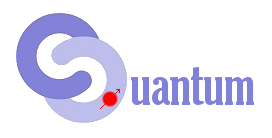
\includegraphics[scale=0.6]{pics/LogoIQC.png} &
\vspace{-2pt}

\includegraphics[scale=0.22]{pics/cs.png}
\end{tabular}

\vspace{68.5pt}
{\Huge #2}\\                           % diploma project text
\vspace{40pt}
{\Large #3}\\ \vspace{25pt}  % project title
{\Large #4}\\                          % project subtitle
\vspace{40pt}
{\LARGE \Name}\\                   % student name
\end{center}
\vspace{60pt}
\begin{tabular*}{\textwidth}{@{\extracolsep{\fill}}p{6cm}r}
&{\large\textbf{#5}}\vspace{10pt}\\      % scientific advisor
&{\large \Advisor}                                    % advisor name
\end{tabular*}
\vspace{20pt}
\begin{center}
{\large\textbf{#6}}\\                                % bucharest
\vspace{0pt}
{\normalsize \Year}
\end{center}
\end{titlepage}
}

\newcommand{\frontPageEN}{\frontPage{\UniTextEN}{\DiplomaEN}{\ProjectTitleEN}{\ProjectSubtitleEN}{\AdvisorEN}{\BucEN}}

\linespread{1.1}
\setlength\parindent{0pt}
\setlength\parskip{.23cm}

%% Abstract macro
\newcommand{\AbstractPageEN}{
\begin{titlepage}
\vspace*{-70pt}
{\large \textbf{ABSTRACT}}\vspace{10pt}\\
\AbstractEN \vfill
\end{titlepage}
}

\newcommand{\AbstractPageRO}{
\begin{titlepage}
\vspace*{-70pt}
{\large \textbf{ABSTRACT}}\vspace{10pt}\\
\AbstractRO \vfill
\end{titlepage}
}

%% Thank you macro
\newcommand{\ThanksPage}{
\begin{titlepage}
\vspace*{-70pt}
{\large \textbf{ACKNOWLEDGEMENTS}}\vspace{10pt}\\
\Thanks \vfill
\end{titlepage}
}



%%%%%%%%%%%%%%%%%%%%%%%%%%%%%%%%%%%%%%%%%%%%%%%%%%   
%%
%%          End of template definitions
%%   
%%%%%%%%%%%%%%%%%%%%%%%%%%%%%%%%%%%%%%%%%%%%%%%%%%


%%% Puteți elimina aceste linii din lucrare, servesc numai pentru template.
\newcommand{\worktype}[1]{[\textit{#1}] }
\newcommand{\dezvoltare}{\worktype{Dezvoltare de produs}}
\newcommand{\cercetare}{\worktype{Cercetare}}
\newcommand{\ambele}{\worktype{Ambele}}
%%%


%%
%%   Campurile de mai jos trebuie modificate de autor. Modificati doar continutul, nu si numele fiecarei definitii
%%
\newcommand{\ProjectTitleEN}{A comprehensive study on Integrating Quantum Physics in Deep Learning Networks for Optimizations in Computer Vision and Natural Language Processing Fields}
\newcommand{\ProjectSubtitleEN}{QRKT-GAN: Neural Ordinary Differential Equation-Inspired Generative Adversarial Network with Numerical Runge-Kutta Methods for Quantum Visual Transformer-Based Generator and Discriminator}
\newcommand{\Name}{Cătălin-Alexandru Rîpanu}
\newcommand{\Advisor}{Șl. dr. ing. Dumitru-Clementin Cercel}
\newcommand{\Year}{2024}

% Setări document
\title{Diploma Project}
\author{\Name}
\date{\Year}

%%
%%   Campurile aferente rezumatului
%%

\newcommand{\AbstractRO}{Modelele de Învățare Profundă, cum ar fi Rețelele Adversariale Generative (GAN-uri)~\cite{goodfellow2014generative} și Transformers Vizuali (ViTs)~\cite{vaswani2017attention, dosovitskiy2020}, au demonstrat rezultate remarcabile în diverse domenii ale Învățării Automate și Inteligenței Artificiale, inclusiv Clasificarea Obiectelor, Segmentarea Imaginilor, Analiza Sentimentelor și Generarea de Date Sintetice. Aceste rețele neuronale sunt esențiale în avansarea sistemelor care necesită precizie înaltă și o înțelegere profundă a datelor complexe într-o varietate de sarcini, atât în Procesarea Limbajului Natural (NLP), cât și în Vederea Computațională (CV).

Totuși, eficacitatea modelelor de Învățare Profundă vine cu provocări semnificative: acestea necesită un număr mare~\cite{chen2014big} de parametri pentru a învăța și a extrage caracteristici semnificative din datele reale. În plus, aceste rețele neuronale au nevoie de cantități vaste de informații pentru a atinge nivelurile de performanță dorite. Obținerea unor astfel de seturi mari de date poate fi dificilă, deoarece datele reale nu sunt adesea disponibile public și pot fi greu de colectat și filtrat. Acest lucru duce la cerințe semnificative de resurse computaționale atât pentru antrenare, cât și pentru optimizarea hiperparametrilor, adesea realizate prin tehnici exhaustive cum ar fi grid search~\cite{liashchynskyi2019grid}.

Pentru a aborda aceste provocări și pentru a investiga mai departe această direcție, această teză propune o arhitectură hibridă nouă de Rețea Generativă Adversarială care utilizează Transformers Vizuali Cuantici (QViTs)~\cite{di2022dawn} atât ca Generatori, cât și ca Discriminatori. Visual Transfomers sunt selectate pentru abilitatea lor superioară de a gestiona reprezentările de date complexe. O inovație cheie în această arhitectură este integrarea metodelor numerice ce rezolvă Ecuații Diferențiale Ordinare (ODE)~\cite{fan2024Quantum} ca Encoders ~\cite{hinton2011transforming}, îmbunătățind capacitatea modelului de a captura dinamica temporală și structurile complexe, și îmbunătățind conexiunile reziduale din cadrul arhitecturii Transformer-ului pentru a atenua și mai mult problema vanishing gradients~\cite{liu2020understanding}.

Mai mult, această arhitectură încorporează Circuite Variaționale Cuantice~\cite{cerezo2021variational} atât în Mecanismele de Auto-Atenție~\cite{voita2019analyzing}, cât și în Perceptronii Multistrat (MLPs)~\cite{popescu2009multilayer} ai Visual Transformers. Prin valorificarea principiilor Fizicii Cuantice, în special Mecanica, aceste circuite cuantice~\cite{benedetti2019parameterized} pot efectua operații algebrice complexe mai eficient decât metodele clasice, oferind un avantaj computațional semnificativ.

Performanța acestei abordări hibride este evaluată în raport cu o metodă de bază neurală pur clasică din literatură, folosind seturi de date din domeniile CV și NLP. Mai specific, configurațiile ODE cuantice sunt testate pe seturile de date CIFAR-10~\cite{Krizhevsky09learningmultiple}, MNIST~\cite{lecun2010mnist} și IMDb Reviews~\cite{maas-EtAl:2011:ACL-HLT2011}. Aceste arhitecturi de rețele neuronale sunt antrenate și testate eficient utilizând simulări numerice adaptate pentru Circuitele Variaționale Cuantice~\cite{Zhang_2023}. Rezultatele obținute indică faptul că aceste abordări hibride obțin performanțe comparabile de clasificare și generare cu metodele de bază clasice, în timp ce necesită mai puțini parametri antrenabili.

În plus, numărul redus de parametri în aceste modele hibride deschide posibilitatea rulării acestora pe dispozitive cuantice din era NISQ pentru antrenare și inferență. Această fezabilitate este un progres semnificativ, deoarece implică faptul că modelele îmbunătățite cuantice pot fi antrenate și implementate pe calculatoare cuantice reale, care sunt în prezent limitate în termeni de număr de qubiți și fidelitate operațională~\cite{lau2022nisq}.

Această teză demonstrează potențialul integrării Calculului Cuantic~\cite{nielsen2001quantum}, în special Mecanica Cuantică, cu arhitecturi avansate de Învățare Profundă pentru a crea rețele eficiente~\cite{huang2021power}.}

\newcommand{\AbstractEN}{Deep Learning models, such as Generative Adversarial Networks (GANs)~\cite{goodfellow2014generative} and Visual Transformers (ViTs)~\cite{vaswani2017attention, dosovitskiy2020}, have demonstrated remarkable results across various domains in Machine Learning and Artificial Intelligence, including Object Classification, Image Segmentation, Sentiment Analysis, and Synthetic Data Generation. These neural networks are pivotal in advancing systems that require high precision and a deep understanding of complex data across diverse applications within NLP(Natural Language Processing) and CV (Computer Vision).

However, the effectiveness of Deep Learning models comes with significant challenges: they require an extensive~\cite{chen2014big} number of parameters to learn and extract meaningful features from real-world data. Additionally, these neural networks need vast amounts of information to achieve desired performance levels. Obtaining such large sets can be difficult as real-world data is often not publicly available and can be challenging to collect and curate. This results in substantial computational resource requirements for both training and hyperparameter optimization, often achieved through exhaustive techniques such as grid search~\cite{liashchynskyi2019grid}.

To address these challenges and to further investigate this direction, this thesis proposes a novel hybrid Generative Adversarial Network architecture that employs Quantum Visual Transformers (QViTs)~\cite{di2022dawn} as both the Generator and Discriminator. Visual Transformers are selected for their superior ability to manage intricate data representations. A key innovation in this architecture is the integration of Ordinary Differential Equation (ODE)~\cite{fan2024Quantum} solvers as Encoders~\cite{hinton2011transforming}, enhancing the model capability to capture temporal dynamics and complex data structures, and improving the residual connections within the transformer architecture to mitigate the vanishing gradients problem~\cite{liu2020understanding} even more.

Moreover, this architecture incorporates VQCs (Variational Quantum Circuits)~\cite{cerezo2021variational} in MSA (Multihead Self-Attention)~\cite{voita2019analyzing} and FFNs (Feed-Forward networks)~\cite{popescu2009multilayer}, all of them being integrated in Visual Transformers. By leveraging the principles of Quantum Physics, especially Mechanics, these quantum circuits~\cite{benedetti2019parameterized} can perform complex algebraic operations more efficiently than classical methods, offering a significant computational advantage.

The performance of this hybrid approach is benchmarked against a purely classical neural network baseline from the literature using datasets from both CV and NLP areas. Specifically, the Quantum ODE configurations are tested on CIFAR-10~\cite{Krizhevsky09learningmultiple}, MNIST~\cite{lecun2010mnist} and IMDb Reviews~\cite{maas-EtAl:2011:ACL-HLT2011} datasets. These neural network architectures are effectively trained and tested using numerical simulations tailored to Variational Quantum Circuits~\cite{Zhang_2023}. The obtained results indicate that these hybrid approaches achieves comparable classification and generation performance to the classical baseline, while requiring fewer trainable parameters.

Furthermore, the reduced parameter count in these hybrid models opens up the possibility of running it on Noisy Intermediate-Scale (NISQ) quantum devices for both training and inference. This feasibility is a significant breakthrough, as it implies that quantum-enhanced models can be trained and deployed on actual quantum computers, which are currently limited in terms of the number of qubits and operational fidelity~\cite{lau2022nisq}.

This thesis demonstrates the potential of integrating Quantum Computing~\cite{nielsen2001quantum}, especially Quantum Mechanics, with advanced Deep Learning architectures to create more efficient and powerful networks which can significantly reduce computational costs while maintaining high performance, paving the way for more scalable and effective AI applications~\cite{huang2021power}.}

%%
%%   Campurile aferente paginii de multumiri
%%
\newcommand{\Thanks}{
First and foremost, I would like to express my deepest gratitude to my advisor, Prof. Dumitru-Clementin Cercel, for his unwavering support and insightful guidance throughout my research journey. His expertise and encouragement have been essential in exploring the intricate intersection of Machine Learning and Quantum Mechanics, widely referred to in the literature as Quantum Machine Learning. This interdisciplinary field, though initially daunting, is at the cutting edge of technological advancement and innovation in both areas.

I am also profoundly thankful to Prof. Pantelimon-George Popescu for his advice, recommendations, and exceptional lectures on Quantum Computing. His mentorship has been instrumental in building a robust understanding of this groundbreaking paradigm, which promises new solutions to problems previously deemed insurmountable by classical methods.

Furthermore, I wish to acknowledge the significant contributions of the academic teaching assistants and collaborators encountered during my bachelor's studies. Their guidance during challenging times has been crucial to my academic development. Last but not least, I am also grateful for the computational resources provided by the Computer Science and Engineering Department, which were essential for the design and implementation of this project.

In addition, I extend my appreciation to my friends for their continuous support, ideas, and advice, especially during moments when inspiration was scarce. Lastly, my heartfelt thanks go to my parents for their enduring sacrifices and unwavering support throughout this journey into the unknown. Their belief in me has been a constant source of motivation.
}

\makeatletter
\def\@makechapterhead#1{%
  \vspace*{-55\p@}%
  {\parindent \z@ \raggedright \normalfont
  \ifnum \c@secnumdepth >\m@ne
  \Large\bfseries \thechapter\space% Adjust the size as needed
  \fi
  \interlinepenalty\@M
  \Large \bfseries #1\par\nobreak
  \vskip 12\p@
  }}
  
\makeatother

\begin{document}

\setcounter{page}{1}
\frontPageEN


\setcounter{page}{2}
\ThanksPage \pagestyle{fancy}

\AbstractPageEN\pagestyle{fancy}

\AbstractPageRO\pagestyle{fancy}

\renewcommand{\contentsname}{\vspace{-3.45cm} CONTENTS}
\tableofcontents
% Textul licentei incepe de aici 

\chapter{Introduction}\pagestyle{fancy}

\section{Context}\vspace{-12pt}\label{context}
Artificial Intelligence models, particularly Deep Learning ones, have made significant contributions to solving real-world tasks, greatly improving human lives in various fields, such as Medical Image Recognition~\cite{he2020infusing}. Despite their impressive capabilities, Deep Learning models come with substantial drawbacks regarding computational resources~\cite{chen2014big} and effort. Achieving high performance with these models necessitates learning millions to billions of parameters, also called weights or artificial neurons, which demands considerable resources and preparation time. This limitation also has negative environmental impacts due to high power consumption.

Over the years, researchers have developed numerous solutions to mitigate the problem of minimizing the number of parameters using interesting classical algorithms and techniques. These include, for example, specialized activation functions for neural layers like Rectified Linear Unit~\cite{NIPS2017_a96b65a7}, Leaky ReLU~\cite{xu2020reluplex}, Gaussian Error Linear Unit~\cite{hendrycks2016gaussian}, Softmax~\cite{liu2016large}, Sigmoid~\cite{han1995influence} and Hyperbolic Tangent~\cite{zamanlooy2013efficient}. Additionally, effective optimizers such as AdamW~\cite{zhang2018improved} and Stochastic Gradient Descent~\cite{bottou2010large} have been utilized to combat this limitation, along with methods like Learning Rate Schedulers~\cite{wen2021convolutional}, Weight Decay~\cite{loshchilov2017decoupled}, and Dropout~\cite{srivastava2014dropout} to reduce also the chances of model overfitting. Over the years, various architectural designs and network combinations have emerged to address these challenges. However, the tradeoff between high computational resource consumption and performance remains a difficult issue, especially when scaling up the dimensions of available noisy real-world datasets used for training. It is unlikely\footnote{\url{https://www.theverge.com/24066646/ai-electricity-energy-watts-generative-consumption}} to be efficiently resolved in the near future using solely classical approaches.

A segment of Computer Science researchers, in collaboration with physicists, have taken a bold and innovative approach to these challenges by exploring solutions from a physical perspective, leading to the emergence of Quantum Computation and Quantum Information~\cite{nielsen2001quantum}. Leveraging the principles of Quantum Mechanics, AI research has begun to explore Deep Learning optimizations using quantum facilities, such as Variational Quantum Circuits~\cite{benedetti2019parameterized} or Quantum Algorithms~\cite{cerezo2021variational}, to develop hybrid Deep Learning models. By combining classical and quantum methodologies, new experiments can be conducted to address performance and resource demands more efficiently, thus utilizing the unique capabilities of quantum hardware. This involves training these models on it, also known as Parameterized Quantum Circuits~\cite{benedetti2019parameterized}, where the parameters are referred to as the qurons of the quantum model.

Quantum Computing leverages properties like superposition~\cite{koprinkov2023quantum} and entanglement~\cite{Horodecki_2009}, enabling the execution of complex algebraic operations that are infeasible for classical computers. QA (Quantum Algorithms)~\cite{cerezo2021variational}, like Grover's Algorithm~\cite{shi2017coherence}, QPE~\cite{o2019quantum}, QFT~\cite{weinstein2001implementation} and Deutsch-Jozsa Quantum Parallelism~\cite{gulde2003implementation}, provide exponential speedups for certain tasks. Integrating these Quantum principles with Deep Learning can significantly reduce the number of parameters and computational resources required while maintaining or even enhancing model performance. This interdisciplinary distinctive approach, also known as Quantum Machine Learning, opens up exciting possibilities for the future of AI, promising advancements that could transform how complex problems are approached and solved in ways that classical computers, with their current architecture, could never achieve.
\section{Problem}\vspace{-12pt}
Over the years, numerous algorithms, techniques, network architectures, and methodologies have been proposed in Deep Learning to tackle a many tasks, such as Object Classification, Synthetic Data Generation and Detection, in NLP, CV, Domain Adaptation~\cite{farahani2020brief} and Knowledge Distillation~\cite{hinton2015distilling}. These approaches have achieved high performance metrics like Accuracy, AUC, ROC, and F1 scores. The advent of High Performance Computing (HPC) facilities, particularly classical parallelism, has enabled Deep Learning models to process billions of examples from noisy real-world datasets effectively, thus yielding impressive results.

Despite these advancements, a significant drawback persists: the enormous number of neurons and the corresponding computational resources required by these models. Traditional solutions in classical Deep Learning, such as Cross Validation~\cite{berrar2019cross}, RS(Random Search)~\cite{liashchynskyi2019grid}, GS(Grid Search)~\cite{liashchynskyi2019grid}~\cite{liashchynskyi2019grid} and Keras Tuner~\cite{pon2021hyperparameter} are commonly employed, together with Layer Augmentation until model performance plateaus or overfits. To also mitigate overfitting, regularization techniques such as Ridge, Lasso, Elastic-Net~\cite{ogutu2012genomic} or Dropout~\cite{srivastava2014dropout} can be applied. However, these methods often involve exhaustive hyperparameter searches, which are extremely time-consuming, especially when dealing with validation sets comprising billions of data points for complex tasks. Group sparsity regularizers can also be applied to network parameters, where each group acts on a single neuron, thus reducing the neurons while maintaining the model score~\cite{alvarez2018learning}.

Another method employed to address these challenges is Transfer Learning~\cite{weiss2016survey}, which involves locating and initializing a pretrained model to use as a baseline before refining it with a targeted dataset. This approach can help achieve good performance with less effort on architecture design and expedite the training process. However, the availability of suitable pretrained models is limited, and fine-tuning may yield only decent, if not disappointing, results, due to differences in the data distributions between the pretraining and fine-tuning datasets.

The primary challenge lies in balancing time, memory and power consumption on classical systems to make robust and valid neural architectural choices. Furthermore, reducing the number of neurons too drastically is not a solution as it can lead to underfitting and degraded performance, making it difficult to solve complex and challenging tasks with decent results. The iterative process of tuning hyperparameters and optimizing model architectures is computationally intensive and often results in a significant trade-off between resource consumption and model performance~\cite{liashchynskyi2019grid}.

Moreover, the reliance on vast amounts of training data for achieving desired performance further exacerbates these issues. Real-world datasets are often difficult to obtain and may not be publicly available, which complicates the development and fine-tuning of effective Deep Learning models. The extensive time and computational costs associated with hyperparameter optimization and model training present significant obstacles to advancing AI capabilities while maintaining efficiency and sustainability. This trade-off between computational resource consumption and performance remains a persistent and challenging problem in the field of Deep Learning, highlighting the need for innovative solutions that can overcome these limitations.

\section{Objective}\vspace{-12pt}
In the current landscape of Deep Learning research, there is an ongoing investigation into whether integrating models into a purely quantum environment can significantly reduce power consumption and the number of trainable parameters without sacrificing performance. This exploration leverages techniques such as the Ansatz~\cite{hadfield2019Quantum} and Variational Quantum Circuits~\cite{cerezo2021variational}. As classical supercomputers advance to handle increasingly complex deep models, their power consumption grows almost exponentially. In contrast, quantum machines exhibit an exponential increase in computational power while maintaining a linear increase in power consumption. This intriguing characteristic makes a strong case for Quantum Computing: with the advent of fault-tolerant quantum computers, qubits could serve as highly efficient artificial neurons in neural networks. Quantum-inspired techniques could enable networks to operate with a vast number of neurons per layer at minimal energy cost, dramatically reducing overall energy consumption\footnote{\url{https://www.eetimes.eu/how-Quantum-Computing-can-help-make-ai-greener}}.

Building on the challenges outlined in the above section, the primary goal of this thesis is to explore Deep Learning models, both pure Quantum and hybrid, that leverage neural ODE-based architectures~\cite{zhong2022neural} inspired by non-trivial Variational Quantum Circuits~\cite{cerezo2021variational} within the context of Visual Transformers~\cite{vaswani2017attention, dosovitskiy2020} and their complex Encoders~\cite{hinton2011transforming} and Decoders~\cite{breuckmann2018scalable}. The most important objective is to minimize the number of parameters used by deep network layers utilizing the idea~\cite{Comajoan_Cara_2024} of replacing traditional linear transformation layers in MHA~\cite{voita2019analyzing} and Multi-Layer Perceptrons~\cite{popescu2009multilayer} with Quantum Circuits~\cite{benedetti2019parameterized}. Additionally, low truncation error Neural Ordinary Differential Equation~\cite{zhong2022neural}\cite{li2022ode} techniques will be employed to further optimize Transformer Layers, namely Runge-Kutta Methods~\cite{butcher1996history} of 1st, 2nd, 3rd, and 4th order. An analysis of Runge-Kutta 4th order method optimization which is not theoretically grounded in standard RK methods, but in terms of training, will also be included~\cite{li2022ode}.

To better understand the rationale and motivation behind the proposed Deep Learning model in this paper, it is necessary to compare these Quantum ODE-based Transformers configurations  with their classical counterparts using the datasets mentioned in Abstract. The network utilizing the optimized Runge-Kutta 4th order method will be leveraged within the context of Vision Transformers (ViTs)~\cite{vaswani2017attention, dosovitskiy2020} and integrated into a Generative Adversarial Network (GAN)~\cite{goodfellow2014generative} architecture. In this configuration, both the Generator and Discriminator will be Quantum Visual Transformers (QViTs)\footnote{\url{https://openreview.net/pdf?id=p7xPXoKB0H}}, incorporating the optimized Neural ODE solver to generate realistic and informative synthetic data without being limited to specific types of distributions. This will be achieved using techniques such as Data Augmentation~\cite{zhao2020diffaugment} and Image Recognition at Scale~\cite{dosovitskiy2020} in the context of ViTs.

The final proposed architecture in this thesis, named QRKT-GAN, will be tested on a real-world consistent dataset, namely CIFAR-10~\cite{Krizhevsky09learningmultiple}, and compared using the same data with a renowned classical counterpart, TransGAN~\cite{jiang2021transgan}, which is a strong architecture built entirely free of Convolutions~\cite{cordonnier2020relationship}. These comparative analysis and results will provide another argument for the possible advantages of integrating Quantum Computing~\cite{nielsen2001quantum} with advanced Deep Learning neural networks under the right context.
\section{Paper Structure}\vspace{-12pt}
The next chapter delves into the most relevant and important classical and Variational Quantum Algorithms~\cite{cerezo2021variational} and techniques developed over the years to leverage both Quantum and hybrid logic in Deep Learning for model optimization. This chapter will illustrate how these both hybrid and pure Quantum Neural Networks (QNNs)~\cite{breuckmann2018scalable} are designed to be compatible with Noisy Intermediate-Scale (NISQ)~\cite{lau2022nisq} devices provided by specialized vendors such as IBM~\cite{Santos_2016}, Google~\cite{kalai2023googles}, Microsoft~\cite{Mykhailova_2023}, and Amazon~\cite{Reyes_2021}. It will explore the advancements that make it possible to run complex Deep Learning models on quantum computers, highlighting the interplay between Quantum Computing~\cite{nielsen2001quantum} and Deep Learning for neural depth decreasing while not losing too much performance.

Section three will discuss the foundational concepts of Machine Learning, Deep Learning and Ordinary Differential Equations. It will also provide a comprehensive overview of Quantum Computation and Quantum Information~\cite{nielsen2001quantum}, and will also introduce the emerging field of Quantum Machine Learning~\cite{dunjko2018machine}. This section aims to explain how quantum principles can enhance the capabilities of Deep Learning solutions in addressing high-demanding tasks, some of which are classified as NP-Hard~\cite{chatterjee2024solving} or NP-Complete~\cite{furer2008solving}. By understanding these fundamentals, the reader will gain insight into the potential synergies between Classical and Quantum Computing~\cite{nielsen2001quantum}, which together can form a duality in the world of Artificial Intelligence.

Section four will present an in-depth analysis of the proposed Ordinary Differential Equation-based Quantum Neural Networks (QNNs)~\cite{abbas2021power, li2022ode} configurations. This includes their motivation, underlying concepts, mathematical and quantum frameworks, but also their physical limitations, and future potential within their problem domain environment. The chapter will also discuss in-detail the new ODE-based GAN architecture in detail, QRKT-GAN, explaining how it incorporates the traversed knowledge to minimize the solution of the optimization problem outlined in \ref{context} section, while maintaining acceptable performance in Synthetic Image Generation.

The fifth chapter will detail the methodologies adopted for conducting the experiments. This includes a comprehensive description of the datasets used, their internal characteristics, and the reasons for their selection. It will compare various Quantum ODE-based~\cite{fan2024Quantum} configurations with their classical ODE-based networks~\cite{zhong2022neural} counterparts to fully understand the benefits and limitations of quantum-enhanced models. Additionally, the chapter will provide a detailed comparison between the proposed QRKT-GAN model and its classical baseline, TransGAN~\cite{jiang2021transgan}, using the CIFAR-10~\cite{Krizhevsky09learningmultiple} dataset. This analysis will highlight the benefits and challenges of integrating Quantum Computing into Deep Learning, presenting it as a viable alternative solution for very specific optimization problems.

The final chapter will summarize the main ideas presented in the thesis, highlighting the relevance of the results and drawing key conclusions. It will also propose future work and outline potential directions for additional exploration in the realm of Quantum Deep models studies, focusing on power consumption, computational resources and performance optimization. This chapter will emphasize the importance of continued exploration in combining Quantum Computing with Machine Learning~\cite{dunjko2018machine} to achieve more efficient and powerful neural solutions.

\chapter{Related Work}\vspace{-12pt}
The relentless demand for improving human lives continues unabated, with increasingly complex and data-intensive needs emerging. This necessitates the development of sophisticated models capable of delivering accurate and reliable results. However, the complexity and depth of these models often result in significantly high computational resource consumption, which has environmental implications due to the energy required for such intensive processing.

Over the years, numerous classical, quantum, and hybrid methods have been proposed to address the optimization problem of minimizing model depth without significantly sacrificing performance. One notable approach is real-time learning of the number of neurons in deep networks using structured sparsity during training, which dynamically adjusts the network structure to optimize performance without excessive resource use~\cite{alvarez2018learning}. Another method involves crafting specialized architectures that maintain a constant computational budget while slightly increasing depth to improve performance. This is achieved by dimensionality reduction before applying expensive Convolutions~\cite{wen2021convolutional} with larger patch sizes~\cite{Szegedy_2015_CVPR}. Unfortunately, Convolutions~\cite{wen2021convolutional} have been shown~\cite{cordonnier2020relationship} to be less effective in capturing global feature interactions, as they primarily focus on local patterns in data processing. In contrast, the Self-Attention mechanism~\cite{voita2019analyzing} utilized in Transformers~\cite{vaswani2017attention} excels at capturing these global interactions.

In addition, some techniques focus on minimizing weights during training by splitting network weights into sets or hierarchies of multiple groups, each using disjoint sets of features. This allows parallelization, even in an embarrassingly manner, as each subnetwork operates independently, enhancing computational efficiency~\cite{pmlr-v70-kim17b}. Alternatively, population-based heuristic algorithms, such as Particle Swarm Optimization (PSO), have shown promise in optimally determining the number of parameters without exhaustive searches like grid search~\cite{liashchynskyi2019grid}, thereby conserving valuable computational resources during the fine-tuning process of these DL networks~\cite{7986470}.

An alternative strategy entails minimizing the number of model parameters in deep neural networks by employing product-of-sums matrix decomposition techniques, which decompose linear operators expressed as a product of sums of more basic linear operators~\cite{wu2018prodsumnet}. For Convolutional Neural Network~\cite{wen2021convolutional} models, kernel-sharing between multiple convolutional layers can also be applied~\cite{azadbakht2022drastically}. Kernel-sharing is possible exclusively between layers that share the same kernel dimensions, as well as identical input and output channels.

Despite their advantages, these classical methods have inherent drawbacks. Designing neural architectures from scratch to meet specific requirements is challenging and time-consuming. Moreover, methods like Particle Swarm Optimization~\cite{7986470} require optimization of extra aspects, like activations~\cite{han1995influence, NIPS2017_a96b65a7, xu2020reluplex} or setting the number of entire dataset iterations (epochs) to be truly effective. Quantum Neural Networks (QNNs)~\cite{abbas2021power} and Quantum Algorithms~\cite{cerezo2021variational} offer new avenues for addressing these limitations, providing potential solutions for power-efficient Deep Learning. Various Quantum frameworks, technologies, GPU-based numerical simulators, and access to real hardware have been developed to facilitate the implementation of quantum phenomena in Machine Learning.

However, the quantum approach shares a common challenge with classical methods: the need for specific adaptations for each type of Deep Learning model.
In the classical domain, the entire architectural framework must be analyzed to prevent performance degradation.
\chapter{Background}\vspace{-12pt}
This chapter will delve into the main and most important advancements in Machine Learning, presenting key concepts as they appeared in the literature. It will discuss the motivation and necessity of Deep Learning, a fundamental subdomain of Machine Learning, to fully understand the creation and utilization of neural networks. This will include an exploration of why Generative Adversarial Networks (GANs)~\cite{goodfellow2014generative} and Visual Transformers~\cite{vaswani2017attention, dosovitskiy2020} were developed, along with a detailed examination of their architectural specificities and functions.

Furthermore, the chapter will provide an overview of the techniques used to identify optimal hyperparameters, which are crucial for further neural model optimization. This will cover various approaches to fine-tuning Deep Learning models to enhance their performance.

A significant portion will be dedicated to Ordinary Differential Equations (ODEs) and their most popular numerical solvers, highlighting the foundational aspects of the Runge-Kutta methods~\cite{butcher1996history}. It will explain how to interpret Transformer layers from an ODE perspective~\cite{li2022ode}, providing a mathematical framework for understanding these non-trivial neural network structures.

Furthermore, a concise summary of Quantum Computing~\cite{nielsen2001quantum} will also be presented, establishing the prerequisites for understanding Quantum Machine Learning~\cite{dunjko2018machine}. This section will articulate the motivation behind integrating Runge-Kutta ODE methods~\cite{butcher1996history, fan2024Quantum} into Quantum Computing~\cite{nielsen2001quantum}. By exploring carefully Quantum Gates and Circuits~\cite{barenco1995elementary, benedetti2019parameterized}, Variational Quantum Algorithms and Circuits~\cite{cerezo2021variational, benedetti2019parameterized}, their motivation and application in the context of Quantum Transformers~\cite{Comajoan_Cara_2024} will be illustrated.

By comprehensively covering these topics, the chapter aims to equip readers with a deep understanding of the theoretical and practical foundations necessary for advancing in the field of Quantum Machine Learning~\cite{dunjko2018machine}, particularly through the integration of ODE methods~\cite{zhong2022neural} in quantum frameworks~\cite{Zhang_2023}.

\section{ML (Machine Learning)}\vspace{-12pt}
ML is the practice of empowering computers to acquire knowledge from data and make decisions without being explicitly programmed to do so. A crucial aspect of Machine Learning is training models on data before they can autonomously make decisions. Thus, data is fundamental to Machine Learning algorithms. Without data, Machine Learning cannot function, as models rely entirely on the information provided to make future predictions. The data used must accurately reflect real-world scenarios because Machine Learning models depend on this data to learn and generate accurate predictions for new, unseen data~\cite{machinelearning}.

In practice, Machine Learning involves extensive mathematical operations such as matrix multiplication, feature scaling, and normalization. Consequently, the data fed into Machine Learning algorithms must be represented as numerical vectors or numbers, as opposed to text or other non-numerical forms that machines cannot directly interpret.

For instance, textual data and alphabets are not directly understandable by machines; hence, they must be converted into numerical form before being processed by Machine Learning models. Techniques such as one-hot encoding, word embeddings, or other numerical transformation methods are used to convert text into a machine-readable format, enabling models to learn from and predict based on the data provided.

Machine Learning algorithms, along with neural networks, have been proposed for many decades. However, during the early days, the lack of sufficient data and limited computational power hindered their practical application. Today, the scenario has drastically changed. Companies generate vast amounts of data, and computational resources have become extraordinarily powerful and accessible. Services (such as Microsoft, AWS, Google) provide scalable computational power, allowing users to run complex Machine Learning algorithms without the need for setting up their own hardware infrastructure. This has led to an exponential growth in the demand for applications in ML and DL~\cite{machinelearning}.

Understanding DL and ML is crucial in this data-rich environment. The ability to harness data through these technologies enables companies to make informed predictions, optimize processes, and drive innovation. The more effectively Machine Learning models are trained and utilized, the greater the value they can bring to an organization, ultimately contributing to increased profitability and competitive advantage.

Types of ML (Supervised Learning, Unsupervised Learning, Semi-Supervised Learning)~\cite{machinelearning}:
\begin{itemize}
  \item \textbf{SL}: This method trains a Machine Learning model on a dataset where the output labels are known. The model learns to map inputs to outputs based on this labeled data. During training, the model's predictions are compared with the actual labels to assess performance and adjust parameters. This process repeats until the model reaches a desired accuracy.
  \item \textbf{UL}: A common application is customer segmentation, where customers are grouped based on behaviors like purchase history or browsing patterns, without predefined labels. This helps businesses tailor their marketing strategies to different customer groups. This method involves training the model on data without labeled outputs.
  \item \textbf{SSL}: For instance, in text document classification, a model is initially trained on a subset of documents with known categories. It then classifies the remaining documents, which lack predefined labels, based on the learned patterns. This paradigm proves its usefulness in that moment when labeled data is scarce or costly to obtain.
\end{itemize}

\section{GD (Gradient Descent)}\vspace{-12pt}
GD is a fundamental 1st-order technique widely used in ML and DL for minimizing cost or loss functions. This iterative method works by iteratively adjusting the parameters in a network to find the local minimum or maximum of a given function, thereby improving the model accuracy. GD helps with difference between the real and obtained result minimization with the use of neurons updates. Its significance and simplicity make it a fundamental topic in nearly all introductory ML courses, as it provides a clear understanding of how models learn and improve from data~\cite{gradientdescent}.

The Gradient Descent algorithm is not universally applicable to all functions. For it to work effectively, the function must meet two specific criteria: it must be differentiable and convex.

Mathematically:
\begin{itemize}
  \item A function is differentiable if it has a derivative at each point in its domain. This means the function must be smooth and continuous without any sharp corners or discontinuities. Differentiability is crucial because GD relies on the gradient (the derivative) to determine the direction and stride magnitude to take towards the maximum and minimum . If it is not differentiable, the algorithm cannot compute the gradient accurately, leading to unreliable optimization results.
        \begin{figure}[th]
          \centering
          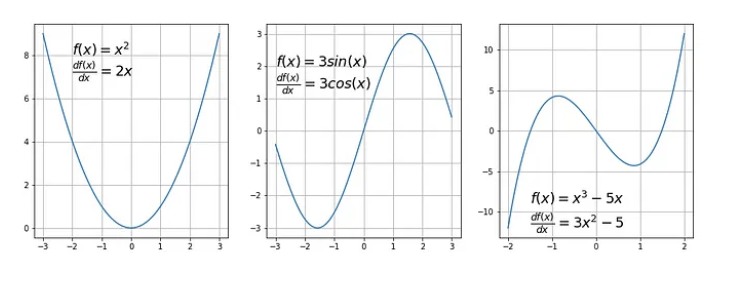
\includegraphics[scale=0.637]{./pics/diff_func.png}
          \caption[Examples of differentiable functions]{Examples of differentiable functions. Image from~\cite{gradientdescent}.}
          \label{fig:pic1}
        \end{figure}
        \begin{figure}[th]
          \centering
          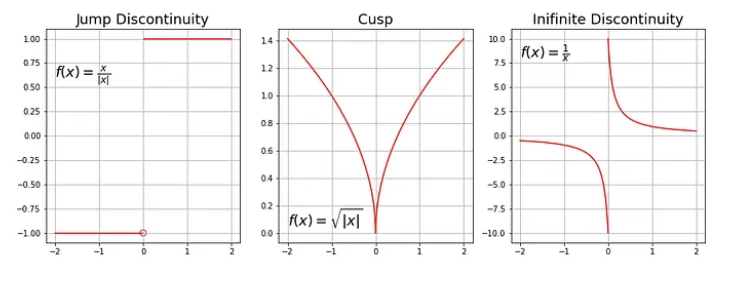
\includegraphics[scale=0.637]{./pics/undiff_func.png}
          \caption[Examples of non-differentiable functions]{Examples of non-differentiable functions~\cite{gradientdescent}.}
          \label{fig:pic2}
        \end{figure}
  \item A procedure is said to be convex if for any \( x_1 \) and \( x_2 \) in its domain, and for all \( \lambda \) in \([0, 1]\), this statement is true:
        \begin{equation}
          f(x_2) + \lambda f(x_1) - \lambda f(x_2) \geq f(x_2 - \lambda x_2 + \lambda x_1)
        \end{equation}
        Convexity ensures that any local minimum is also a global minimum, making it easier for Gradient Descent to find the optimal solution.
        \begin{figure}[th]
          \centering
          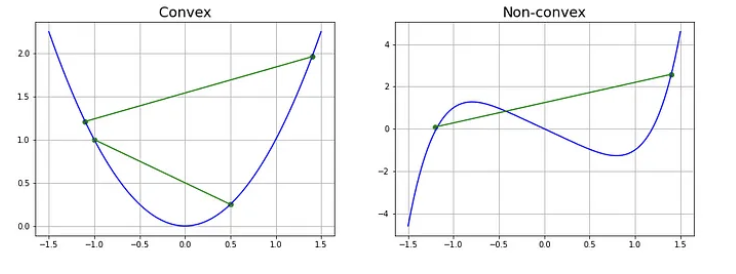
\includegraphics[scale=0.637]{./pics/conv_unconv_func.png}
          \caption[Examples of non-differentiable functions]{Examples of convex and non-convex functions~\cite{gradientdescent}.}
          \label{fig:pic3}
        \end{figure}
\end{itemize}


GD is a method for optimizing a procedure by iteratively heading in the direction that reduces it most sharply. In each iteration, it computes $\nabla(f)$, multiplies this gradient by a lr(learning rate), and adjusts the position by moving in the direction opposite. This approach ensures progression towards the function minimum:

\begin{equation}
  \mathbf{a}_{n} = \mathbf{a}_{n-1} - \eta \nabla f(\mathbf{a}_{n-1})
\end{equation}

where:
\begin{itemize}
  \item $\mathbf{a}_{n-1}$ is the location at the current moment of time.
  \item $\eta$ is lr.
  \item $\nabla f(\mathbf{a}_{n-1})$ is the multidimensional derivative of the procedure.
\end{itemize}

By repeatedly applying this update rule, GD shall converge. Furthermore, for maximizing the received procedure, the algorithm would instead add the scaled gradient~\cite{gradientdescent}.

In GD algorithms, the lr, represented by \(\eta\), is a key hyperparameter that dictates the step size taken at each iteration as the algorithm converges towards the min. of the loss function. The selection of the lr greatly influences the algorithm effectiveness:

\begin{itemize}
  \item \textbf{Small LR}: If it is too small, it will convergence very slowly, potentially requiring many iterations to reach the optimal point. In some cases, the algorithm may even hit the maximum number of iterations before converging.
  \item \textbf{Large LR}: If it is too large, sometimes it will not converge to the desired optimal point. Instead, it could overshoot the minimum, causing the algorithm to oscillate or even diverge entirely, failing to find a satisfactory solution.
\end{itemize}

Thus, selecting a good lr is essential for effective training of ML models~\cite{gradientdescent}.

\subsection{AdamW Optimizer}

Adam combines the strengths of both Stochastic Gradient Descent (SGD)~\cite{bottou2012stochastic} with Momentum and Root Mean Square Propagation (RMSProp). It computes the exp moving averages for both the gradient second and first moments. Like SGD with Momentum, it fully helps smooth out the updates to accelerate convergence. Similar to RMSProp, Adam uses adaptive learning rates for each parameter, allowing smaller steps for steep gradients and larger steps for flatter areas. Additionally, Adam adjusts these learning rates by considering both the mean of the first moment (the gradient) and the mean of the second moment (the squared gradient). The parameter improvement:~\footnote{\url{https://www.linkedin.com/pulse/understanding-adam-adamw-dsaisolutions-ileof/}}:
\begin{equation}
  w_{t+1} = w_t - \eta \frac{\hat{n}_t}{\sqrt{\hat{h}_t} + \epsilon}
\end{equation}
\begin{equation}
  n_t = \alpha_1 n_{t-1} + \nabla_\theta f(w_t) - \alpha_1\nabla_\theta f(w_t)
\end{equation}
\begin{equation}
  h_t = \alpha_2 h_{t-1} + (\nabla_\theta f(w_t))^2 - \alpha_2(\nabla_\theta f(w_t))^2
\end{equation}
Such as:

\begin{itemize}
  \item \(w\) is the parameter to be updated
  \item \(\eta\) is lr
  \item \(\alpha_1\) 1st moment decay, the default being 0.9
  \item \(\alpha_2\) 2nd moment decay, the default being 0.999
  \item \(\epsilon\) is a very small quantity used for preventing floating point exceptions
  \item \(\nabla_\theta f(\theta)\) is grad of the loss function \(f(w)\)
\end{itemize}

Exponentially smoothed avg of squared grads, \( h_t \), in the last equation, is sometimes referred to as the second moment or uncentered variance, due to the fact that the mean of the gradients is not subtracted. Additionally, \( n_t \) is often called the first moment or mean, representing the exponentially smoothed avg of grads, which captures cumulative history of grads. What is more, in Adam optimizer, the direction of the update is determined by normalizing the first moment with respect to the second moment~\cite{adamoptimizerw}.

Initially, the moving averages \( n_0 \) and \( h_0 \) are set to zero vectors. This initialization results in the moment approximations being skewed towards 0, particularly during the early stages, particularly when the decay rates \( \alpha_1 \) and \( \alpha_2 \) are near 1. To address the mentioned issue, training errors-corrected estimates \( \hat{m}_t \) and \( \hat{v}_t \) are calculated. This correction helps control the weights while approaching the global minimum, preventing high oscillations. The formulas for the bias corrections are as follows~\cite{adamoptimizerw}:

\begin{equation}
  \hat{n}_t = \frac{n_t}{1 - \alpha_1^t}
\end{equation}

\begin{equation}
  \hat{h}_t = \frac{h_t}{1 - \alpha_2^t}
\end{equation}

If no correction is applied, with \(\alpha_1 = 0.9\) and \(\alpha_2 = 0.999\), for the initial step, there are \(n_1 = 0.1 g_t\) and \(h_1 = 0.001 g_t^2\), causing the denominator in the update rule to become large. However, with bias-corrected estimates, the denominator becomes less sensitive to \(\alpha_1\) and \(\alpha_2\). The default values of \(\alpha_1\) and \(\alpha_2\) are set to 0.9 and 0.999, respectively, to retain as much historical gradient information as possible.

In practice, \(\alpha_2\) is usually set much closer to 1 than \(\alpha_1\), following the recommendation of the authors (\(\alpha_2 = 0.999\), \(\alpha_1 = 0.9\)). Consequently, the update coefficient \(1 - \alpha_2 = 0.001\) is significantly smaller than \(1 - 0.1 - \alpha_1 = 0\). By accounting for both the first and second moments when updating parameters, Adam improves optimization efficiency in very deep models with numerous neurons.


Nevertheless, Adam performance can be highly dependent on the initial hyperparameters and learning rate, leading to its convergence and stability negative modifications. Moreover, it may overfit, particularly with small datasets.

To address the generalization issue, Ilya Loshchilov and Frank Hutter introduced AdamW, an improved version of Adam, in their 2019 paper "Decoupled Weight Decay Regularization"~\footnote{\url{https://openreview.net/forum?id=Bkg6RiCqY7}}. Unlike Adam, AdamW effectively separates weight decay from the whole process in optimizations, thereby avoiding its implicit connection with the lr.

The separation allows the learning rate and weight decay to be optimized independently. As a result, adjusting the learning rate does not necessitate recalculating the optimal weight decay, leading to more stable and effective optimization.

\section{DL (Deep Learning)}
DL, a subset of ML, emphasizes algorithms based on the neural networks structure and function in the human brain. Unlike traditional Machine Learning algorithms that often require manual feature extraction and rely on simpler linear or non-linear models, Deep Learning employs complex architectures known as Artificial Neural Networks (ANNs). These neural networks are designed to automatically and hierarchically extract features from unprepared data, constructing them especially potent for handling tasks that involve extensive and unorganized bases of data.

Deep Learning models, particularly those involving DNNs (Deep Neural Networks), comprise multiple layers of interconnected learnable parameters. Every trainable parameter in a layer processes input data, applies a transformation using weights and biases, and passes the output to the next layer. The hierarchical nature of these layers allows Deep Learning models to learn increasingly abstract and complex representations of the data as it moves through the network. This capability empowers DL neural networks to excel in tasks like Speech and Image Identification, Natural Language Processing, and Game Playing.

One of the primary good property of DL is its capability to train from vast amounts of data without the use for extensive handcrafted attributes engineering. For instance, in Image Recognition tasks, traditional Machine Learning approaches might require handcrafted features such as edges, textures, and shapes. In contrast, DL neural network models have the possibility to be trained to detect these attributes directly from the pixel information~\cite{deeplearning}.

DL has achieved remarkable success across various domains, driven by advancements in computational power (especially GPUs), large datasets, and novel neural architectures such as RNNs (Recurrent Neural Networks), CNNs (Convolutional Neural Networks) and Transformers~\cite{vaswani2017attention}. CNNs, for example, are particularly highly suitable for tasks involving images, while Transformers~\cite{vaswani2017attention} and RNNs perform good in Data Manipulation which is in sequential form, such as Language Modeling and Translation.
\subsection{Artificial Neural Networks (ANN)}
An artificial neural network (ANN) consists of interconnected units, also referred to as artificial neurons(parameters) or units, arranged into many layers. These layers include the input data layer, one or more hidden data layers, and the output datat layer. Because of the numerous layers, ANNs are also called, sometimes, deep neural networks when there are many hidden data layers~\cite{ann}.

\begin{figure}[th]
  \centering
  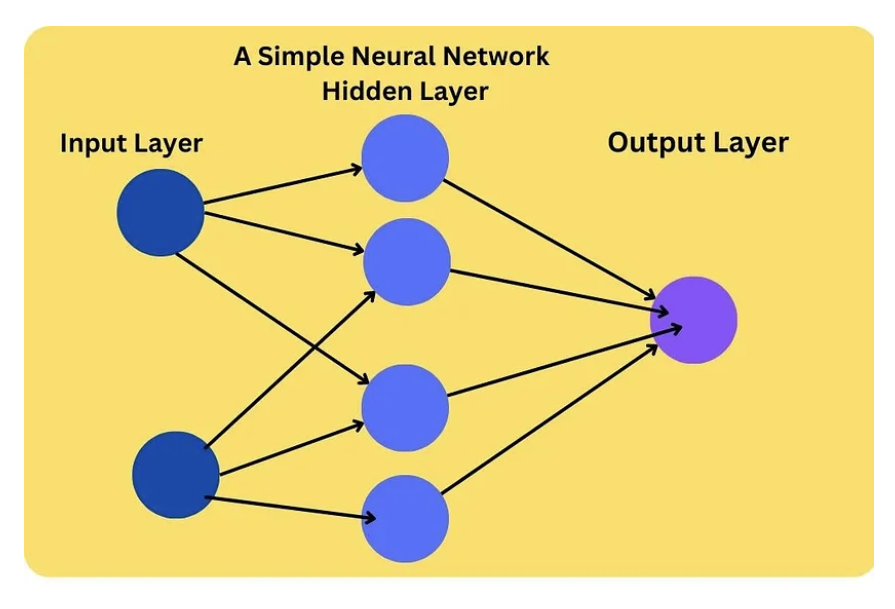
\includegraphics[scale=0.52]{./pics/ann.png}
  \caption[A simple Artificial Neural Network]{A simple Artificial Neural Network~\cite{ann}.}
  \label{fig:pi4}
\end{figure}

The most important concepts in an arbitrary ANN are:

\begin{itemize}
  \item \textbf{Input Data Layer}: This layer receives the raw information in many formats like images, strings or numbers.
  \item \textbf{Hidden Data Layers}: Located between output and input data layers, these layers are responsible for manipulating the received information through weighted connections and activation functions.
  \item \textbf{Output Data Layer}: The output data layer gives the answer of the query.
\end{itemize}

Training the neural network requires modifying the connection weights to reduce output errors. ANNs have proven effective across diverse applications such as Image and Speech Identification, Recommendation Systemsm, NLP, CV and more. Their capacity to train and evolve from data renders them invaluable in the fields of ML and AI.

\subsection{Multi-Layer Perceptron (MLP)}
Multilayer Perceptrons (MLPs) originated from the Perceptron, a SML algorithm created for problems with binary format classifications. The original Perceptron could only process very simple data distributions, which were linearly separable. To overcome this limitation, the Multilayer Perceptron was introduced, enabling the handling of both linearly separable and non-linearly separable data distributions~\cite{mlp}.

A Multilayer Perceptron is a type of NN which is a part of FFN class. In these neural architectures, the trainable parameters in one data layer are connected to the trainable parameters in the subsequent data layer in a forward manner, without any loops.

\begin{figure}[th]
  \centering
  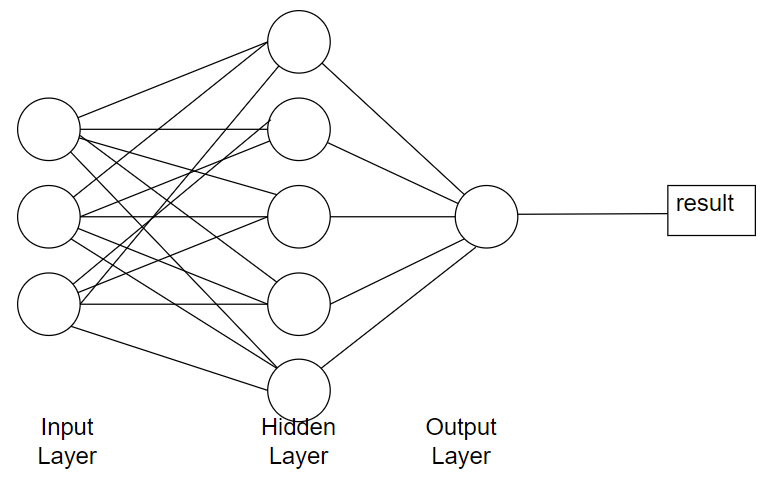
\includegraphics[scale=0.65]{./pics/mlp.png}
  \caption[Multilayer Perceptron]{Multilayer Perceptron~\cite{mlp}.}
  \label{fig:pi5}
\end{figure}

Moreover, MLP is a specific type of ANN distinguished by its layered architecture of interconnected neurons, intended to process data across multiple stages. The core components of an MLP include an input data layer, hidden data layers, an output data layer, functions with activations role, and a collection of neurons and train errors:

\begin{itemize}
  \item \textbf{Input Data Layer}: Receives various formats of information, like numbers, images or strings.
  \item \textbf{Hidden Data Layers}:
        Situated between the input and output layers, these intermediate layers are tasked with processing input data through intricate computations. There is typically no strict constraint on the number of hidden layers, although MLPs commonly include a moderate number to strike a balance between complexity and computational efficiency.
  \item \textbf{Output Data Layer}: The final layer serves as the ultimate stage where the network consolidates and presents the output results obtained from processing the data across its interconnected layers.
\end{itemize}


An essential characteristic of MLPs is their utilization of backpropagation, a SL method for neural networks learning. Backpropagation entails iteratively adjusting network neurons by propagating errors backward through the network starting from the output layer. This process enhances network performance by refining parameters and minimizing errors.

Due to their straightforward design, MLPs typically require shorter training periods to learn data representations and generate outputs. However, they often necessitate more powerful computing resources than standard computers, particularly devices equipped with Graphics Processing Units (GPUs), to handle the intensive computations involved.

MLPs have emerged as versatile and powerful tools across diverse domains, ranging from cutting-edge applications like Image Identification and NLP to the complex realm of computing in Financials. Their capacity to dynamically train from data and continually enhance performance underscores their pivotal role in advancing the frontiers of both Machine Learning and Artificial Intelligence.

\subsection{Generative Adversarial Network (GAN)}
Generative Adversarial Networks (GANs)~\cite{goodfellow2014generative} have revolutionized the field of Artificial Intelligence, capturing widespread attention for their ability to generate and enhance data in innovative ways. They are pivotal in a vast range of applications, like crafting photorealistic images, morphing artistic styles, and crafting realistic human faces with remarkable detail and fidelity. Introduced in a groundbreaking 2014 NeurIPS paper~\cite{goodfellow2014generative}, GANs are specialized Machine Learning systems designed to mimic specific data distributions~\cite{gan}.

At the heart of a GAN are two dynamically interacting models: a Generator, responsible for generating synthetic data, and a Discriminator, tasked with assessing the authenticity of the produced synthetic data. This dynamic interaction forms an adversarial training process, conceptualized as a competitive game. Of course, the network called Generator strives in generating very realistic information such that the network called Discriminator cannot reliably tell it apart from genuine data, achieving a 50\% deception rate.

A Generative Adversarial Network comprises two neural networks that engage in simultaneous adversarial training:

\begin{itemize}
  \item \textbf{Generator}: This network transforms random noise into coherent data outputs, such as images. Its objective is to generate data that closely resembles real-world data.
  \item \textbf{Discriminator}: This model evaluates both real and generated information from the Generator, attempting to differentiate between these. It produces a likelihood which tells if the provided information is real.
\end{itemize}

During training, the Generator iteratively enhances its capability to generate information that closely resembles real data, thereby challenging the Discriminator ability to distinguish between the two. Simultaneously, the Discriminator refines its proficiency in discerning genuine data from generated data. This competitive interplay drives the Generator to produce increasingly realistic data as training progresses, leading to a much better performance.

GANs utilize loss as a critical component of training the Generator and Discriminator, ensuring continuous improvement over time. The loss plays a pivotal role in adjusting the neurons of these NNs throughout the learning process to optimize their performance. In the context of GANs, both the generator and the discriminator commonly employ the binary cross-entropy loss. This loss quantifies the difference between the predicted outputs and the actual labels, facilitating effective learning and convergence of the network parameters towards generating more realistic data and improving discrimination accuracy:

\begin{equation}
  L = \frac{1}{N} \sum_{i=1}^{N} - (y_{i} \log(p_{i}) + (1 - y_{i}) \log(1 - p_{i}))
\end{equation}

In the above equation:
\begin{itemize}
  \item \( L \) is called the loss.
  \item \( y_{i} \) is called the true class label.
  \item \( p_{i} \) is the generated probability of the ith example which indicates its classification as belonging to class 1.
\end{itemize}

The Discriminator network goal is to accurately tell real examples as genuine and fake examples, created by the generator, as counterfeit. The function which is the loss for the discriminator is typically formulated as:

\begin{equation}
  -2L_D =  \mathbb{E}_{x \sim p_{data}(x)} [\log(D(x))] + \mathbb{E}_{z \sim p_z(z)} [\log(1 - D(G(z)))]
\end{equation}

where:

\begin{equation}
  \mathbb{E}_{x \sim p_{data}(x)} [f(x)] \approx \frac{1}{N} \sum_{i=1}^{N} f(x_i)
\end{equation}

\begin{equation}
  \mathbb{E}_{z \sim p_z(z)} [f(z)] \approx \frac{1}{M} \sum_{i=1}^{M} f(z_i)
\end{equation}

In these equations:
\begin{itemize}
  \item \( N \) is called the number of examples from the real distribution of information.
  \item \( M \) is called the number of examples from the fake distribution of information.
  \item \( x_i \) are examples from the real distribution of information.
  \item \( z_i \) are examples from the fake distribution of information.
\end{itemize}

This quantity $\mathbb{E}_{x \sim p_{data}(x)} [\log(D(x))]$ reprimands the network Discriminator for misidentifying genuine data, while this one $\mathbb{E}_{z \sim p_z(z)} [\log(1 - D(G(z)))]$ chastises it for incorrectly classifying the synthetic data produced by the network Generator.

In a Generative Adversarial Network (GAN), the Generator network objective is to fabricate samples that the Discriminator network cannot differentiate from authentic data. The Generator network loss function is meticulously crafted to impose penalties on the Generator whenever the Discriminator network successfully discerns its outputs as counterfeit. Mathematically, the Generator network loss function is articulated as follows:

\begin{equation}
  L_G = -\frac{1}{2} \mathbb{E}_{z \sim p_z(z)} \left[ \log(D(G(z))) \right]
\end{equation}

Here, \( z \) represents the noise input to the generator drawn from a prior distribution \( p_z(z) \), \( G(z) \) is the generated sample, and \( D(G(z)) \) is the discriminator probability that \( G(z) \) is a real sample.

The combined GAN loss, also known as the minimax loss, encapsulates the adversarial nature of GAN~\cite training. In this setup, the generator and discriminator engage in a two-player minimax game where the discriminator aims to maximize its ability to classify real and fake data correctly, while the generator strives to minimize the discriminator ability by generating realistic data. The combined loss is given by:

\begin{equation}
  L_{GAN} = \min_G \max_D (L_D + L_G)
\end{equation}

Here, \( L_D \) is the loss for the discriminator, and \( L_G \) is the loss for the generator.

Gradient penalty is a technique used to stabilize the training by penalizing the gradients if they become too steep. This can help in stabilizing the training and avoiding issues like mode collapse. The gradient penalty term is defined as:

\begin{equation}
  GP = \lambda \mathbb{E}_{\hat{x} \sim P_{\hat{x}}} \left[ \left( \| \nabla_{\hat{x}} D(\hat{x}) \|_2 - k \right)^2 \right]
\end{equation}

Where:
\begin{itemize}
  \item \(\mathbf{GP}\) represents the gradient penalty term.
  \item \(\mathbf{\lambda}\) is a hyperparameter that controls the strength of the penalty.
  \item The gradient component \(\nabla_{\hat{x}} D(\hat{x})\) is the gradient of the discriminator’s output with respect to its input \(\hat{x}\).
  \item \(\mathbf{P_{\hat{x}}}\) represents the distribution of interpolated samples between real and generated data.
  \item \(\mathbf{k}\) is a target norm for the gradient, often set to 1.
\end{itemize}

The purpose of introducing a gradient penalty is to enforce a constraint on the gradient of the discriminator output. This constraint ensures that the discriminator does not become overly confident, which can lead to sharp decision boundaries and unstable training. By keeping the gradient close to a target norm \(k\), typically set to 1, the gradient penalty helps maintain a smooth decision boundary.

The hyperparameter \(\lambda\) plays a crucial role in this process. A higher value of \(\lambda\) results in a stronger penalty for deviations from the target gradient norm, while a lower value of \(\lambda\) results in a weaker penalty. Proper tuning of \(\lambda\) is essential for the stability and performance of the GAN.

The interpolated samples \(\hat{x}\) are generated by taking convex combinations of real and generated samples. This interpolation helps in evaluating the gradient penalty across the data distribution, promoting better generalization and stability in the training process.

The discriminator loss with gradient penalty can be incorporated as follows:

\begin{equation}
  L_D = \mathbb{E}_{x \sim p_{\text{data}}(x)} \left[ \log(D(x)) \right] + \mathbb{E}_{z \sim p_z(z)} \left[ \log(1 - D(G(z))) \right] + GP
\end{equation}

This loss function consists of the usual GAN discriminator loss components for real and generated data, plus the gradient penalty term to regularize the discriminator behavior.


The discriminator loss with gradient penalty in GANs integrates standard loss components for real and generated data, augmented by a gradient penalty term to regulate the discriminator behavior. By penalizing large gradients, this method promotes smoother behavior in the discriminator, contributing to a more stable training process for both the generator and the discriminator. The gradient penalty helps prevent sharp changes in the discriminator output, which can otherwise lead to instability and issues like mode collapse, where the generator produces limited and repetitive outputs.

GANs are not only remarkable for their ability to create high-quality data, but also for their versatility across a range of complex tasks. Their unique adversarial training mechanism ensures that the generated data is continually refined, pushing the boundaries of what is possible in Machine Learning and Artificial Intelligence.

\begin{figure}[th]
  \centering
  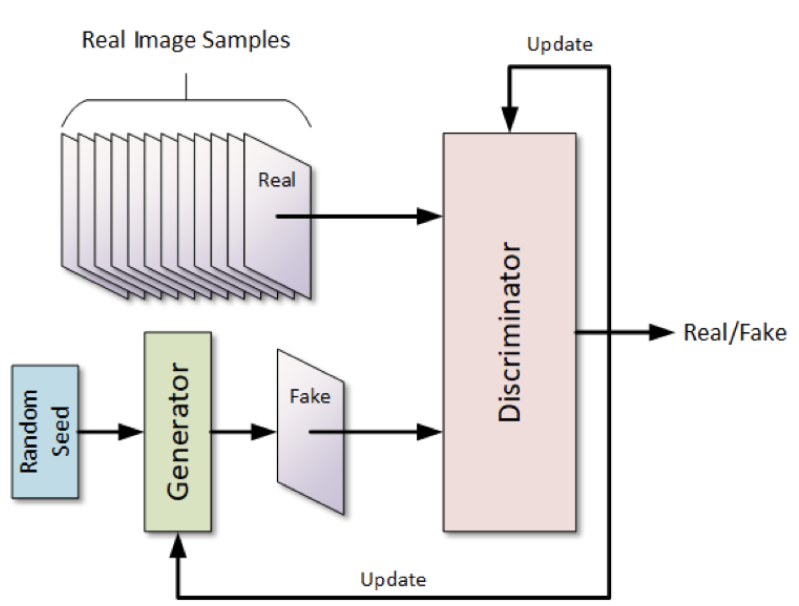
\includegraphics[scale=0.6]{./pics/gan.png}
  \caption[The Generative Adversarial Network Architecture]{The Generative Adversarial Network Architecture~\cite{gan-photo}.}
  \label{fig:pi6}
\end{figure}

\subsection{Visual Transformer (ViTs)}

Originally designed for Natural Language Processing, the Transformer~\cite{vaswani2017attention} architecture has been successfully adapted to other domains.

\begin{figure}[th]
  \centering
  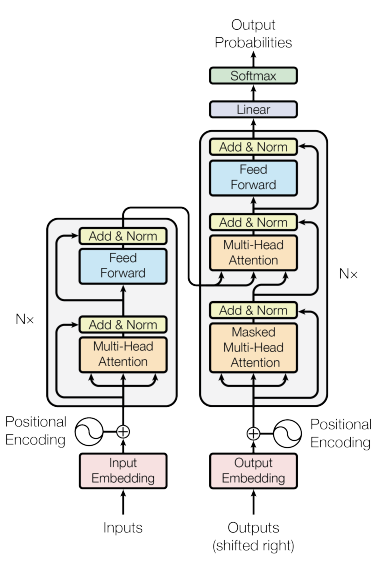
\includegraphics[scale=0.85]{./pics/transformer.png}
  \caption[The Transformer Architecture]{The Transformer Architecture~\cite{vaswani2017attention}.}
  \label{fig:pi7}
\end{figure}

An exemplary instance is the Vision Transformer (ViT)~\cite{dosovitskiy2020}, which tailors the Transformer architecture for Computer Vision applications. In ViTs, an image is segmented into a series of patches, each of which is linearly embedded and then treated as input tokens for a sequence of Transformer layers, collectively known as the Transformer Encoder.

The Vision Transformer (ViT) has attained SoTA performance on numerous image classification benchmarks, demonstrating the versatility and efficacy of the Transformer architecture across diverse domains.

Visual Transformer (ViT) is a Deep Learning architecture that leverages the self-attention mechanism of Transformers to process and understand visual data such as images.

By dividing an input image into smaller patches, ViT allows each patch to attend to others, leading to state-of-the-art performance in various computer vision tasks

The usual workflow of Visual Transformers in Image Classification task include~\cite{vit}:

\begin{enumerate}
  \item Decomposing the Image into Patches
        \begin{itemize}
          \item \textbf{Input Image}: Consider an input image with dimensions \( H \times W \times N \), where \( H \) is the height, \( W \) is the width, and \( N \) represents the number of channels (such as 3 for RGB images).
          \item \textbf{Patch Flattening}: The image is divided into smaller patches, each of size \( 16 \times 16 \) pixels. For an RGB image, this results in each patch being flattened into a vector of 768 elements (since \( 16 \times 16 \times 3 = 768 \)). This transformation converts the spatial information of the image patches into a form suitable for further processing by the Vision Transformer.
        \end{itemize}

  \item Patch Embedding
        \begin{itemize}
          \item \textbf{Linear Transformation}: Each flattened patch undergoes a trainable linear transformation that maps it into a \( D \)-dimensional embedding space. This operation, which is akin to a fully connected layer, enriches the representation of each patch, making it more suitable for subsequent processing by the transformer.
          \item \textbf{Spatial Information Encoding}: Since the transformer architecture does not inherently preserve the spatial arrangement of patches, additional spatial information is incorporated into the patch embeddings. This is achieved by adding positional encodings, which can be either fixed or learned parameters, to the embedded patches. These encodings ensure that the model retains information about the position of each patch within the original image.
        \end{itemize}

  \item Visual Transformer Encoder
        \begin{itemize}
          \item \textbf{Self-Attention Mechanism}: At the heart of the transformer model lies the self-attention mechanism, which efficiently evaluates the relevance of different patches in relation to each other for a specific task. This mechanism determines the amount of focus each part of the image should receive when encoding a particular patch, enhancing the model ability to understand complex relationships within the image.
          \item \textbf{Multi-head Attention}: The encoder employs multi-head attention, running several self-attention mechanisms in parallel. This approach allows the model to simultaneously capture diverse aspects and patterns in the image, enriching the representation of each patch with a variety of contextual information.
          \item \textbf{Feed-forward Network}: Following the attention computation, each patch representation is processed through a feed-forward neural network (FFNN). This network is applied identically and independently to each position, further refining the encoded information and enabling the model to learn intricate features.
          \item \textbf{Residual Connections and Normalization}: To ensure a stable training process and facilitate the accumulation of knowledge from each layer, the transformer encoder incorporates residual connections around each sub-layer. These are followed by layer normalization, which helps maintain consistent gradients and improves the overall training dynamics, ensuring that each layer effectively builds upon the previous ones.
        \end{itemize}

  \item Creating the Output
        \begin{itemize}
          \item \textbf{CLS Token}: To adapt transformer architecture for image classification, a dedicated classification token (CLS) is prefixed to the sequence of embedded patches. This token encapsulates comprehensive information aggregated from the entire image after undergoing transformation through the encoder. Utilized by a classifier, typically a straightforward linear layer, it facilitates accurate prediction of the image class by leveraging enriched contextual understanding encoded within the transformer model.
        \end{itemize}

  \item Training
        \begin{itemize}
          \item \textbf{Optimizing Model Parameters}: During training, the transformer model is fine-tuned end-to-end using an appropriate loss function, commonly cross-entropy for classification tasks. This function calculates the discrepancy between predicted and actual class labels, guiding the optimization of parameters across the linear projection, transformer encoder, and classifier. The objective is to systematically minimize this loss on a training dataset, ensuring the model effectively learns to classify images with high accuracy.
        \end{itemize}
\end{enumerate}

\begin{figure}[th]
  \centering
  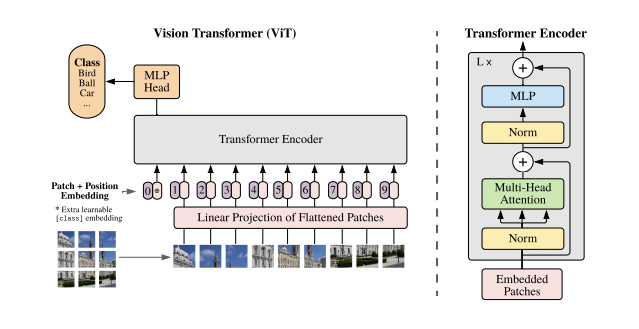
\includegraphics[scale=0.8]{./pics/vit.png}
  \caption[The Visual Transformer Neural Architecture]{The Visual Transformer Neural Architecture~\cite{vaswani2017attention, dosovitskiy2020}.}
  \label{fig:p8}
\end{figure}

The transformation at each layer can be defined as~\cite{Comajoan_Cara_2024}:

\begin{equation}
  W = X + \text{MHA}(\text{Norm}(X), \text{Norm}(X), \text{Norm}(X))
\end{equation}

\begin{equation}
  X' = W + \text{MLP}(\text{Norm}(W))
\end{equation}

where \( X \in \mathbb{R}^{N \times D} \) is a Transformer layer matrix input and  \( X' \in \mathbb{R}^{N \times D} \) is the output.

The attention mechanism is a crucial element of the Transformer architecture, allowing the model to concentrate on particular segments of the input sequence while generating each output component. Given a query matrix \( Q \in \mathbb{R}^{N \times D_k} \), a key matrix \( K \in \mathbb{R}^{M \times D_k} \), and a value matrix \( V \in \mathbb{R}^{M \times D_v} \), the attention is defined as~\cite{Comajoan_Cara_2024}:

\begin{equation}
  \text{Attention}(V, K, Q) = \text{softmax}\left(\frac{QK^T}{\sqrt{D_k}}\right) V
\end{equation}

where \( D_k \) is the dimension of the keys, used as a scaling factor to prevent the dot products from becoming excessively large.

Self-attention is a distinct type of attention in which the query, key, and value matrices are all derived from the same input matrix \( X \).  In the Transformer architecture, self-attention allows each position in the input sequence to consider all other positions in the preceding layer.


Multi-head attention enhances the attention mechanism, allowing the model to simultaneously focus on information from various representation subspaces at different positions. Instead of performing a single attention operation, multi-head attention sends the queries, keys, and values \( h \) times using different trained linear projections. These projections are processed in parallel, their results concatenated, and the concatenated output is then linearly projected once more. Mathematically, multi-head attention is expressed as~\cite{Comajoan_Cara_2024}:

\begin{equation}
  \text{MHA}(V, K, Q) = \text{Concat}(\text{single\_head}_i) W^O, i=1:h
\end{equation}

\begin{equation}
  \text{single\_head}_i = \text{Attention}(V W_i^V, K W_i^K, Q W_i^Q)
\end{equation}

Here, \( W_i^K \in \mathbb{R}^{D_x \times D_k} \), \( W_i^V \in \mathbb{R}^{D_x \times D_v} \), \( W_i^Q \in \mathbb{R}^{D_x \times D_k} \), and \( W^O \in \mathbb{R}^{h D_v \times D_x} \) are trainable neurons.


\subsection{Learning Rate Schedulers}
When training deep networks, it is beneficial to gradually reduce the learning rate as the training progresses. This concept stems from the idea that a high learning rate imparts high kinetic energy to the model, causing its parameter vector to oscillate chaotically. Consequently, the model struggles to stabilize within the deeper and narrower valleys of the loss function, which represent local minima. Conversely, if the learning rate is too low, the system exhibits low kinetic energy, leading it to settle into the shallower and narrower valleys of the loss function, often getting stuck in suboptimal minima.

In essence, starting with a higher learning rate helps the model explore the loss landscape broadly, avoiding premature convergence. As training advances, lowering the learning rate allows the model to fine-tune its parameters and settle into more optimal solutions, thus achieving better performance. This dynamic adjustment helps in navigating the complex loss surfaces typical in deep learning, striking a balance between exploration and exploitation~\cite{learningrate}.

Examples of Learning Rate Scheduling~\cite{learningrate2}:

\begin{itemize}
  \item \textbf{ExponentialLR}: Adjusts the learning rate by dividing it by a factor each epoch or evaluation period.
  \item \textbf{CyclicLR}: Oscillates the learning rate cyclically between specified minimum and maximum values.
  \item \textbf{StepLR}: Decreases the learning rate by multiplying it with a decay factor every fixed number of epochs or evaluation periods.
  \item \textbf{MultiStepLR}: Reduces the learning rate by a factor when the training reaches predefined milestones.
  \item \textbf{ReduceLROnPlateau}: Dynamically reduces the learning rate if a monitored metric fails to improve for a certain number of evaluations.
  \item \textbf{CosineAnnealingLR}: Starts with a high learning rate and smoothly decreases it following a cosine curve, periodically restarting the cycle.
\end{itemize}

\subsection{Weight Decay}
Weight decay, also known as L2 regularization, is an essential technique in deep learning to enhance model performance. By penalizing large weights, it offers several key benefits~\cite{weightdecay}:

\begin{itemize}
  \item \textbf{Mitigates Overfitting:} Large weights often cause a model to memorize training data, hindering its ability to generalize to new examples. Weight decay discourages large weights, promoting the learning of smaller, more generalizable weights that capture the fundamental patterns in the data.

  \item \textbf{Enhances Model Stability:} Large weights can destabilize training and increase sensitivity to data noise. Weight decay stabilizes the training process by keeping weights manageable, thus enhancing the model robustness and reducing overfitting.

  \item \textbf{Encourages Feature Sharing:} By promoting similar weights across different neurons, weight decay fosters feature sharing. This leads to a more efficient network where multiple neurons can utilize the same features, often resulting in fewer required parameters.

  \item \textbf{Boosts Generalization in Overparameterized Models:} Modern deep learning models often contain more parameters than training data, a scenario known as overparameterization. Weight decay helps manage the complexity of such models, improving their ability to generalize.
\end{itemize}

Weight decay adds a penalty to the loss function, proportional to the sum of the squared weights. This penalty encourages the model to prefer smaller weights during training. Implementation of weight decay typically follows one of two approaches:

\begin{itemize}
  \item \textbf{L2 Regularization:} Adds a term to the loss function proportional to the sum of the squared weights.
  \item \textbf{Optimizer-based Weight Decay:} Alters the optimizer update rule to include a decay factor that incrementally reduces the weights.
\end{itemize}

Choosing the right weight decay parameter involves balancing overfitting prevention with performance optimization. The optimal value varies based on model size, complexity, training data, and learning rate. Techniques such as grid search, hyperparameter optimization, and cross-validation are useful for identifying the best weight decay value.

\subsection{Cross Validation}
Cross-Validation (CV) is a cornerstone of evaluating learning models which provides the possibility to approximate model performance on unseen data not used while training. When training a model, the dataset is divided into two primary subsets: training and testing. The training set encompasses all the examples from which the model learns, while the testing set emulates real-world scenarios where the model performance is assessed~\cite{crossvalidation}.

Validating a learning model before deploying it in production involves ensuring it can make accurate predictions on data it has never encountered. This unseen data represents any type of information that the model hasn't been trained on. Ideally, during testing, this data flows directly into the model across numerous iterations. However, in practice, access to genuinely new data is often restricted or unavailable in a fresh environment.

A common approach is the 80-20 rule, where 80\% of the data is used for training and 20\% for testing. Despite its popularity, this method is prone to creating a seemingly perfect split that might artificially inflate model accuracy, while failing to replicate the same performance in real-world scenarios. The accuracy achieved in such cases can often be attributed to mere chance. It is worth noting that the 80-20 split is not a hard and fast rule; other ratios like 70-30 or 75-25 are frequently used as well.

Tuning model hyperparameters is another crucial step in optimizing an algorithm to uncover the hidden patterns within a dataset. However, performing this tuning on a simple training-testing split is generally discouraged. Model performance is highly sensitive to hyperparameters, and adjusting them based on a fixed data split can lead to overfitting, reducing the model generalizability.

To avoid overfitting during hyperparameter tuning, some suggest dividing the dataset into three parts: training, validation, and testing, for example, using 70\% for training, 20\% for validation, and 10\% for testing. Yet, with small datasets, maximizing the data for training is often necessary. Moreover, such splits can introduce bias if important examples are disproportionately allocated to the training or validation sets. Cross-validation (CV) is a valuable technique to mitigate these issues by ensuring a more balanced evaluation.

The process of splitting data for training and testing can be fraught with difficulties. The testing set may not share similar properties with the training set, causing instability. Even though random sampling theoretically gives each sample an equal chance of being included in the testing set, a single split might still result in instability when the experiment is repeated.


\subsection{Random Search}
Random Search is a hyperparameter optimization technique in machine learning that samples a defined number of hyperparameter combinations from specified distributions at random. These distributions represent sets or ranges of possible parameter values~\cite{randomsearch}.

This method efficiently navigates a subset of the hyperparameter space, making it faster and more resource-efficient compared to exhaustive techniques like grid search.

Although Random Search may not guarantee the discovery of the absolute optimal hyperparameters, it is highly effective at identifying good configurations, particularly in scenarios involving large or complex parameter spaces.

The Random Search process begins by initializing random hyperparameter values from the defined search space, denoted as point \(x\). The value of the cost function is then evaluated at \(x\). Subsequently, another set of random hyperparameter values, labeled \(y\), is generated, and the cost function is computed at this new point \(y\).

If the cost function value at \(y\) is lower than that at \(x\), the algorithm updates the starting point to \(y\) by setting \(x = y\). This iterative process continues: generating new random points, comparing cost function values, and updating the starting point if a better set of hyperparameters is found. The procedure repeats until a stopping criterion specified by the user is met~\cite{randomsearch2}.

Some advantages of random search in Machine Learning over grid search are:

\begin{itemize}
  \item Random search tends to yield better results than grid search, especially when the dimensionality and the number of hyperparameters are high.
  \item Random search allows for limiting the number of hyperparameter combinations, whereas grid search exhaustively evaluates all possible combinations.
  \item Typically, random search achieves superior results compared to grid search in fewer iterations.
\end{itemize}

\section{Ordinary Differential Equations (ODE)}
Differential equations are pivotal in capturing and describing the dynamics of various physical, biological, and engineering systems. Among these, Ordinary Differential Equations (ODEs) hold a special place. ODEs are equations involving functions of a single independent variable and their derivatives. They are termed ordinary to distinguish them from partial differential equations, which involve multiple independent variables.

An ODE is formulated as an equation involving an unknown function \( f(x) \), its derivatives, and the independent variable \( x \). It is being assumed that \( f(x) \) is differentiable up to order \( k \). The general form of an ODE of order \( k \) is expressed as~\cite{odes}:

\begin{equation}
  G\left(x, f(x), \frac{df}{dx}, \ldots, \frac{d^k f}{dx^k}\right) = 0,
\end{equation}

where the function \( G \) includes the highest derivative \( \frac{d^k f}{dx^k} \). The order of the ODE is determined by the highest derivative present. The degree of the ODE is the power of the highest derivative after clearing any fractional powers.

An ODE is called linear if \( G \) is a linear function of \( f(x) \) and its derivatives:

\begin{equation}
  a_k(x) \frac{d^k f}{dx^k} + a_{k-1}(x) \frac{d^{k-1} f}{dx^{k-1}} + \cdots + a_1(x) \frac{df}{dx} + a_0(x) f = h(x).
\end{equation}

Otherwise, it is nonlinear.

The general form provided is often referred to as the implicit form. In an explicit form, the highest-order derivative is expressed as a function of lower-order derivatives:

\begin{equation}
  \frac{d^k f}{dx^k} = F\left(x, f(x), \frac{df}{dx}, \ldots, \frac{d^{k-1} f}{dx^{k-1}}\right).
\end{equation}

To uniquely determine a solution to an ODE, initial conditions are necessary. These conditions specify the value of the function and its derivatives at a particular point. For a first-order ODE, an initial condition might look like:

\begin{equation}
  f(x_0) = f_0,
\end{equation}

where \( x_0 \) is the initial point, and \( f_0 \) is the value of the function at \( x_0 \).

For a second-order ODE, two initial conditions are typically required:

\begin{equation}
  f(x_0) = f_0 \quad \text{and} \quad \frac{df}{dx}\Big|_{x=x_0} = f_1.
\end{equation}

Let us consider a specific example of an ODE for the function \( f(x) \):

\begin{equation}
  \frac{d^2 f}{dx^2} = 5 \left[1 + \left(\frac{df}{dx}\right)^{\frac{2}{3}}\right]^{\frac{1}{3}}.
\end{equation}

This equation is a nonlinear explicit ODE of degree 3 and order 2. The nonlinearity arises from the fractional power of the first derivative term.

Solving an ODE involves finding the function \( f(x) \) that satisfies the equation over the domain of \( x \) (e.g., \( \mathbb{R} \)). Various methods can be employed depending on the nature of the ODE, including analytical techniques, such as separation of variables, integrating factors, and numerical approaches, such as Euler's method, Runge-Kutta methods.

ODEs are essential tools in modeling and understanding the behavior of dynamic systems. Their solutions provide insight into how systems evolve over time under various conditions.

\section{Runge-Kutta Methods}
Runge-Kutta methods are a family of iterative methods used to solve initial value problems for ordinary differential equations (ODEs). These methods vary in their order of accuracy, with higher-order methods providing more accurate solutions. Here,the formulations for the 1st, 2nd, 3rd, and 4th order Runge-Kutta methods are being presented~\cite{odes}.

The simplest Runge-Kutta method is the 1st order method, also known as Euler's Method. It is given by:

\begin{equation}
  y_{i+1} = y_i + h f(y_i, x_i).
\end{equation}

This method has a local truncation error of \( O(h^2) \) and a global truncation error of \( O(h) \).

The 2nd order Runge-Kutta method improves upon Euler's method by incorporating an additional intermediate step. One common form is the Heun's method, given by:

\begin{equation}
  k_{1i} = f(y_i, x_i),
\end{equation}

\begin{equation}
  k_{2i} = f(y_i + h k_{1i}, x_i + h),
\end{equation}

\begin{equation}
  y_{i+1} = y_i + \frac{h}{2} (k_{1i} + k_{2i}).
\end{equation}

Another popular 2nd order method is the midpoint method:

\begin{equation}
  k_{1i} = f(y_i, x_i),
\end{equation}

\begin{equation}
  k_{2i} = f(y_i + \frac{h}{2} k_{1i}, x_i + \frac{h}{2}),
\end{equation}

\begin{equation}
  y_{i+1} = y_i + h k_{2i}.
\end{equation}

Both methods have a local truncation error of \( O(h^3) \) and a global truncation error of \( O(h^2) \).

The 3rd order Runge-Kutta method provides even greater accuracy. It is formulated as follows:

\begin{equation}
  k_{1i} = f(y_i, x_i),
\end{equation}

\begin{equation}
  k_{2i} = f\left(y_i + \frac{h}{2} k_{1i}, x_i + \frac{h}{2}\right),
\end{equation}

\begin{equation}
  k_{3i} = f\left(y_i - h k_{1i} + 2h k_{2i}, x_i + h\right),
\end{equation}

\begin{equation}
  y_{i+1} = y_i + \frac{h}{6} (k_{1i} + 4k_{2i} + k_{3i}).
\end{equation}

This method has a local truncation error of \( O(h^4) \) and a global truncation error of \( O(h^3) \).

The 4th order Runge-Kutta method is the most widely used due to its high accuracy and relatively simple implementation. It is given by:

\begin{equation}
  k_{1i} = f(y_i, x_i),
\end{equation}

\begin{equation}
  k_{2i} = f\left(y_i + \frac{h}{2} k_{1i}, x_i + \frac{h}{2}\right),
\end{equation}

\begin{equation}
  k_{3i} = f\left(y_i + \frac{h}{2} k_{2i}, x_i + \frac{h}{2}\right),
\end{equation}

\begin{equation}
  k_{4i} = f(y_i + h k_{3i}, x_i + h),
\end{equation}

\begin{equation}
  y_{i+1} = y_i + \frac{h}{6} (k_{1i} + 2k_{2i} + 2k_{3i} + k_{4i}).
\end{equation}

This method has a local truncation error of \( O(h^5) \) and a global truncation error of \( O(h^4) \).

The Runge-Kutta methods of various orders offer a range of options for solving initial value problems in ODEs, with higher-order methods providing greater accuracy. The choice of method depends on the desired balance between computational complexity and accuracy.

\subsection{ODE Interpretation of Transformer Layers}
Residual networks can be viewed as an Euler discretization of the solutions to Ordinary Differential Equations (ODEs). Building on this concept, delving deeper into the relationship between Transformers and numerical ODE methods it can be demonstrated that a residual block of layers within a Transformer can be interpreted as a higher-order solution to an ODE~\cite{li2022ode}.

Let \( Y^m = [y_1^m, y_2^m, \ldots, y_L^m] \) represent the input to the \( m \)-th transformer layer, where \( L \) denotes the sequence length. The multi-head attention sublayer can be mathematically expressed as~\cite{zhong2022neural}:

\begin{equation}\label{eq:1}
  \hat{y}_i^m = y_i^m + G(y_i^m, Y^m), \quad 1 \leq i \leq L,
\end{equation}

where \( G \) represents the multi-head dot-product attention function.

The output from this sublayer, denoted by \( \hat{Y}^m = [\hat{y}_1^m, \hat{y}_2^m, \ldots, \hat{y}_L^m] \), is then fed into the feedforward network sublayer. The transformation in this sublayer is given by:

\begin{equation}\label{eq:2}
  y_i^{m+1} = \hat{y}_i^m + H(\hat{y}_i^m), \quad 1 \leq i \leq L,
\end{equation}

where \( H \) represents the sequence of linear mappings and activation functions.

The operations in equations \ref{eq:1} and \ref{eq:2} can be viewed as a numerical integration scheme over the time interval \([m, m+1]\) of the following ODE, using the Lie-Trotter decomposing method ~\cite{lu2019understanding, dutta2021redesigning}:
\begin{equation}
  \frac{dy_i}{dt} = H(y_i) + G(y_i, Y).
\end{equation}

Where \( Y = [{y}_1, {y}_2, \ldots, {y}_L] \). This interpretation provides a deeper understanding of the Transformer internal mechanisms by linking them to the well-established principles of numerical integration.

Writing $H(y_i)$ and $G(y_i, Y)$ in terms of a new function, namely $F(y_i, Y) = H(y_i) + G(y_i, Y)$, and keeping in mind that the function $F(y_i, Y)$ is re-used in a block and the input $Y$ is shared within the block, Runge-Kutta blocks can be computed as follows:

\begin{equation}
  y_i(t + 1) = y_i(t) + \sum_{j=1}^{n}\gamma_{j}F_{ij}
\end{equation}
\begin{equation}
  F(y_i, Y) = F_i
\end{equation}
\begin{equation}
  F_{ij} = F_i(y_i + \sum_{p=1}^{j-1}\beta_{jp}F_{ip}, Y)
\end{equation}

Where $\beta$ is a coefficient which can be determined by the Taylor series of $y_i(t+1)$ This makes the neural network more parameter-efficient~\cite{li2022ode}.

Thus, the definiton of Euler's method is (RK1):

\begin{equation}
  y_i(t + 1) = y_i(t) + F_{i1}
\end{equation}
\begin{equation}
  F_{i1} = F_i(y_i(t), Y)
\end{equation}

One can define a second order Runge-Kutta block as (RK2):

\begin{equation}
  y_i(t + 1) = y_i(t) + \frac{1}{2}(F_{i1} + F_{i2})
\end{equation}
\begin{equation}
  F_{i1} = F_i(y_i(t), Y)
\end{equation}
\begin{equation}
  F_{i2} = F_i(y_i(t) + F_{i1}, Y) = F_i(y_i(t) + F_i(y_i(t), Y), Y)
\end{equation}

And a third order Runge-Kutta block as (RK3):

\begin{equation}
  y_i(t + 1) = y_i(t) + \frac{1}{9}(2F_{i1} + 3F_{i2} + 4F_{i3})
\end{equation}
\begin{equation}
  F_{i1} = F_i(y_i(t), Y)
\end{equation}
\begin{equation}
  F_{i2} = F_i(y_i(t) + \frac{1}{2}F_{i1}, Y) = F_i(y_i(t) + \frac{1}{2}F_i(y_i(t), Y), Y)
\end{equation}
\begin{equation}
  F_{i3} = F_i(y_i(t) + \frac{3}{4}F_{i2}, Y) = F_i(y_i(t) + \frac{3}{4}F_i(y_i(t) + \frac{1}{2}F_i(y_i(t), Y), Y), Y)
\end{equation}

Likewise, a fourth order Runge-Kutta block can be written as (RK4):

\begin{equation}
  y_i(t + 1) = y_i(t) + \frac{1}{6}(F_{i1} + 2F_{i2} + 2F_{i3} + F_{i4})
\end{equation}
\begin{equation}
  F_{i1} = F_i(y_i(t), Y)
\end{equation}
\begin{equation}
  F_{i2} = F_i(y_i(t) + \frac{1}{2}F_{i1}, Y) = F_i(y_i(t) + \frac{1}{2}F_i(y_i(t), Y), Y)
\end{equation}
\begin{equation}
  F_{i3} = F_i(y_i(t) + \frac{1}{2}F_{i2}, Y) = F_i(y_i(t) + \frac{1}{2}F_i(y_i(t) + \frac{1}{2}F_i(y_i(t), Y), Y), Y)
\end{equation}
\begin{equation}
  F_{i4} = F_i(y_i(t) + F_{i3}, Y) = F_i(y_i(t) + F_i(y_i(t) + \frac{1}{2}F_i(y_i(t) + \frac{1}{2}F_i(y_i(t), Y), Y), Y), Y)
\end{equation}

\begin{figure}[th]
  \centering
  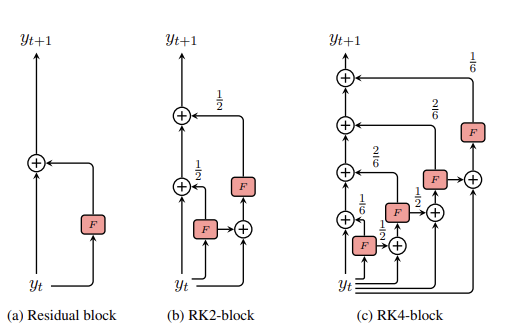
\includegraphics[scale=1]{./pics/odes.png}
  \caption[Different Runge-Kutta ODEs Blocks]{Different Runge-Kutta ODEs Blocks~\cite{li2022ode}.}
  \label{fig:p9}
\end{figure}

However, further optimizations can still be made for deeper models in terms of minimizing the vanishing gradient effects. Considering RK4:
\begin{equation}
  y_i(t + 1) = y_i(t) + \frac{1}{6}(F_{i1} + 2F_{i2} + 2F_{i3} + F_{i4})\label{eq:3}
\end{equation}

Let $\mathcal{E}$ be the loss of training, $L$ be the number blocks of the model, and $y_{iL}$ be the model output. The gradient of $\mathcal{E}$ at $y_{it}$, using the Chain Rule, is:

\begin{equation}
  \frac{\partial \mathcal{E}}{\partial y_{it}} = \frac{\partial \mathcal{E}}{\partial y_{iL}} \cdot \frac{\partial y_{iL}}{\partial y_{iL-1}} \cdot \frac{\partial y_{iL-1}}{\partial y_{iL-2}} \dots \frac{\partial y_{it+1}}{\partial y_{it}}
\end{equation}
\begin{equation}\label{eq:4}
  \frac{\partial \mathcal{E}}{\partial y_{it}} = \frac{\partial \mathcal{E}}{\partial y_{iL}} \cdot \prod_{k=t}^{L-1} \frac{\partial y_{ik+1}}{\partial y_{ik}}
\end{equation}

where
\begin{align}\label{eq:5}
  \frac{\partial y_{ik+1}}{\partial y_{ik}} = & \ 1 + \frac{1}{6}\frac{\partial F_i(y_{ik}, Y)}{\partial y_{ik}} \notag  +                                                                                                                                                                         \\
                                              & \frac{1}{3}\frac{\partial F_i(y_{ik} + \frac{1}{2}F_i(y_{ik}, Y), Y)}{\partial y_{ik} + \frac{1}{2}F_i(y_{ik}, Y)} \cdot \left( 1 + \frac{1}{2}\frac{\partial F_i(y_{ik}, Y)}{\partial y_{ik}} \right) \notag +                                    \\
                                              & \frac{1}{3}\frac{\partial F_i(y_{ik} + \frac{1}{2}F_i(y_{ik} + \frac{1}{2}F_i(y_{ik}, Y), Y), Y)}{\partial y_{ik} + \frac{1}{2}F_i(y_{ik} + \frac{1}{2}F_i(y_{ik}, Y), Y)} \cdot \notag                                                            \\
                                              & \ \ \ \ \left[ 1 + \frac{1}{2}\frac{\partial F_i(y_{ik} + \frac{1}{2}F_i(y_{ik}, Y), Y)}{\partial y_{ik} + \frac{1}{2}F_i(y_{ik}, Y)} \cdot \left( 1 + \frac{1}{2}\frac{\partial F_i(y_{ik}, Y)}{\partial y_{ik}} \right)\right] \notag +          \\
                                              & \frac{1}{6}\frac{\partial F_i(y_{ik} + F_i(y_{ik} + \frac{1}{2}F_i(y_{ik} + \frac{1}{2}F_i(y_{ik}, Y), Y), Y), Y)}{\partial y_{ik} + F_i(y_{ik} + \frac{1}{2}F_i(y_{ik} + \frac{1}{2}F_i(y_{ik}, Y), Y), Y)} \cdot \notag                          \\
                                              & \ \ \ \ \left\{ 1 + \frac{\partial F_i(y_{ik} + \frac{1}{2}F_i(y_{ik} + \frac{1}{2}F_i(y_{ik}, Y), Y), Y)}{\partial y_{ik} + \frac{1}{2}F_i(y_{ik} + \frac{1}{2}F_i(y_{ik}, Y), Y)} \cdot \right. \notag                                           \\
                                              & \ \ \ \ \left. \left[ 1 + \frac{1}{2} \frac{\partial F_i(y_{ik} + \frac{1}{2}F_i(y_{ik}, Y), Y)}{\partial y_{ik} + \frac{1}{2}F_i(y_{ik}, Y)} \cdot \left( 1 + \frac{1}{2}\frac{\partial F_i(y_{ik}, Y)}{\partial y_{ik}} \right) \right] \right\}
\end{align}

This result can lead to a big problem of gradient vanishing when $L$ is big.

The issue seems to stem from the small coefficients of $F_i$, specifically, $\gamma_1 = \gamma_4 = \frac{1}{6}$ and $\gamma_2 = \gamma_3 = \frac{1}{3}$. A practical approach is to empirically set $\gamma_i = 1$, $\beta_p = 1$ for removing the product factors that are less than 1 during gradient computation. Furthermore, experiments shown that eliminating $F_{i2}$ and $F_{i3}$ blocks can lead to a faster convergence and a small accuracy increase.

However, this adjustment is not theoretically supported by traditional Runge-Kutta methods. Eq. \ref{eq:3} with the updated coefficients can be written as:

\begin{equation}
  y_i(t + 1) = y_i(t) + F_{i1} + F_{i4}
\end{equation}

Then, with all of the transformations, the gradient of loss will become:

\begin{equation}
  \frac{\partial \mathcal{E}}{\partial y_{it}} = \frac{\partial \mathcal{E}}{\partial y_{iL}} \cdot \prod_{k=t}^{L-1} f_{ik}
\end{equation}

where
\begin{align}
  f_{ik} = & \ 1 + \frac{\partial F_i(y_{ik}, Y)}{\partial y_{ik}} + \frac{\partial F_i(y_{ik} + F_i(y_{ik} + F_i(y_{ik} + F_i(y_{ik}, Y), Y), Y), Y)}{\partial y_{ik} + F_i(y_{ik} + F_i(y_{ik} + F_i(y_{ik}, Y), Y), Y)} \cdot \notag \\
           & \ \ \ \ \left\{ 1 + \frac{\partial F_i(y_{ik} + F_i(y_{ik} + F_i(y_{ik}, Y), Y), Y)}{\partial y_{ik} + F_i(y_{ik} + F_i(y_{ik}, Y), Y)} \cdot \right. \notag                                                               \\
           & \ \ \ \ \left. \left[ 1 + \frac{\partial F_i(y_{ik} + F_i(y_{ik}, Y), Y)}{\partial y_{ik} + F_i(y_{ik}, Y)} \cdot \left( 1 + \frac{\partial F_i(y_{ik}, Y)}{\partial y_{ik}} \right) \right] \right\}
\end{align}
\\
Understanding the transformer layer operations through the lens of numerical integration opens up new avenues for improving their efficiency and effectiveness by leveraging advanced techniques from numerical analysis.

\section{Quantum Computing}
Quantum computing revolutionizes information processing by utilizing qubits instead of classical bits. Unlike classical bits, qubits can exist in multiple states at once due to superposition. The state of \(n\) qubits is represented by a unit vector \(\left| \psi \right\rangle\) in the Hilbert space \(\mathbb{C}^{2^n}\). In this context, the ket \(\left| \cdot \right\rangle\) represents a column vector, while the bra \(\left\langle \cdot \right|\) represents a row vector.

An \(n\)-level quantum system is described by an \(n\)-dimensional Hilbert space \(\mathcal{H}^n\). A quantum pure state is represented by a unit complex vector \(\mathbf{v}\) in \(\mathcal{H}^n\). This state can be depicted as a density matrix \(\rho = \mathbf{v} \mathbf{v}^\dagger\), where \(\mathbf{v}^\dagger\) is the conjugate transpose of \(\mathbf{v}\). For a mixture of pure states \(\{ \mathbf{v}_i \}_{i=1}^n\) with probabilities \(\{ p_i \}_{i=1}^n\) summing to 1, the mixed state density matrix is \(\rho = \sum_{i=1}^n p_i \mathbf{v}_i \mathbf{v}_i^\dagger\).~\cite{fan2024Quantum}.

The evolution of a closed quantum system is governed by unitary transformations~\cite{nielsen2001quantum}. The state \(\mathbf{v}_t\) at time \(t\) evolves to \(\mathbf{v}_{t+\Delta t}\) at time \(t + \Delta t\) via a unitary matrix \(U \in \mathcal{H}\), such that \(U_{\Delta t} \mathbf{v}_t = \mathbf{v}_{t+\Delta t}\). This matrix \(U\) satisfies \(UU^\dagger = I\). Considering a density matrix \(\rho\), the system evolution is expressed as \(U \rho_t U^\dagger = \rho_{t+\Delta t}\).

A quantum circuit manipulates qubits through a series of quantum gates, transforming their states via unitary operations. Mathematically, this is represented as \(U \left| \psi \right\rangle\), where \(U\) is a \(2^n \times 2^n\) unitary matrix. The circuit typically concludes with the measurement of qubits, revealing the final state of the system.

In this context, $R_X$, $R_Y$ and $R_Z$ gates are used, which rotates a qubit around the $X$, $Y$ and $Z$ axes, and CNOT gates, which flips the state of a target qubit conditionally on the state of a control qubit being \(\left| 1 \right\rangle\). The Hadamard gate $H$ helps with the creation of entanglement, along with CNOT.

These gates are defined by the following matrices:

\[
  H = \frac{1}{\sqrt{2}} \begin{bmatrix}
    1 & 1  \\
    1 & -1
  \end{bmatrix}
\]

\[
  R_X(\theta) = \begin{bmatrix}
    \cos(\theta/2)   & -i\sin(\theta/2) \\
    -i\sin(\theta/2) & \cos(\theta/2)
  \end{bmatrix}
\]

\[
  R_Y(\theta) = \begin{bmatrix}
    \cos(\theta/2) & -\sin(\theta/2) \\
    \sin(\theta/2) & \cos(\theta/2)
  \end{bmatrix}
\]

\[
  R_Z(\theta) = \begin{bmatrix}
    e^{-i\theta/2} & 0             \\
    0              & e^{i\theta/2}
  \end{bmatrix}
\]

\[
  \text{CNOT} = \begin{bmatrix}
    1 & 0 & 0 & 0 \\
    0 & 1 & 0 & 0 \\
    0 & 0 & 0 & 1 \\
    0 & 0 & 1 & 0
  \end{bmatrix}
\]

\subsection{Quantum Machine Learning}
Quantum Machine Learning (QML) leverages Quantum Computing to enhance classical Machine Learning models. By integrating quantum circuits into classical algorithms, QML exploits unique properties in Quantum Mechanics to improve performance and capabilities.

Notable QML models include QSVM~\cite{rebentrost2014quantum}, QNNA~\cite{wiebe2015quantum}, QNCC~\cite{johri2021nearest}, and QANN~\cite{narayanan2000quantum}, as well as Quantum Graph Neural Networks~\cite{hu2021forcenet}. These models often use Variational Quantum Algorithms~\cite{cerezo2021variational}, or Variational Quantum Circuits (VQCs)~\cite{benedetti2019parameterized}, where rotation angles are optimized alongside classical parameters~\cite{Comajoan_Cara_2024}.

Variational Quantum Algorithms (VQAs) have emerged to address various challenges in quantum chemistry and combinatorial optimization. Key examples include the Quantum Approximate Optimization Algorithm (QAOA) and the Variational Quantum Eigensolver (VQE). VQAs operate by optimizing parameters within a quantum circuit to minimize a given objective function, often represented by the Hamiltonian of the system~\cite{wang2024comprehensive}.

The structure of a VQA can be distilled into four key components:

\begin{enumerate}
  \item \textbf{Objective Function:} Often derived from the Hamiltonian, guiding the evolution of a quantum state. The objective function \(C(\theta)\) is typically given by:
        \begin{equation}
          C(\theta) = \langle \psi(\theta) | \hat{H} | \psi(\theta) \rangle
        \end{equation}
        where \(| \psi(\theta) \rangle\) is the quantum state prepared by the parameterized quantum circuit and \(\hat{H}\) is the Hamiltonian of the system.

  \item \textbf{PQC:} A quantum circuit with tunable parameters, evolving the initial state \(|0\rangle\) through a sequence of quantum gates:
        \begin{equation}
          | \psi(\theta) \rangle = U(\theta) | 0 \rangle
        \end{equation}
        Here, \(U(\theta)\) denotes the unitary operator that represents the quantum circuit

  \item \textbf{Measurement Scheme:} Extracting information from the quantum state is crucial for evaluating the objective function. This often involves measuring the expectation value of the Hamiltonian:
        \begin{equation}
          \langle \hat{H} \rangle = \sum_{i} h_i \langle \psi(\theta) | \hat{O}_i | \psi(\theta) \rangle
        \end{equation}
        where \(\hat{O}_i\) are observables and \(h_i\) are coefficients.

  \item \textbf{Classical Optimizer:} A classical algorithm (e.g., gradient descent) is used to adjust the parameters of the PQC to minimize the objective function:
        \begin{equation}
          \theta^{(t+1)} = \theta^{(t)} - \eta \nabla_\theta C(\theta)
        \end{equation}
        where \(\eta\) is the learning rate.
\end{enumerate}
The NISQ era, a term coined by John Preskill, describes the current phase of Quantum Computing characterized by devices with a limited number of qubits and significant noise levels. These devices do not yet support full-scale quantum error correction, limiting the depth and complexity of executable quantum circuits. NISQ algorithms often adopt a hybrid approach, combining quantum circuits for quantum-intensive computations with classical processes for the remainder.

Quantum neural networks aim to merge Quantum Mechanics with neural network architectures. These networks leverage quantum phenomena such as superposition and entanglement to perform computations that may be infeasible for classical neural networks. The structure of a Quantum Neural Network can be represented as:

\begin{itemize}
  \item \textbf{Quantum Layers:} Each layer consists of quantum gates applied to qubits:
        \begin{equation}
          | \psi_l \rangle = U_l(\theta_l) | \psi_{l-1} \rangle
        \end{equation}
        where \(U_l(\theta_l)\) is the unitary transformation for layer \(l\).

  \item \textbf{Activation Function:} Measurement and classical post-processing serve as activation functions:
        \begin{equation}
          \sigma(x) = \text{Measurement}(U(\theta)x)
        \end{equation}

  \item \textbf{Training:} Training involves optimizing the parameters \(\theta\) using a classical optimizer:
        \begin{equation}
          \theta \rightarrow \theta - \eta \nabla_\theta \mathcal{L}
        \end{equation}
        where \(\mathcal{L}\) is the loss function.
\end{itemize}

\begin{figure}[th]
  \centering
  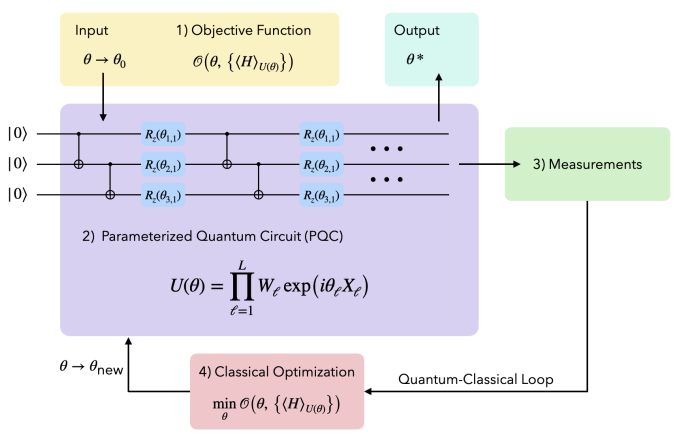
\includegraphics[scale=0.81]{./pics/vqa.png}
  \caption[The Variational Quantum Algorithm Structure]{The Variational Quantum Algorithm Structure~\cite{wang2024comprehensive}.}
  \label{fig:p10}
\end{figure}

\chapter{Proposed Solution}\vspace{-12pt}\label{solution}

In this chapter, the feasibility and potential of integrating quantum principles into Deep Learning Optimization are being presented. Specifically, neural hybrid architectures based on ODE (Ordinary Differential Equation)-inspired Quantum Visual Transformer (QViTs) network configurations are examined. Additionally, a generative Quantum Neural Network is designed, QRKT-GAN, leveraging qubits in varying quantities, from small to large. The primary aim of this thesis is not to tailor specific architectural components for particular problems in Computer Vision (CV) or Natural Language Processing (NLP). Instead, it focuses on experimenting with hybrid frameworks using widely recognized, consistent, and versatile datasets, complemented by robust classical optimization techniques.

To achieve this, the proposed ODE-QViTs networks are hybrid models that blend classical and Quantum Computing principles. These configurations aim to demonstrate how Quantum Mechanics can enhance the efficiency and performance of Deep Learning models. QRKT-GAN, the proposed generative Quantum Neural Network, leverages a Quantum Runge-Kutta method of 4th order within its architecture, aiming to explore the potential of Variational Quantum Circuits (VQC) in the context of ODEs.

The implementation leverages a variety of advanced technologies:

\begin{itemize}
  \item \textbf{JAX~\cite{bradbury2018jax} and Flax~\cite{heek2020flax}}: These are used for Just-In-Time (JIT) compilation and advanced numerical computing. They facilitate efficient computation with Deep Learning layers.
  \item \textbf{Tensorflow Quantum~\cite{broughton2020tensorflow}}: This tool provide a platform for building and training quantum models.
  \item \textbf{Qiskit~\cite{cross2018ibm}}: This is used for simulating and running quantum algorithms.
  \item \textbf{Pytorch~\cite{imambi2021pytorch}}: A popular deep learning framework that supports the implementation and training of complex neural networks.
  \item \textbf{Tensor Circuit~\cite{Zhang_2023}}: It is used for efficiently simulating Variational Quantum Circuits in a non-quantum environment leveraging Noisy Intermediate-Scale Quantum (NISQ) era.
\end{itemize}

Training the networks relies on strong classical techniques to ensure robustness and reliability in performance.

For the implementation of Quantum Visual Transformers Encoders and Unmasked Decoders, several key parameters are being considered~\cite{Comajoan_Cara_2024}:

\begin{itemize}
  \item \textbf{Patch Size}: Determines the size of the input data chunks.
  \item \textbf{Hidden Size}: Defines the dimensionality of the hidden layers within the transformer.
  \item \textbf{ODE-Transformer Blocks}: The design of these blocks is inspired by \cite{li2022ode}, integrating ODE principles into the transformer architecture.
  \item \textbf{Quantum Attention Heads}: These replace classical attention heads to leverage quantum parallelism.
  \item \textbf{Hidden QMLP Size}: Specifies the size of the hidden layers in the Quantum Multi-Layer Perceptron (QMLP).
\end{itemize}

These parameters are crucial for optimizing the QViTs architecture and ensuring it can effectively process and learn from the input data.

The QRKT-GAN generative hybrid network incorporates the following components:

\begin{itemize}
  \item \textbf{Generator and Discriminator Architectures}: Both are based on QViTs. The generator architecture specifically includes a  Quantum ODE lock, namely a Runge-Kutta 4th order one. This design is intended to investigate the utilization of VQCs in the context of ODEs.
\end{itemize}

The proposed model is shown below:

\begin{figure}[th]
  \centering
  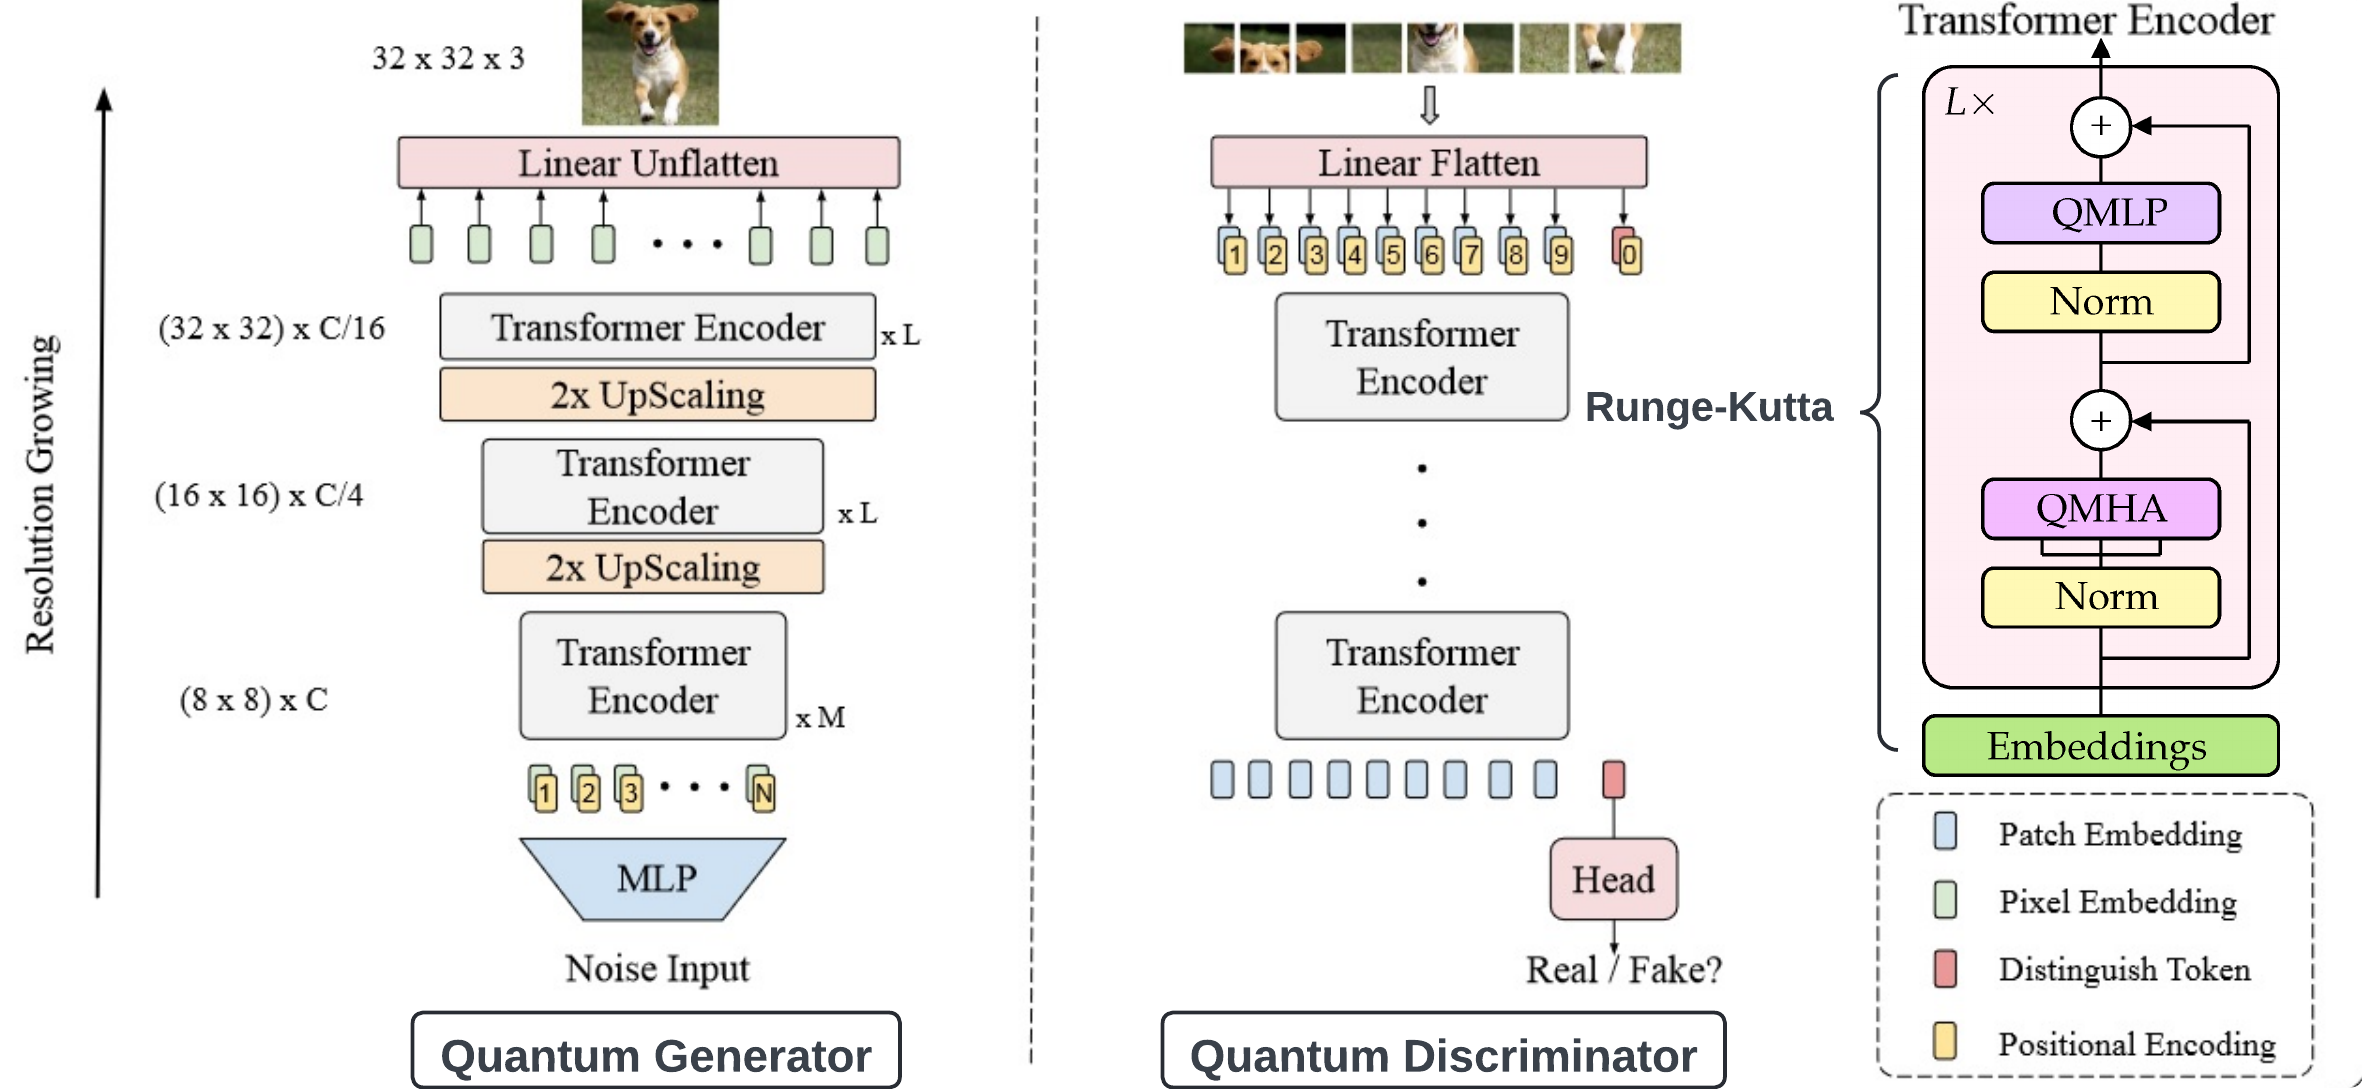
\includegraphics[scale=0.193]{./pics/Blank diagram - Page 1 (2).png}
  \caption[The QRKT-GAN Neural Architecture Structure]{The QRKT-GAN Neural Architecture Structure. Image inspired from~\cite{Comajoan_Cara_2024, jiang2021transgan}.}
  \label{fig:p11}
\end{figure}

The used Quantum Visual Transformer Neural Architecture is described as:
\\
\begin{figure}[th]
  \centering
  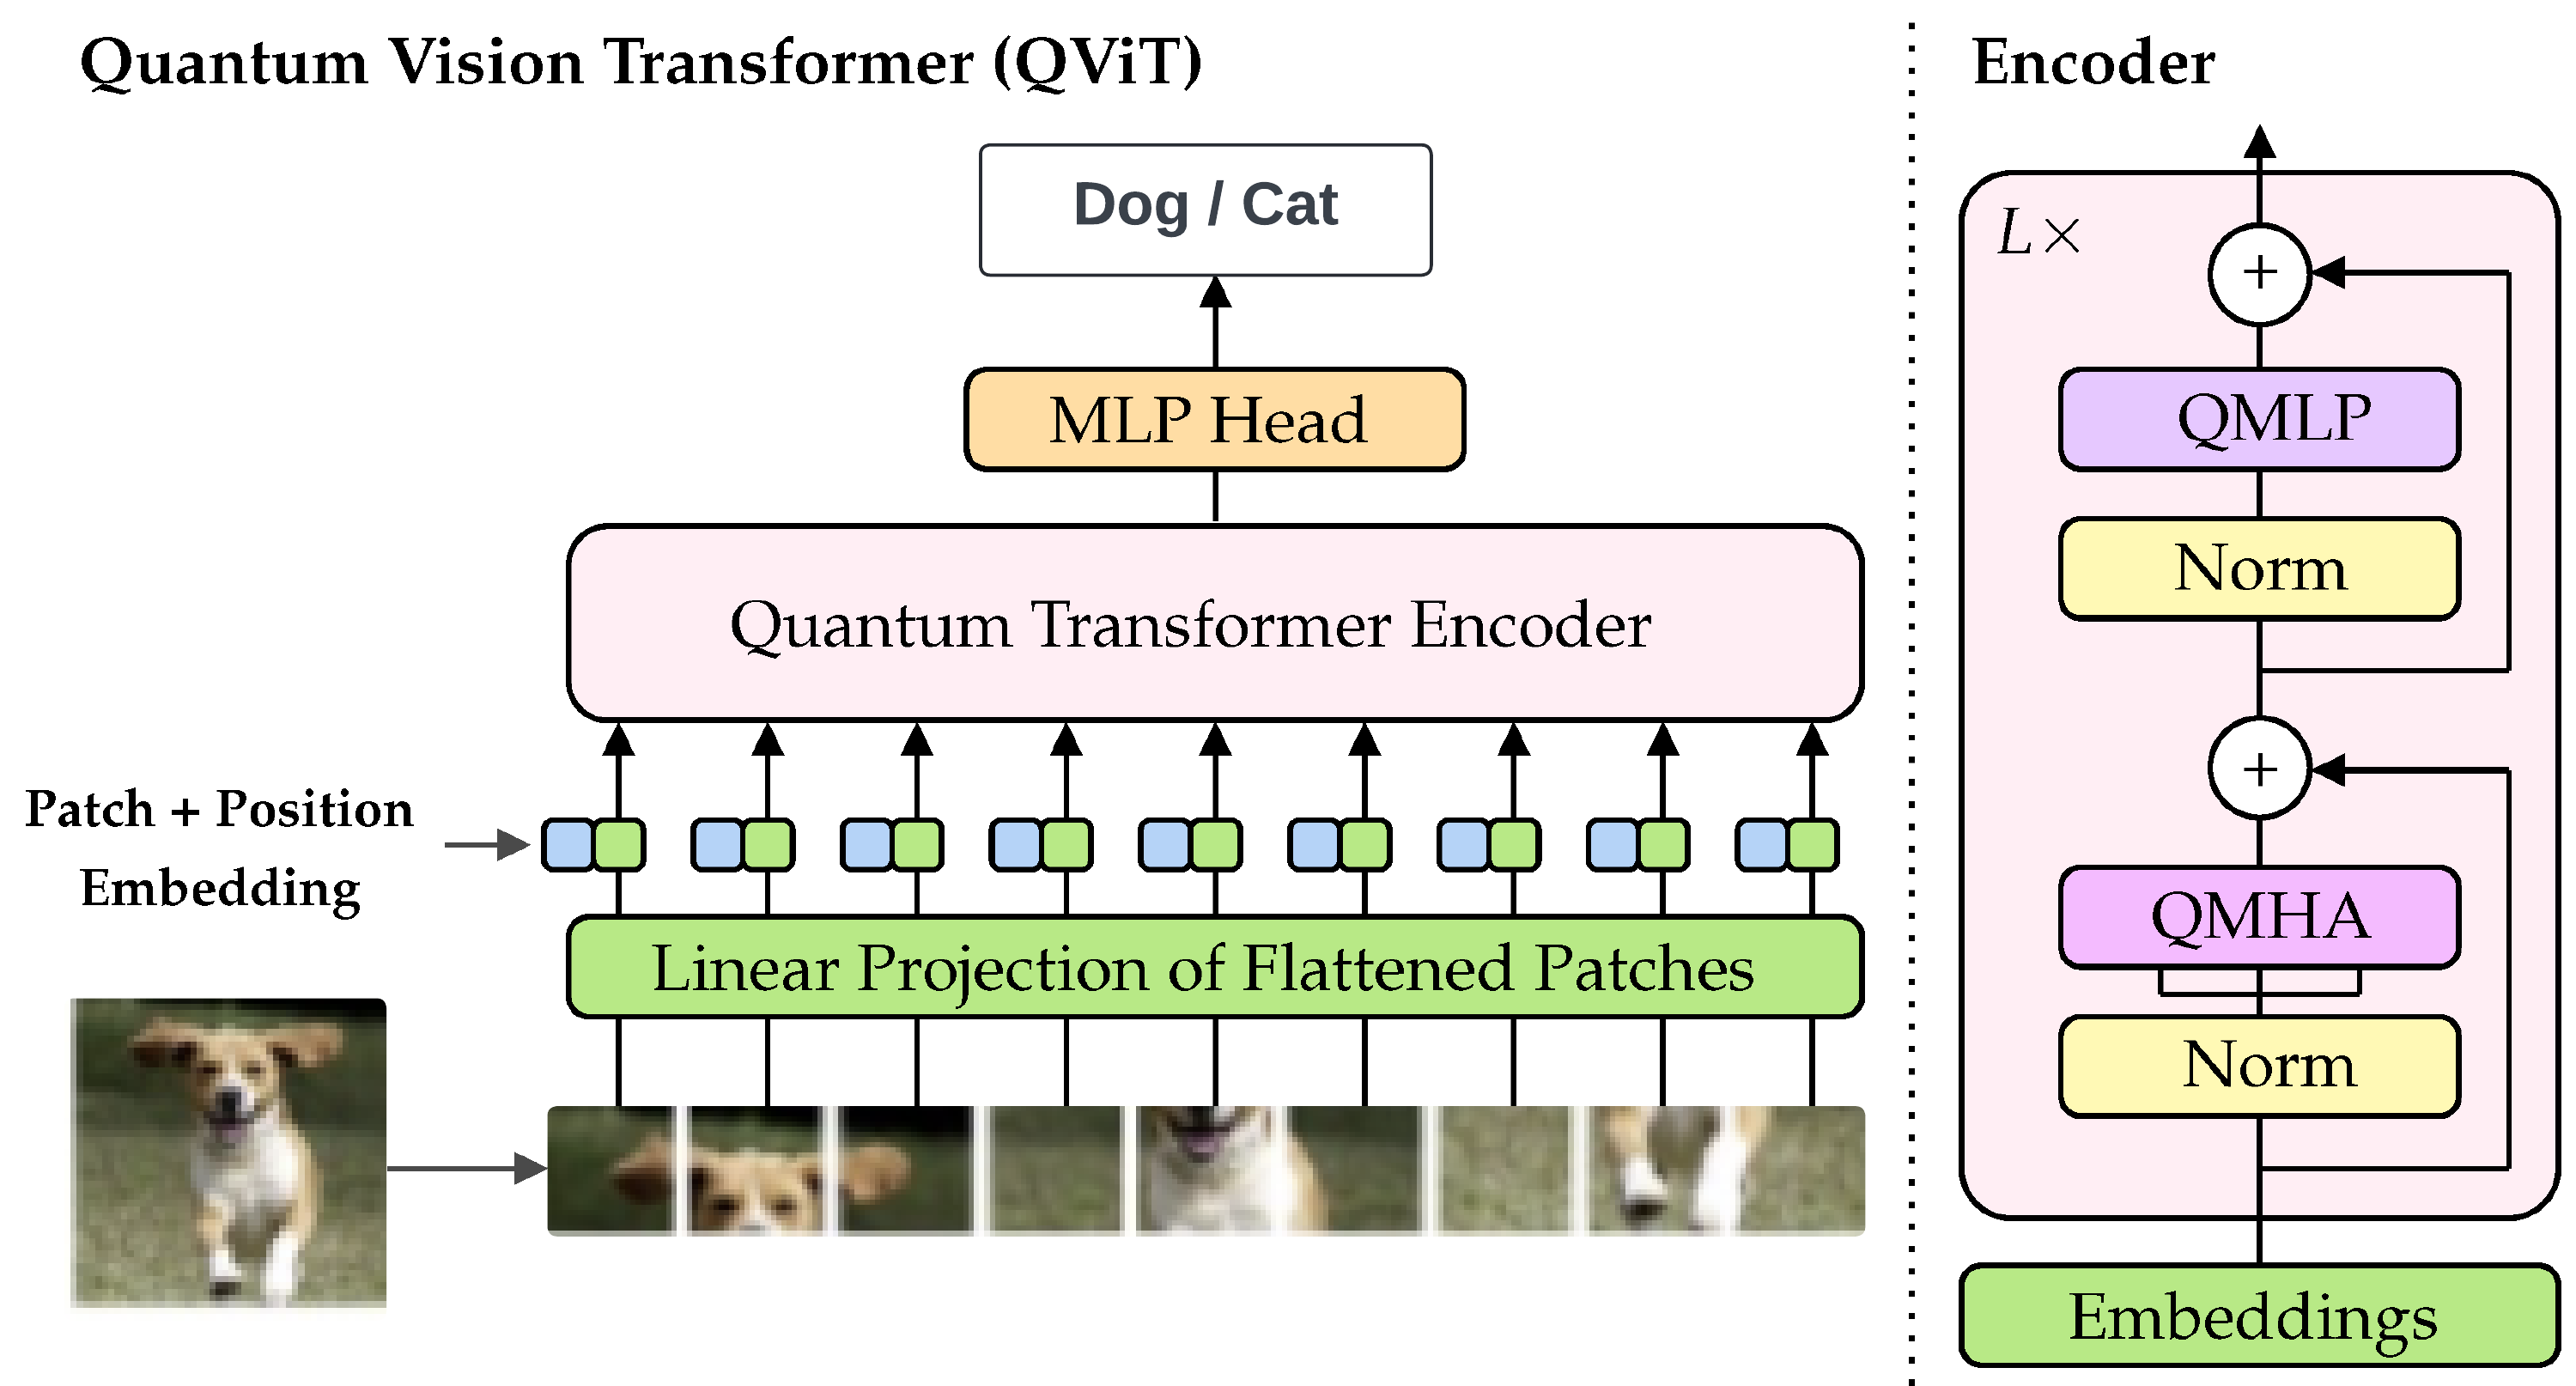
\includegraphics[scale=0.12]{./pics/Blank diagram - Page 1.png}
  \caption[The Quantum Visual Transformer used in QRKT-GAN]{The Quantum Visual Transformer used in QRKT-GAN. Image inspired from~\cite{Comajoan_Cara_2024}.}
  \label{fig:p12}
\end{figure}

And the VQC used for implementing the QMLP and Quantum Attention Heads is defined as:
\\
\begin{figure}[h]
  \[
    \begin{array}{c}
      \Qcircuit @C=0.75em @R=1.1em {
      \lstick{| \psi_0 \rangle}     & \gate{R_y(x_0)}     & \gate{R_x(\theta_0)}     & \gate{R_z(\theta_0)}     & \gate{H} & \ctrl{1} & \qw      & \qw      & \qw      & \qw      & \qw    & \qw      & \qw      & \qw      & \targ     & \meter \\
      \lstick{| \psi_1 \rangle}     & \gate{R_y(x_1)}     & \gate{R_x(\theta_1)}     & \gate{R_z(\theta_1)}     & \qw      & \targ    & \gate{H} & \ctrl{1} & \qw      & \qw      & \qw    & \qw      & \qw      & \qw      & \qw       & \meter \\
      \lstick{| \psi_2 \rangle}     & \gate{R_y(x_2)}     & \gate{R_x(\theta_2)}     & \gate{R_z(\theta_2)}     & \qw      & \qw      & \qw      & \targ    & \gate{H} & \ctrl{1} & \qw    & \qw      & \qw      & \qw      & \qw       & \meter \\
                                    & \vdots              & \vdots                   & \vdots                   &          &          &          &          &          & \vdots   & \vdots &          &          &          &           & \vdots \\
      \lstick{| \psi_{n-2} \rangle} & \gate{R_y(x_{n-2})} & \gate{R_x(\theta_{n-2})} & \gate{R_z(\theta_{n-2})} & \qw      & \qw      & \qw      & \qw      & \qw      & \qw      & \targ  & \gate{H} & \ctrl{1} & \qw      & \qw       & \meter \\
      \lstick{| \psi_{n-1} \rangle}     & \gate{R_y(x_{n-1})}     & \gate{R_x(\theta_{n-1})}     & \gate{R_z(\theta_{n-1})}     & \qw      & \qw      & \qw      & \qw      & \qw      & \qw      & \qw    & \qw      & \targ    & \gate{H} & \ctrl{-5} & \meter \\                                                                                                                            \\
      }
    \end{array}
  \]
  \caption{The Variational Quantum Circuit used in QRKT-GAN} \label{fig:vqc}
\end{figure}

Each component of the feature vector \( \mathbf{x} = (x_0, \ldots, x_{n-2}, x_{n-1}) \) is embedded into the quantum state of qubits by translating them into specific rotation angles. Following this, two layers of single-qubit rotations parameterized by \( \boldsymbol{\theta} = (\theta_0, \ldots, \theta_{n-2}, \theta_{n-1}) \) are applied to each qubit. These parameters, namely the qurons, are not static; they are optimized and learned alongside other model parameters during the training process.

In contrast with the Variational Quantum Circuit (VQC) from~\cite{Comajoan_Cara_2024}, the modified VQC presented here achieves a modest increase in accuracy, typically around 1-2\%. This improvement is attributed to the inclusion of additional \( R_y \), \( R_z \) and \( H \) gates. These gates are believed to enhance the circuit ability to capture information from the input features more effectively, allowing for a richer extraction of semantics from the patches.

The \( R_y \) gate is a rotation around the Y-axis of the Bloch sphere. It helps in adjusting the quantum state in a way that can represent the data more accurately.
The \( R_z \) gate is a rotation around the Z-axis of the Bloch sphere. It fine-tunes the phase of the quantum state, which can be crucial for encoding complex data patterns.
By incorporating these gates, the circuit can navigate the state space more freely and capture more nuanced features of the input data. This potentially leads to better learning and generalization.

The Hadamard gates are used to create superposition states, which are essential for quantum parallelism. They enable the circuit to consider multiple states simultaneously, thus increasing the computational efficiency.
These gates also facilitate the creation of Bell entangled states when combined with controlled-NOT (CNOT) gates. Entanglement is a unique quantum property that correlates the states of qubits, making it possible to represent more complex patterns and relationships within the data.
The entanglement helps in capturing deeper semantic relationships within the data patches, which traditional classical methods might miss. This can lead to a more robust and accurate model.

The added \( R_y \) and \( R_z \) gates, along with the Hadamard gates, likely contribute to the model improved performance through the following mechanisms:
\begin{itemize}
  \item \textbf{Enhanced Feature Representation:} The additional gates allow the quantum circuit to transform and represent the input data in a higher-dimensional space more effectively. This transformation helps in capturing more intricate patterns and features from the data.
  \item \textbf{Better Generalization:} The improved feature extraction and entanglement help the model generalize better to unseen data, reducing overfitting and improving accuracy.
  \item \textbf{Quantum Parallelism and Entanglement:} These quantum properties allow the model to explore multiple hypotheses simultaneously and capture complex dependencies within the data, which is often challenging for classical models.
\end{itemize}

The proposed enhancements to the VQC demonstrate a small but significant increase in accuracy, highlighting the potential benefits of leveraging additional quantum gates and entanglement in quantum circuits. The goal of QRKT-GAN is to generate realistic and high-quality synthetic data, leveraging the strengths of Quantum Computing to enhance generative models.

This chapter highlights the proposed hybrid architectural configurations, emphasizing their potential to integrate Quantum Computing principles into Deep Learning optimization. By using advanced technologies and innovative designs, such as ODE-based QViTs and QRKT-GAN, this research aims to push the boundaries of what is achievable in Deep Learning through the incorporation of Quantum Mechanics. The experiments will utilize popular and versatile datasets to validate the effectiveness of these hybrid models, showcasing their capability to address complex optimization problems in an energy-efficient manner.

\begin{figure}[th]
  \centering
  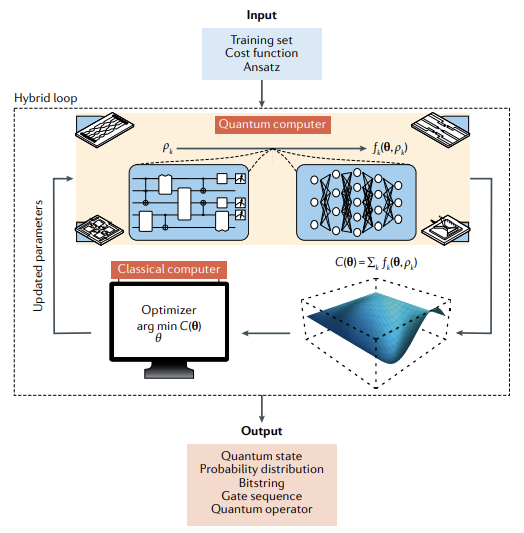
\includegraphics[scale=0.675]{./pics/image.png}
  \caption[Quantum Machine Learning Summary]{Quantum Machine Learning Summary~\cite{cerezo2021variational}}
  \label{fig:p13}
\end{figure}

\chapter{Experiments}\vspace{-12pt}
This chapter presents the methodologies used during the training and evaluation of the ODE models for classification tasks in computer vision (CV) and natural language processing (NLP) before the generation task. The datasets utilized in these experiments and the specific configurations of the QVits models are detailed. The final section of this chapter explores the generative capabilities of the QRKT-GAN compared to its classical baseline, TransGAN. All models are evaluated using consistent metrics, with an additional metric for the hybrid models: the number of qubits employed in learning the parameters of the qurons in the Variational Quantum Circuits (VQCs).

To begin with, the classification tasks in CV and NLP are approached using ODE models. These models were trained and evaluated on a range of benchmark datasets. For CV tasks, datasets such as MNIST and CIFAR-10 were used. For NLP task, IMDB for sentiment analysis was employed. Each dataset provided unique challenges and opportunities for the ODE models to demonstrate their robustness and adaptability. In terms of QVits configurations, various architectures were explored. The configurations varied in terms of the depth and width of the neural networks.

The generative capabilities of the QRKT-GAN is rigorously compared with the classical baseline TransGAN. The QRKT-GAN incorporates quantum-inspired techniques to enhance generative performance. The dataset used is CIFAR-10 for general object generation. Both models were evaluated based on standard generative metrics, such as Inception Score (IS) and Fréchet Inception Distance (FID).

An additional metric for the hybrid models is the number of qubits used in the VQCs. This metric is crucial as it provides insight into the quantum resource requirements for achieving specific performance levels. The evaluation highlighted that while QRKT-GAN required fewer parameters than TransGAN, it utilized a significant number of qubits, indicating a trade-off between classical and quantum resources.

Furthermore, classical and hybrid architectures are configured with a comparable number of components listed in chapter \ref{solution}. Given the fact that the input and output states of a Variational Quantum Circuit (VQC) share the same dimensions, the qubit count must match the size of the neural network corresponding layers. The designed and proposed VQC has $2n$ parameters compared to the classical fully connected layer $n^2 + n$ parameters.

The dimensions are kept minimal to limit qubit requirements, thereby reducing simulation time and enabling execution on current quantum hardware. A batch size of 65 is employed, with training spanning 65 epochs using the AdamW optimizer~\cite{zhang2018improved}, incorporating gradient clipping at norm 1, and a learning rate scheduler that transitions from a linear warmup over 5000 steps (0 to $10^{-3}$) to a cosine decay~\cite{learningrate2}. A random exhaustively hyperparameter search~\cite{randomsearch} is conducted to optimize parameters for the classical baseline, which are then applied to the QViT.

The classical components of the model, along with the classical baseline, are implemented and trained using JAX~\cite{bradbury2018jax} and Flax~\cite{heek2020flax,Comajoan_Cara_2024}. TensorCircuit~\cite{Zhang_2023} is utilized for the implementation, training, and execution of the VQCs via numerical simulation on a classical computer. This approach allows the quantum model to be trained for multiple epochs in a relatively decent duration. This represents a significant improvement over previous efforts, such as the work by Di Sipio et al.~\cite{di2022dawn}, which required around 100 hours to train a similar hybrid Transformer model for a single epoch, despite having a larger sample size.

\section{MNIST Digit Classification}
The MNIST~\cite{lecun2010mnist} dataset is a large database of handwritten digits commonly used for training various Image Processing systems. This consistent dataset contains 60,000 training images and 10,000 testing images, each of which is a 28x28 grayscale image of a single digit from 0 to 9. MNIST serves as a standard benchmark in Machine Learning due to its simplicity and the ease with which models can achieve high accuracy. It is particularly useful for validating new algorithms and models.

In this experiment, the dataset is strategically divided into three distinct parts to ensure comprehensive model evaluation and optimization. The training split, containing 54,000 images, provides a robust foundation for the model to learn diverse patterns and features. For hyperparameter tuning and model refinement, a validation split of 6,000 images is used during the Random Search process. This helps in selecting the best-performing model configuration. Lastly, to rigorously test the model generalization capability, 10,000 images are reserved in the test set, which remains unseen during the training phase. This approach ensures that the model is not only well-trained but also performs effectively on new, unseen data, reflecting its true predictive power.

Some extracted samples are shown below:

\begin{figure}[th]
  \centering
  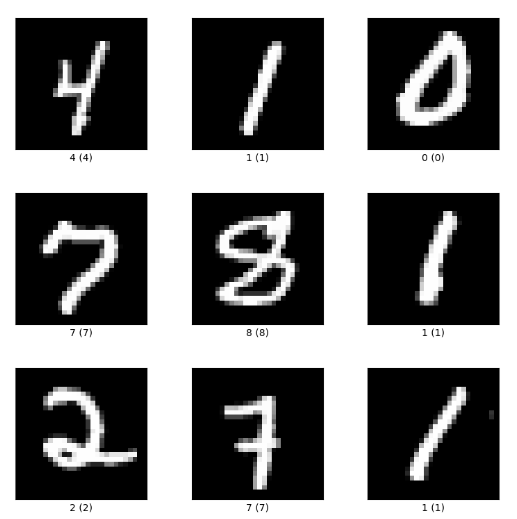
\includegraphics[scale=0.65]{./pics/mnist.png}
  \caption[Examples from MNIST]{Examples from MNIST\protect\footnotemark}
  \label{fig:p14}
\end{figure}
\footnotetext{\url{https://www.tensorflow.org/datasets/catalog/mnist}}

The progress of the AUC and the loss using \textbf{one classical ODE block}-based network, calculated at every epoch, is here:

\begin{figure}[th]
  \centering
  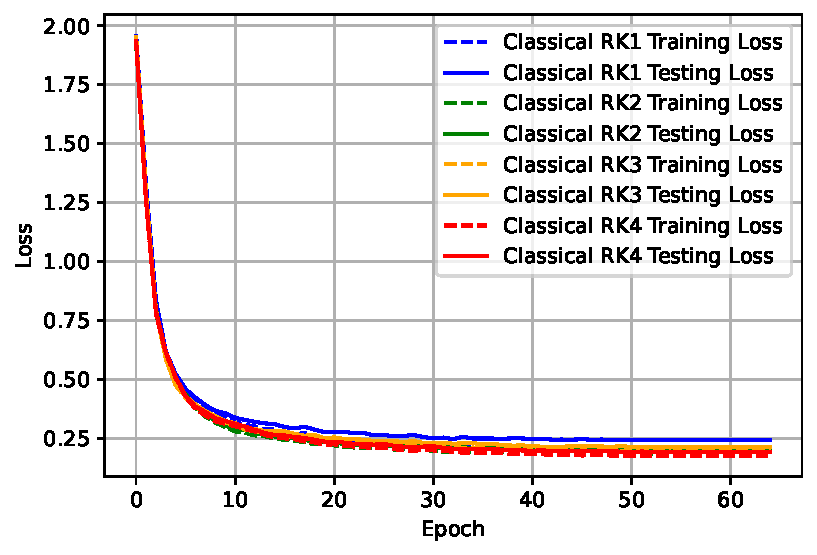
\includegraphics[scale=0.88]{./pics/new_pdf_graphs/classical/3_enc_1_rk_1_dec/classical_transfomer_loss_mnist_rk1_rk2_rk3_rk4.pdf}
  \caption[Cross-entropy loss evolution during learning]{Cross-entropy loss evolution during learning}
  \label{fig:p15}
  \vspace*{\floatsep}
  \centering
  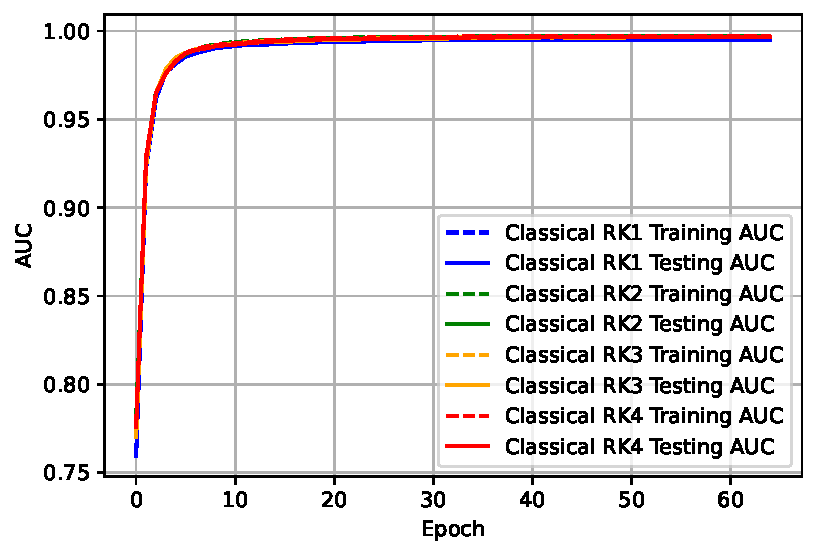
\includegraphics[scale=0.88]{./pics/new_pdf_graphs/classical/3_enc_1_rk_1_dec/classical_transfomer_auc_mnist_rk1_rk2_rk3_rk4.pdf}
  \caption[AUC score evolution during learning]{AUC score evolution during learning}
  \label{fig:p16}
\end{figure}

This implementation showcases the following components and parameters:
\begin{itemize}
  \item \textbf{Patch Size}: 14
  \item \textbf{Hidden Size}: 6
  \item \textbf{Classical ODE-Transformer Blocks}: 1
  \item \textbf{Classical Attention Heads}: 2
  \item \textbf{Hidden MLP Size}: 3
\end{itemize}

\begin{table}[th]\small\linespread{1}
  \label{tab:classical_MNIST_0}
  \centering
  \begin{tabular}{|l|c|c|c|c|c|c|}
    \hline
    \textbf{ODE} & \textbf{Train Time (s)} & \textbf{Accuracy} & \textbf{F1 Score} & \textbf{Best AUC Epoch} & \textbf{\# Parameters} & \textbf{\# Qubits} \\
    \hline
    RK1          & 1544.82                 & 94\%              & 93\%              & 50                      & 3733                   & -                  \\
    RK2          & 1524.14                 & 94\%              & 94\%              & 55                      & 3946                   & -                  \\
    RK3          & 1539.63                 & 94\%              & 94\%              & 51                      & 4159                   & -                  \\
    RK4          & 1560.66                 & 95\%              & 94\%              & 51                      & 4372                   & -                  \\
    \hline
  \end{tabular}
  \caption{MNIST metrics for the classical baselines}
\end{table}

Observations:

The F1 Scores are consistently high across all models, with RK1 scoring slightly lower at 93\%. RK2, RK3, and RK4 all achieve a 94\% F1 Score, indicating a good balance between precision and recall for these models.

The epoch at which the best Area Under the Curve (AUC) is achieved varies slightly. RK2 reaches its best AUC performance at epoch 55, which is higher than the others. RK1 achieves its best AUC at epoch 50, while RK3 and RK4 both reach their best performance at epoch 51.

The number of parameters increases progressively from RK1 to RK4. RK1 has the fewest parameters at 3733, while RK4 has the most at 4372. This indicates that RK4 is a more complex model compared to the others, which may contribute to its slightly better performance metrics.

\clearpage

And between the optimized RK4 and traditional RK4:

\begin{figure}[th]
  \centering
  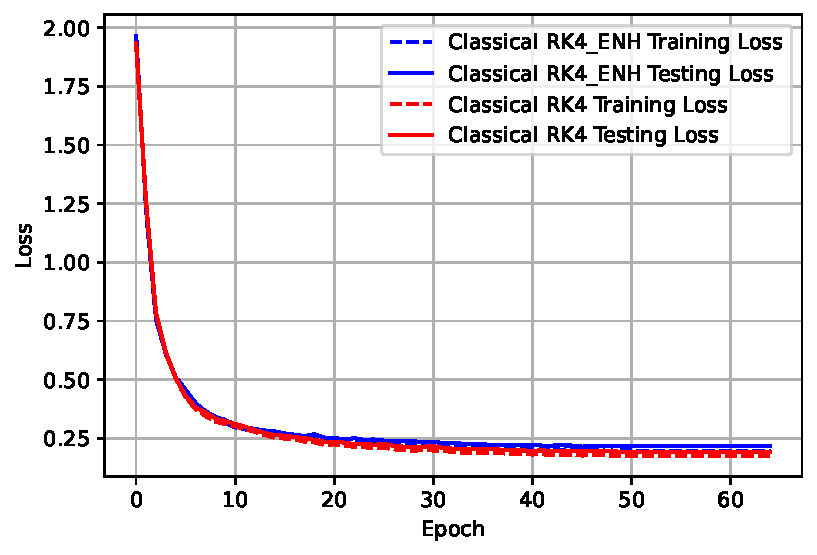
\includegraphics[scale=0.88]{./pics/new_pdf_graphs/classical/3_enc_1_rk_1_dec/classical_transfomer_loss_mnist_rk4_rk4_enh.pdf}
  \caption[Cross-entropy loss evolution during learning]{Cross-entropy loss evolution during learning}
  \label{fig:p17}
  \vspace*{\floatsep}
  \centering
  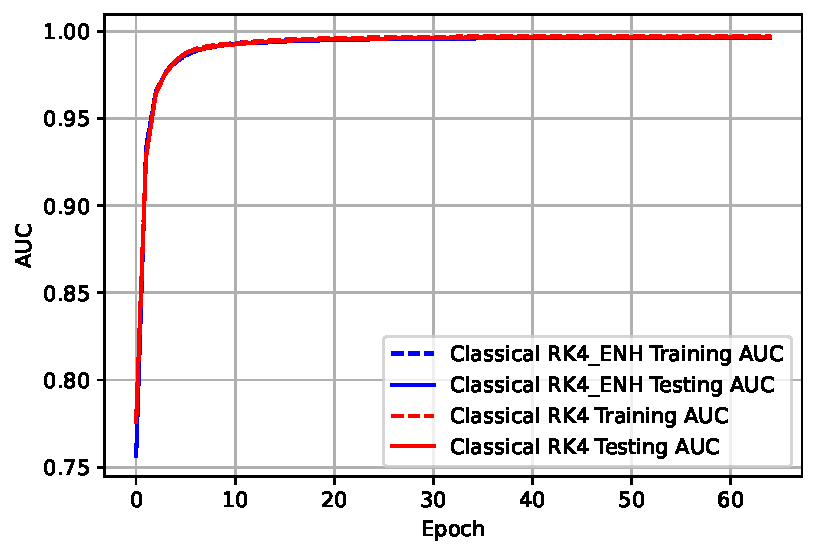
\includegraphics[scale=0.88]{./pics/new_pdf_graphs/classical/3_enc_1_rk_1_dec/classical_transfomer_auc_mnist_rk4_rk4_enh.pdf}
  \caption[AUC score evolution during learning]{AUC score evolution during learning}
  \label{fig:p18}
\end{figure}


For the MNIST classification task, the optimized variant does not demonstrate any significant improvement in training loss, testing loss, or AUC. This lack of impact could be attributed to the relatively small dimensionality of the problem, where further adjustments yield negligible effects. Consequently, the inherent simplicity of the dataset may limit the benefits of optimization techniques.

\clearpage

\begin{table}[th]\small\linespread{1}
  \label{tab:classical_MNIST_1}
  \centering
  \begin{tabular}{|l|c|c|c|c|c|c|}
    \hline
    \textbf{ODE} & \textbf{Train Time (s)} & \textbf{Accuracy} & \textbf{F1 Score} & \textbf{Best AUC Epoch} & \textbf{\# Parameters} & \textbf{\# Qubits} \\
    \hline
    RK4          & 1560.66                 & 95\%              & 94\%              & 51                      & 4372                   & -                  \\
    RK4\_ENH     & 1562.54                 & 94\%              & 94\%              & 49                      & 4372                   & -                  \\
    \hline
  \end{tabular}
  \caption{MNIST metrics for the classical baselines}
\end{table}

Observations:

The training times for RK4 and RK4\_ENH are very close, with RK4\_ENH taking slightly longer. This suggests that the enhancements in RK4\_ENH do not significantly increase the training time, making it comparable in terms of computational requirements.

RK4 achieves a slightly higher accuracy of 95\% compared to 94\% for RK4\_ENH. This indicates that the base RK4 model is marginally better at correctly classifying the MNIST dataset images.

Both models have an identical F1 Score of 94\%, demonstrating a consistent balance between precision and recall. This suggests that the enhancement does not significantly affect the F1 Score.

RK4 reaches its best AUC at epoch 51, whereas RK4\_ENH reaches it at epoch 49. This slight difference indicates that RK4\_ENH achieves its optimal performance slightly earlier in the training process compared to RK4.

Both models have the same number of parameters, indicating that the enhancements in RK4\_ENH do not involve changes in the model complexity or size.

\clearpage

The progress of the AUC and the loss using \textbf{three classical ODE blocks}-based network, calculated at every epoch, is here:

\begin{figure}[th]
  \centering
  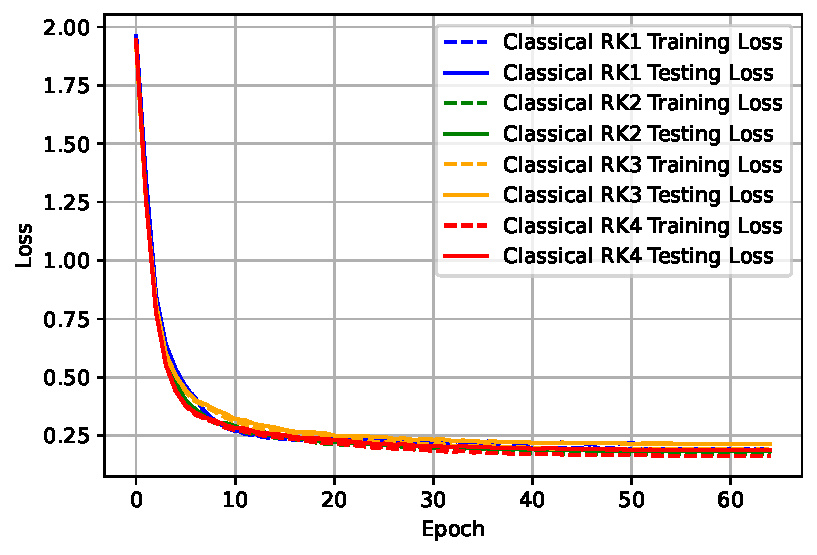
\includegraphics[scale=0.88]{./pics/new_pdf_graphs/classical/3_rk_1_dec/classical_transfomer_loss_mnist_rk1_rk2_rk3_rk4.pdf}
  \caption[Cross-entropy loss evolution during learning]{Cross-entropy loss evolution during learning}
  \label{fig:p19}
  \vspace*{\floatsep}
  \centering
  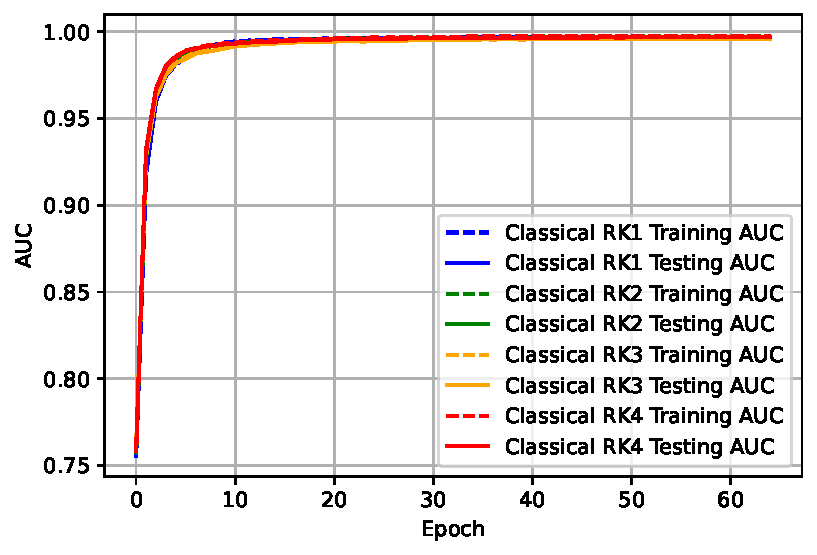
\includegraphics[scale=0.88]{./pics/new_pdf_graphs/classical/3_rk_1_dec/classical_transfomer_auc_mnist_rk1_rk2_rk3_rk4.pdf}
  \caption[AUC score evolution during learning]{AUC score evolution during learning}
  \label{fig:p20}
\end{figure}

This implementation showcases the following components and parameters:
\begin{itemize}
  \item \textbf{Patch Size}: 14
  \item \textbf{Hidden Size}: 6
  \item \textbf{Classical ODE-Transformer Blocks}: 3
  \item \textbf{Classical Attention Heads}: 2
  \item \textbf{Hidden MLP Size}: 3
\end{itemize}

\begin{table}[th]\small\linespread{1}
  \label{tab:classical_MNIST_3}
  \centering
  \begin{tabular}{|l|c|c|c|c|c|c|}
    \hline
    \textbf{ODE} & \textbf{Train Time (s)} & \textbf{Accuracy} & \textbf{F1 Score} & \textbf{Best AUC Epoch} & \textbf{\# Parameters} & \textbf{\# Qubits} \\
    \hline
    RK1          & 1582.73                 & 94\%              & 94\%              & 50                      & 3472                   & -                  \\
    RK2          & 1689.24                 & 95\%              & 95\%              & 53                      & 4693                   & -                  \\
    RK3          & 1850.70                 & 94\%              & 94\%              & 55                      & 5332                   & -                  \\
    RK4          & 1925.89                 & 95\%              & 95\%              & 51                      & 5971                   & -                  \\
    \hline
  \end{tabular}
  \caption{MNIST metrics for the classical baselines}
\end{table}

Observations:

Both RK2 and RK4 achieve the highest scores, demonstrating that higher-order methods can offer slight improvements in classification performance.

RK1 and RK3 both achieve an accuracy and F1 score of 94\%, which is marginally lower than RK2 and RK4. This suggests that while all methods are effective, the second and fourth-order methods have a slight edge in performance.

Training time increases with the order of the Runge-Kutta method. RK1, being the simplest and least computationally intensive method, has the shortest training time. As the order increases, so does the complexity and the computational load, resulting in longer training times: RK2, RK3, and RK4.

The epoch at which the model achieves its best Area Under the Curve (AUC) varies slightly among the methods. RK1 and RK4 reach their peak AUC at around 50 and 51 epochs respectively, while RK2 and RK3 reach it slightly later at 53 and 55 epochs.

More complex methods involve more parameters, which can contribute to improved performance but also add to the model complexity and training time.

\clearpage

And between the optimized RK4 and traditional RK4:

\begin{figure}[th]
  \centering
  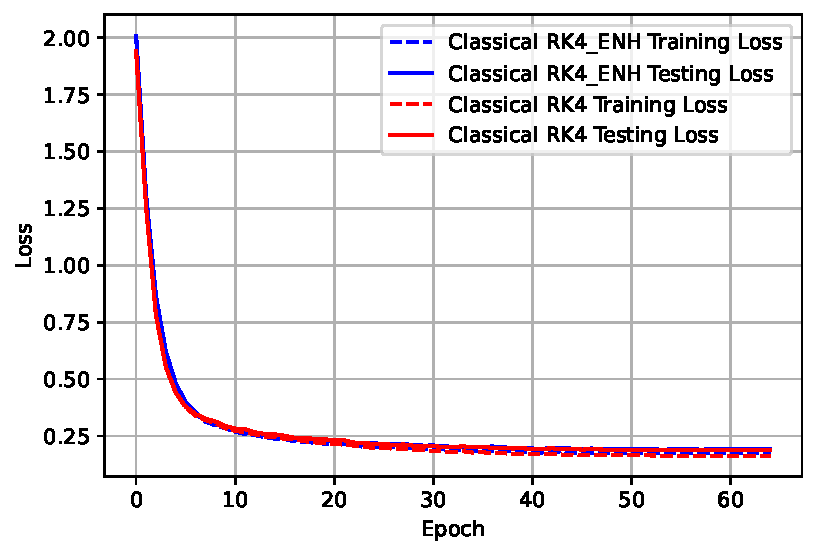
\includegraphics[scale=0.88]{./pics/new_pdf_graphs/classical/3_rk_1_dec/classical_transfomer_loss_mnist_rk4_rk4_enh.pdf}
  \caption[Cross-entropy loss evolution during learning]{Cross-entropy loss evolution during learning}
  \label{fig:p21_}
  \vspace*{\floatsep}
  \centering
  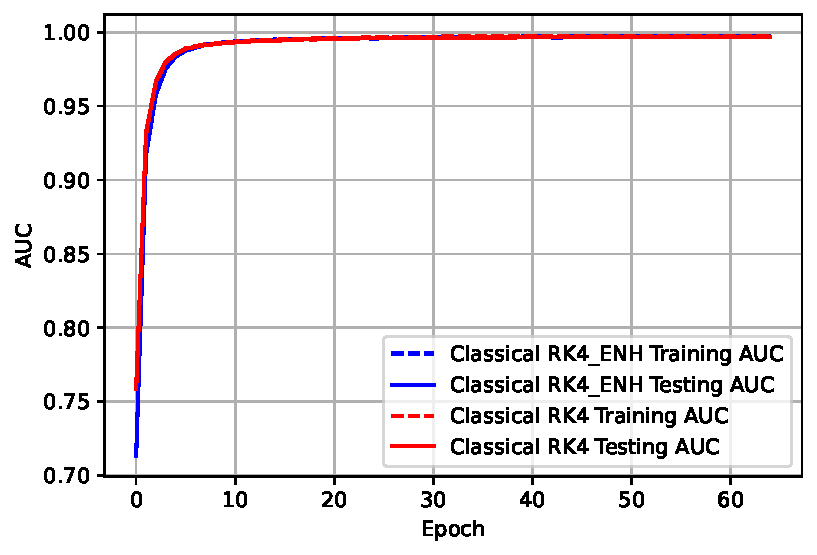
\includegraphics[scale=0.88]{./pics/new_pdf_graphs/classical/3_rk_1_dec/classical_transfomer_auc_mnist_rk4_rk4_enh.pdf}
  \caption[AUC score evolution during learning]{AUC score evolution during learning}
  \label{fig:p21}
\end{figure}


Like before, The optimized variant does not show any significant improvement in training loss, testing loss, or AUC. This lack of impact could be due to the relatively small dimensionality of the problem, where further adjustments have minimal effects. Consequently, the inherent simplicity of the dataset may limit the advantages of optimization techniques.
\clearpage

\begin{table}[th]\small\linespread{1}
  \label{tab:classical_MNIST_2}
  \centering
  \begin{tabular}{|l|c|c|c|c|c|c|}
    \hline
    \textbf{ODE} & \textbf{Train Time (s)} & \textbf{Accuracy} & \textbf{F1 Score} & \textbf{Best AUC Epoch} & \textbf{\# Parameters} & \textbf{\# Qubits} \\
    \hline
    RK4          & 1925.89                 & 95\%              & 95\%              & 51                      & 5971                   & -                  \\
    RK4\_ENH     & 1842.04                 & 95\%              & 95\%              & 54                      & 5971                   & -                  \\
    \hline
  \end{tabular}
  \caption{MNIST metrics for the classical baselines}
\end{table}

Observations:

The training time for the enhanced RK4 method is slightly less than the standard RK4, suggesting improved computational efficiency.

Both RK4 and RK4\_ENH achieve an accuracy of 95\%, indicating that the enhancement does not compromise the classification performance.

Both methods achieve an F1 score of 95\%, reaffirming that the enhancement maintains the model ability to balance precision and recall.

The enhanced model reaches its peak AUC slightly later, at the 54th epoch. This might indicate a different learning curve or optimization process.

These methods have the same number of parameters, indicating that the enhancement does not involve increasing the model complexity in terms of parameters.

\clearpage
The progress of the AUC and the loss using \textbf{three ODE quantum blocks}-based network, calculated at every epoch, is here:

\begin{figure}[th]
  \centering
  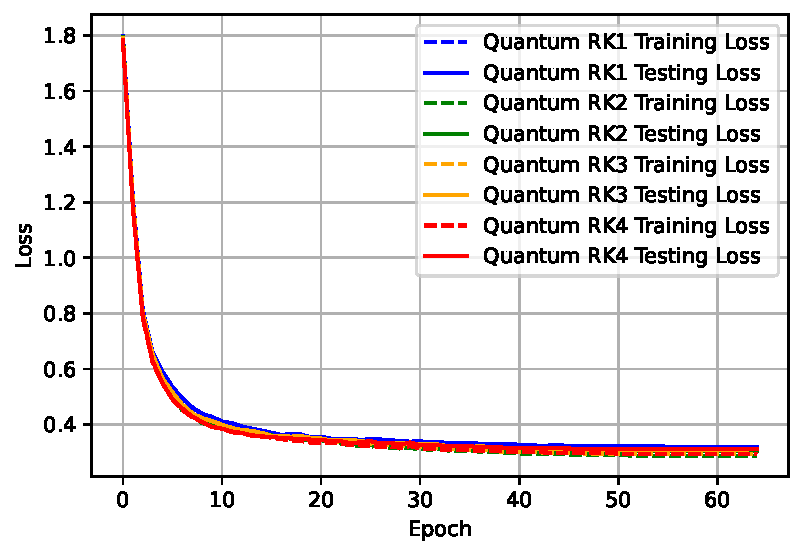
\includegraphics[scale=0.88]{./pics/new_pdf_graphs/quantum/3_rk_1_dec/quantum_transfomer_loss_mnist_rk1_rk2_rk3_rk4.pdf}
  \caption[Cross-entropy loss evolution during learning]{Cross-entropy loss evolution during learning}
  \label{fig:p22}
  \vspace*{\floatsep}
  \centering
  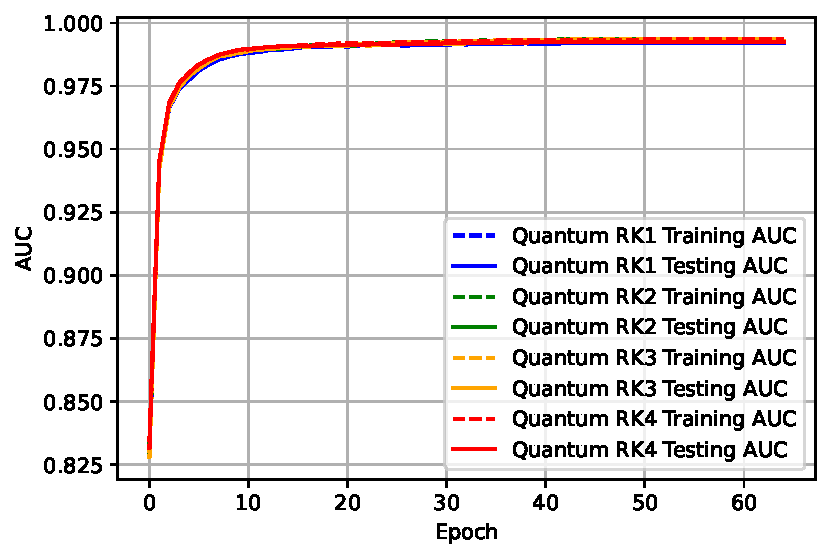
\includegraphics[scale=0.88]{./pics/new_pdf_graphs/quantum/3_rk_1_dec/quantum_transfomer_auc_mnist_rk1_rk2_rk3_rk4.pdf}
  \caption[AUC score evolution during learning]{AUC score evolution during learning}
  \label{fig:p23}
\end{figure}

This implementation showcases the following components and parameters:
\begin{itemize}
  \item \textbf{Patch Size}: 14
  \item \textbf{Hidden Size}: 6
  \item \textbf{Quantum ODE-Transformer Blocks}: 3
  \item \textbf{Quantum Attention Heads}: 2
  \item \textbf{Hidden QMLP Size}: 3
\end{itemize}

\begin{table}[th]\small\linespread{1}
  \label{tab:classical_MNIST_3}
  \centering
  \begin{tabular}{|l|c|c|c|c|c|c|}
    \hline
    \textbf{ODE} & \textbf{Train Time (s)} & \textbf{Accuracy} & \textbf{F1 Score} & \textbf{Best AUC Epoch} & \textbf{\# Parameters} & \textbf{\# Qubits} \\
    \hline
    QRK1         & 2051.72                 & 91\%              & 91\%              & 56                      & 2872                   & 114                \\
    QRK2         & 2442.47                 & 91\%              & 91\%              & 47                      & 3088                   & 195                \\
    QRK3         & 2945.24                 & 91\%              & 91\%              & 52                      & 3304                   & 276                \\
    QRK4         & 3594.99                 & 91\%              & 91\%              & 52                      & 3520                   & 357                \\
    \hline
  \end{tabular}
  \caption{MNIST metrics for the quantum configurations}
\end{table}

Observations:

Training time increases with the order of the quantum Runge-Kutta method, reflecting the increasing computational complexity.

All quantum methods achieve an accuracy of 91\%. This consistency suggests that the order of the method does not significantly impact accuracy in the quantum implementations.

Similar to accuracy, the F1 score is 91\% for all quantum methods, indicating consistent performance in balancing precision and recall.

The best AUC epoch varies, with QRK2 reaching its peak performance earliest at 47 epochs, while QRK1 reaches it the latest at 56 epochs.

The number of parameters increases with the order of the method, which is expected as higher-order methods typically involve more complex calculations.

Higher-order methods require significantly more qubits, indicating a substantial increase in quantum resource requirements.

\clearpage

And between the optimized RK4 and traditional RK4:

\begin{figure}[th]
  \centering
  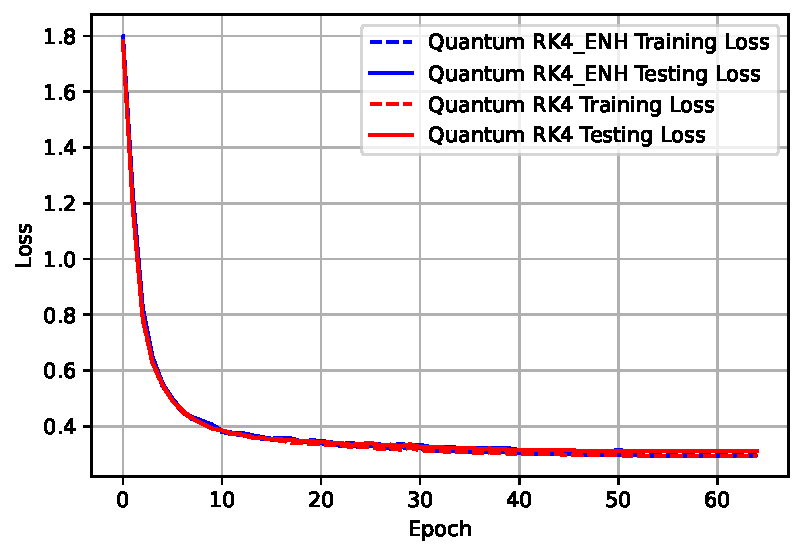
\includegraphics[scale=0.88]{./pics/new_pdf_graphs/quantum/3_rk_1_dec/quantum_transfomer_loss_mnist_rk4_rk4_enh.pdf}
  \caption[Cross-entropy loss evolution during learning]{Cross-entropy loss evolution during learning}
  \label{fig:p24}
  \vspace*{\floatsep}
  \centering
  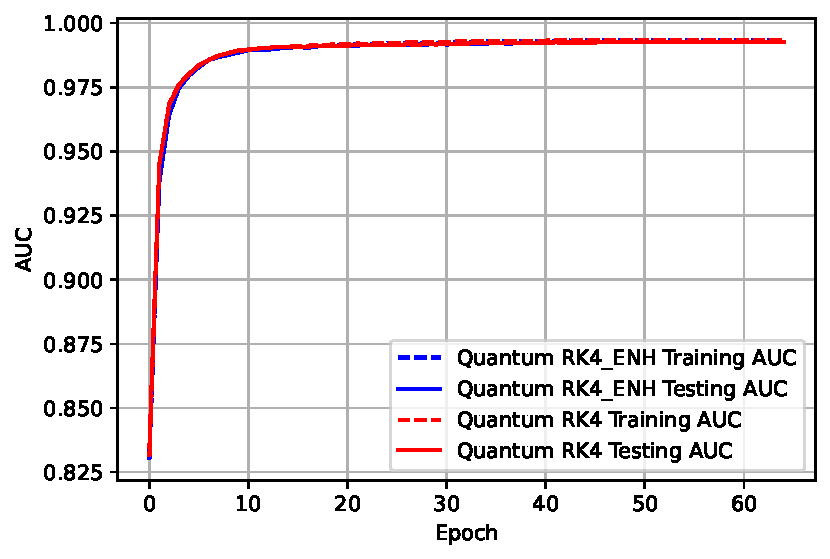
\includegraphics[scale=0.88]{./pics/new_pdf_graphs/quantum/3_rk_1_dec/quantum_transfomer_auc_mnist_rk4_rk4_enh.pdf}
  \caption[AUC score evolution during learning]{AUC score evolution during learning}
  \label{fig:p25}
\end{figure}


Similar to previous observations, the optimized variant fails to exhibit significant improvements in training loss, testing loss, or AUC. This lack of noticeable impact might stem from the relatively small dimensionality of the problem, where further adjustments produce negligible effects. As a result, the inherent simplicity of the dataset may constrain the potential benefits of optimization techniques.
\clearpage

\begin{table}[th]\small\linespread{1}
  \label{tab:classical_MNIST_3}
  \centering
  \begin{tabular}{|l|c|c|c|c|c|c|}
    \hline
    \textbf{ODE} & \textbf{Train Time (s)} & \textbf{Accuracy} & \textbf{F1 Score} & \textbf{Best AUC Epoch} & \textbf{\# Parameters} & \textbf{\# Qubits} \\
    \hline
    QRK4         & 3594.99                 & 91\%              & 91\%              & 52                      & 3520                   & 357                \\
    QRK4\_ENH    & 3539.44                 & 91\%              & 91\%              & 48                      & 3520                   & 357                \\
    \hline
  \end{tabular}
  \caption{MNIST metrics for the quantum configurations}
\end{table}

Observations:

The enhanced QRK4 method has a slightly reduced training time, suggesting improved computational efficiency.

Both QRK4 and QRK4\_ENH achieve an accuracy of 91\%, indicating that the enhancement does not impact the classification performance negatively.

Both methods have an F1 score of 91\%, which means the enhanced method maintains the same balance between precision and recall as the standard method.

The enhanced model reaches its peak AUC earlier, at the 48th epoch, indicating potentially faster convergence.

Both methods have the same number of parameters, suggesting that the enhancement does not involve increasing the model complexity in terms of parameters.

Both methods require the same number of qubits, indicating that the enhancement does not increase quantum resource requirements.

\clearpage
The progress of the AUC and the loss using \textbf{three ODE quantum and classical blocks}-based network, calculated at every epoch, is here:

\begin{figure}[th]
  \centering
  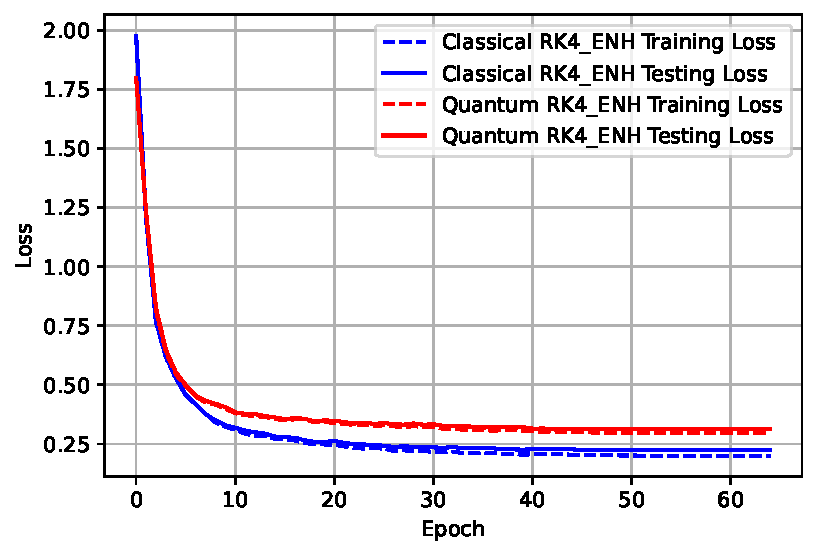
\includegraphics[scale=0.88]{./pics/new_pdf_graphs/hybrid/alternative_hybrid_transfomer_loss_mnist_rk4_enh.pdf}
  \caption[Cross-entropy loss evolution during learning]{Cross-entropy loss evolution during learning}
  \label{fig:p26}
  \vspace*{\floatsep}
  \centering
  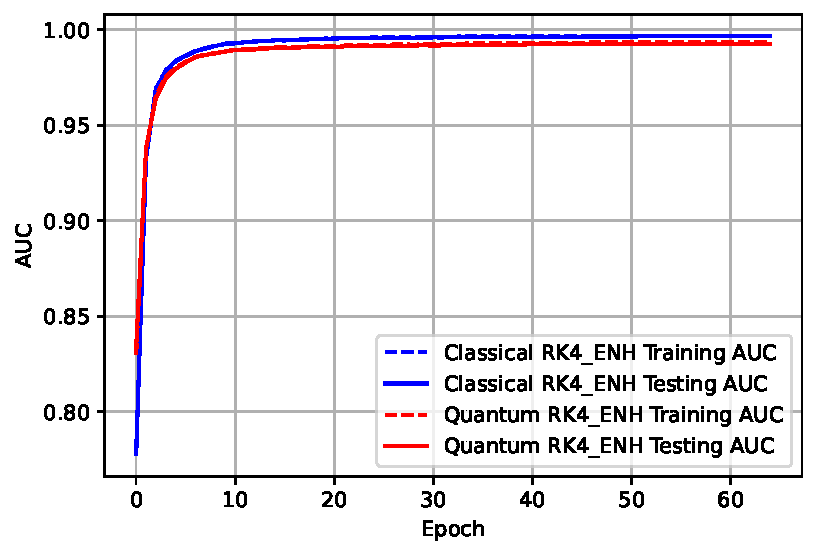
\includegraphics[scale=0.88]{./pics/new_pdf_graphs/hybrid/hybrid_auc_mnist_rk4.pdf}
  \caption[AUC score evolution during learning]{AUC score evolution during learning}
  \label{fig:p27}
\end{figure}

This implementation showcases the following components and parameters:
\begin{itemize}
  \item \textbf{Patch Size}: 14
  \item \textbf{Hidden Size}: 6
  \item \textbf{Classical and Quantum ODE-Transformer Blocks}: 3
  \item \textbf{Classical and Quantum Attention Heads}: 2
  \item \textbf{Hidden QMLP Size}: 3
\end{itemize}


\clearpage

\begin{table}[th]\small\linespread{1}
  \label{tab:hybrid_MNIST}
  \centering
  \begin{tabular}{|l|c|c|c|c|c|c|}
    \hline
    \textbf{ODE} & \textbf{Train Time (s)} & \textbf{Accuracy} & \textbf{F1 Score} & \textbf{Best AUC Epoch} & \textbf{\# Parameters} & \textbf{\# Qubits} \\
    \hline
    RK4\_ENH     & 1842.04                 & 95\%              & 95\%              & 54                      & 5971                   & -                  \\
    QRK4\_ENH    & 3539.44                 & 91\%              & 91\%              & 48                      & 3520                   & 357                \\
    \hline
  \end{tabular}
  \caption{MNIST metrics for the quantum and classical configurations}
\end{table}

Observations:

The training time for the enhanced quantum QRK4 method is significantly longer than the classical method.

The accuracy of the enhanced quantum method is lower compared to the classical method.

The F1 score of the enhanced quantum method is consistent with its accuracy, indicating a balanced precision and recall.

The enhanced quantum method achieves its best AUC performance earlier, suggesting faster convergence.

The quantum method has fewer parameters, indicating potentially lower model complexity.

\clearpage

\section{CIFAR-10 Object Classification}

CIFAR-10 is another widely used dataset in the field of Computer Vision. It consists of 60,000 32x32 color images in 10 different classes, with 6,000 images per class. The classes include airplanes, cars, birds, cats, deer, dogs, etc. The dataset is divided into 50,000 training images and 10,000 testing images. CIFAR-10 is more complex than MNIST due to its color images and diverse range of object classes, making it a suitable challenge for evaluating the performance of more advanced models.

In this experiment, the dataset is meticulously divided into three distinct segments to ensure thorough model evaluation and optimization. The training split, comprising 45,000 images, offers a solid foundation for the model to learn diverse patterns and features. A validation split of 5,000 images is employed during the Random Search process for hyperparameter tuning and model refinement, facilitating the selection of the best-performing model configuration. Finally, to rigorously assess the model generalization capability, 10,000 images are set aside in the test set, remaining unseen during the training phase. This method ensures that the model is not only well-trained but also demonstrates effective performance on new, unseen data, accurately reflecting its true predictive power.

Some extracted samples are shown below:

\begin{figure}[th]
  \centering
  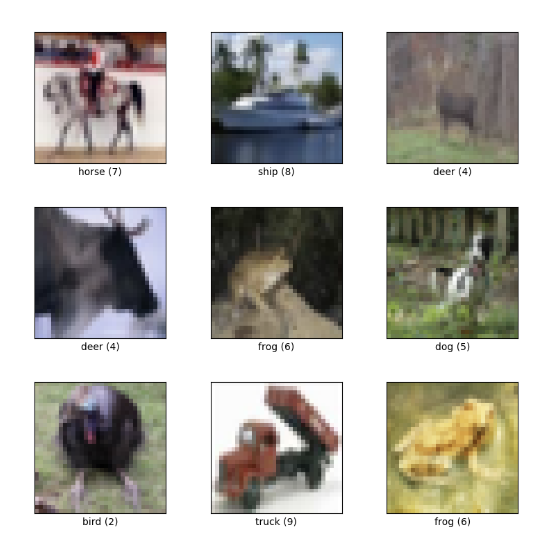
\includegraphics[scale=0.75]{./pics/cifar10.png}
  \caption[Examples from CIFAR-10]{Examples from CIFAR-10\protect\footnotemark}
  \label{fig:p28}
\end{figure}
\footnotetext{\url{https://www.tensorflow.org/datasets/catalog/cifar10}}

\clearpage

The progress of the AUC and the loss using \textbf{one classical ODE block}-based network, calculated at every epoch, is here:

\begin{figure}[th]
  \centering
  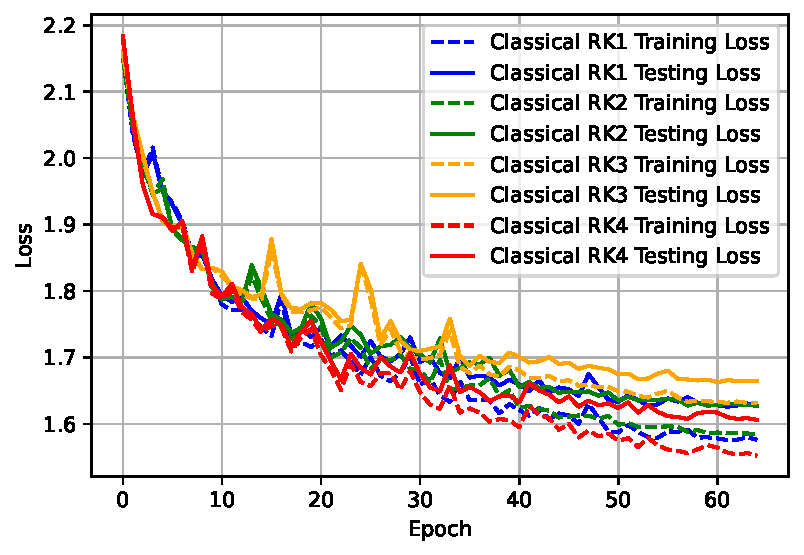
\includegraphics[scale=0.88]{./pics/new_pdf_graphs/classical/3_enc_1_rk_1_dec/classical_transfomer_loss_cifar10_rk1_rk2_rk3_rk4.pdf}
  \caption[Cross-entropy loss evolution during learning]{Cross-entropy loss evolution during learning}
  \label{fig:p29}
  \vspace*{\floatsep}
  \centering
  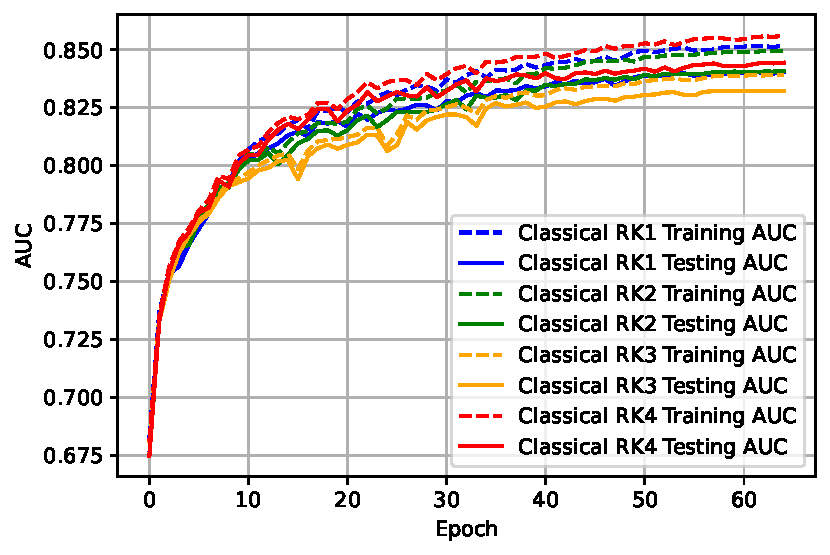
\includegraphics[scale=0.88]{./pics/new_pdf_graphs/classical/3_enc_1_rk_1_dec/classical_transfomer_auc_cifar10_rk1_rk2_rk3_rk4.pdf}
  \caption[AUC score evolution during learning]{AUC score evolution during learning}
  \label{fig:p30}
\end{figure}

This implementation showcases the following components and parameters:
\begin{itemize}
  \item \textbf{Patch Size}: 16
  \item \textbf{Hidden Size}: 12
  \item \textbf{Classical ODE-Transformer Blocks}: 1
  \item \textbf{Classical Attention Heads}: 6
  \item \textbf{Hidden MLP Size}: 6
\end{itemize}

\begin{table}[th]\small\linespread{1}
  \label{tab:classical_CIFAR_1}
  \centering
  \begin{tabular}{|l|c|c|c|c|c|c|}
    \hline
    \textbf{ODE} & \textbf{Train Time (s)} & \textbf{Accuracy} & \textbf{F1 Score} & \textbf{Best AUC Epoch} & \textbf{\# Parameters} & \textbf{\# Qubits} \\
    \hline
    RK1          & 1568.55                 & 41\%              & 41\%              & 62                      & 28894                  & -                  \\
    RK2          & 1521.45                 & 40\%              & 40\%              & 65                      & 29680                  & -                  \\
    RK3          & 1464.02                 & 38\%              & 38\%              & 61                      & 28084                  & -                  \\
    RK4          & 1685.04                 & 42\%              & 42\%              & 65                      & 33634                  & -                  \\
    \hline
  \end{tabular}
  \caption{CIFAR-10 metrics for the classical configurations}
\end{table}

Observations:

Training time varies slightly among the methods, with RK3 having the shortest training time and RK4 the longest.

The accuracy ranges from 38\% to 42\%, with RK4 achieving the highest accuracy.

The F1 score mirrors the accuracy, indicating a consistent balance between precision and recall across methods.

The best AUC epoch varies, with RK2 and RK4 achieving their peak performance later than RK1 and RK3.

The number of parameters increases with the order of the method, with RK4 having the most parameters.

\clearpage

And between the optimized RK4 and traditional RK4:

\begin{figure}[th]
  \centering
  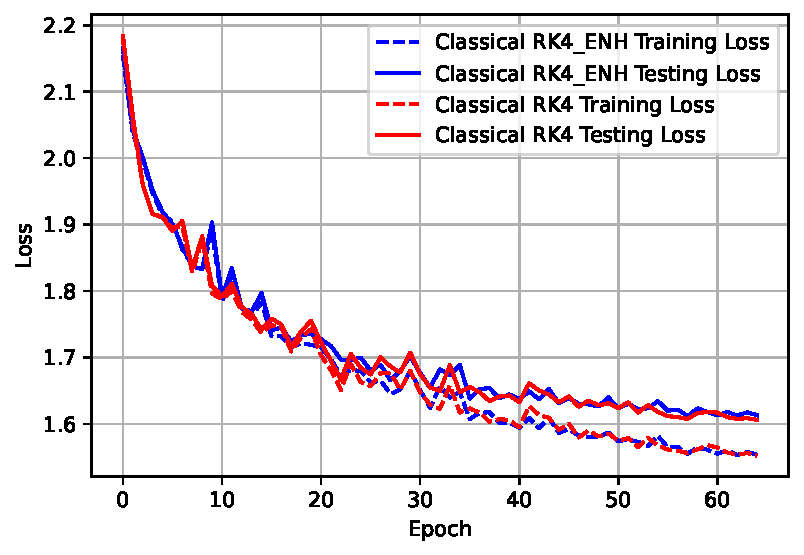
\includegraphics[scale=0.88]{./pics/new_pdf_graphs/classical/3_enc_1_rk_1_dec/classical_transfomer_loss_cifar10_rk4_rk4_enh.pdf}
  \caption[Cross-entropy loss evolution during learning]{Cross-entropy loss evolution during learning}
  \label{fig:p33}
  \vspace*{\floatsep}
  \centering
  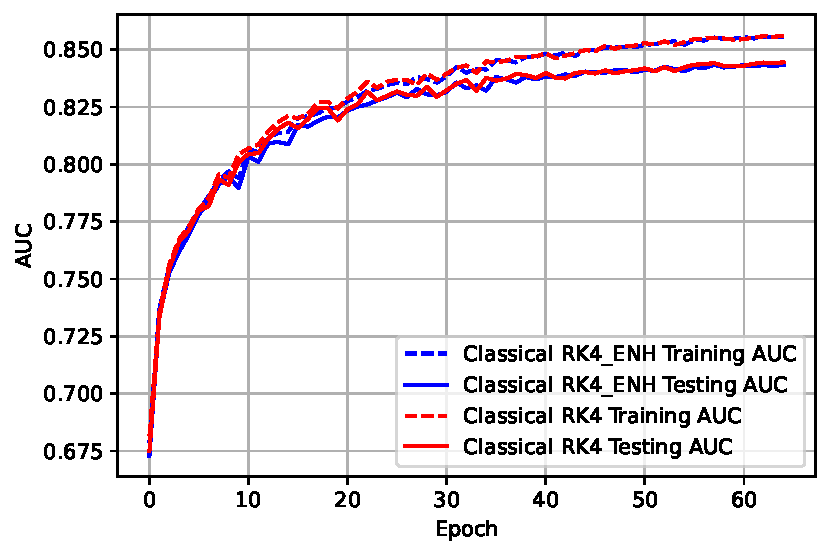
\includegraphics[scale=0.88]{./pics/new_pdf_graphs/classical/3_enc_1_rk_1_dec/classical_transfomer_auc_cifar10_rk4_rk4_enh.pdf}
  \caption[AUC score evolution during learning]{AUC score evolution during learning}
  \label{fig:p34}
\end{figure}

For the CIFAR-10 dataset, a more complex problem compared to MNIST, the optimized variant demonstrates noteworthy differences. Although it does not significantly improve training loss, testing loss, or AUC, it converges faster than the standard version. This optimized model requires fewer parameters and trains more quickly, showcasing efficiency gains. The increased complexity of CIFAR-10 means further adjustments have a more pronounced impact, but the inherent challenges of the dataset still limit substantial improvements in accuracy metrics. Nonetheless, the optimized version faster convergence and reduced parameter count highlight valuable advancements in model performance within this more intricate problem space.

\clearpage

\begin{table}[th]\small\linespread{1}
  \label{tab:classical_CIFAR_2}
  \centering
  \begin{tabular}{|l|c|c|c|c|c|c|}
    \hline
    \textbf{ODE} & \textbf{Train Time (s)} & \textbf{Accuracy} & \textbf{F1 Score} & \textbf{Best AUC Epoch} & \textbf{\# Parameters} & \textbf{\# Qubits} \\
    \hline
    RK4          & 1685.04                 & 42\%              & 42\%              & 65                      & 33634                  & -                  \\
    RK4\_ENH     & 1572.41                 & 41\%              & 41\%              & 58                      & 31252                  & -                  \\
    \hline
  \end{tabular}
  \caption{CIFAR-10 metrics for the classical configurations}
\end{table}

Observations:

The enhanced RK4 method has a reduced training time, suggesting improved computational efficiency.

The enhanced RK4 method shows a slight decrease in accuracy compared to the standard RK4 method.

The F1 score of the enhanced RK4 method is consistent with its accuracy, indicating a balanced precision and recall.

The enhanced RK4 method achieves its best AUC performance earlier, suggesting faster convergence.

The enhanced RK4 method has fewer parameters, indicating a reduction in model complexity.

\clearpage
The progress of the AUC and the loss using \textbf{one ODE quantum and classical blocks}-based network, calculated at every epoch, is here:

\begin{figure}[th]
  \centering
  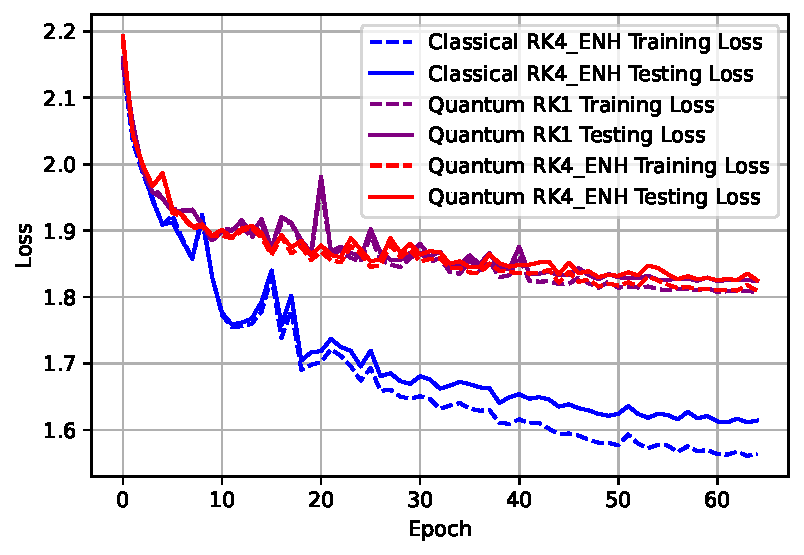
\includegraphics[scale=0.88]{./pics/new_pdf_graphs/hybrid/hybrid_transfomer_loss_cifar10_rk4_enh.pdf}
  \caption[Cross-entropy loss evolution during learning]{Cross-entropy loss evolution during learning}
  \label{fig:p35}
  \vspace*{\floatsep}
  \centering
  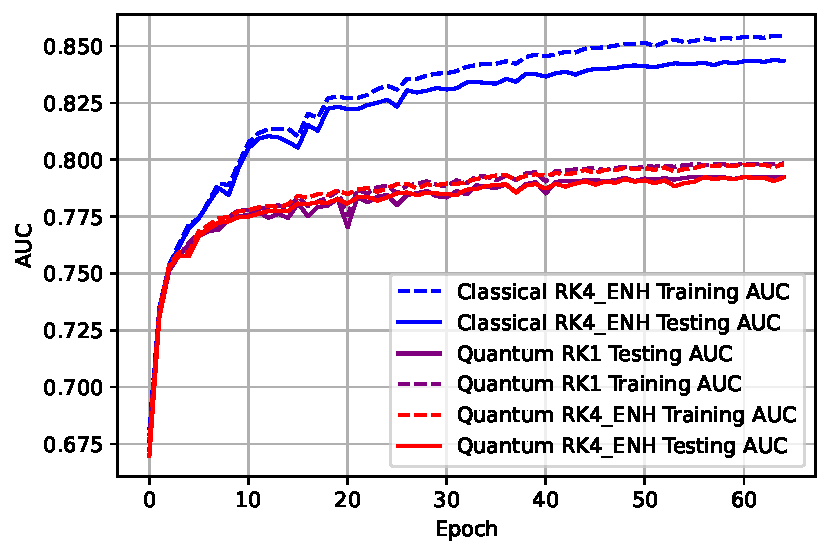
\includegraphics[scale=0.88]{./pics/new_pdf_graphs/hybrid/hybrid_auc_cifar10_.pdf}
  \caption[AUC score evolution during learning]{AUC score evolution during learning}
  \label{fig:p36}
\end{figure}

This implementation showcases the following components and parameters:
\begin{itemize}
  \item \textbf{Patch Size}: 16
  \item \textbf{Hidden Size}: 12
  \item \textbf{Classical and Quantum ODE-Transformer Blocks}: 1
  \item \textbf{Classical and Quantum Attention Heads}: 6
  \item \textbf{Hidden QMLP Size}: 6
\end{itemize}


\clearpage

\begin{table}[th]\small\linespread{1}
  \label{tab:hybrid_MNIST}
  \centering
  \begin{tabular}{|l|c|c|c|c|c|c|}
    \hline
    \textbf{ODE} & \textbf{Train Time (s)} & \textbf{Accuracy} & \textbf{F1 Score} & \textbf{Best AUC Epoch} & \textbf{\# Parameters} & \textbf{\# Qubits} \\
    \hline
    RK4\_ENH     & 1685.04                 & 42\%              & 42\%              & 65                      & 33634                  & -                  \\
    QRK4\_ENH    & 16724.79                & 34\%              & 33\%              & 61                      & 20590                  & 390                \\
    QRK1         & 10909.40                & 33\%              & 33\%              & 56                      & 20590                  & 336                \\
    \hline
  \end{tabular}
  \caption{CIFAR-10 metrics for the quantum and classical configurations}
\end{table}

Observations:

The training time for the enhanced quantum QRK4 method is significantly longer than the classical method. The training time for the first-order quantum RK method is shorter than QRK4\_ENH but still much longer than RK4\_ENH.

The accuracy of the enhanced quantum method is lower compared to the classical method. The first-order quantum RK method has slightly lower accuracy than the QRK4\_ENH method.

The F1 score of the first-order quantum RK method matches its accuracy, indicating balanced precision and recall.

The first-order quantum RK method achieves its best AUC performance the earliest among the methods listed.

The number of parameters is the same for both quantum methods.

The quantum methods require a significant number of qubits, highlighting the substantial quantum resources needed.

\clearpage

\section{IMDb Sentiment Analysis}

IMDb is a widely used dataset in Natural Language Processing, particularly for sentiment analysis tasks. It comprises 50,000 movie reviews, equally divided into 25,000 training reviews and 25,000 testing reviews. Each review is labeled as either positive or negative, providing a binary classification challenge. The dataset complexity arises from the nuances of human language, including sarcasm, idioms, and varying lengths of reviews, making it an excellent benchmark for evaluating advanced sentiment analysis models.

In this experiment, the IMDb dataset is meticulously divided into three distinct segments to ensure thorough model evaluation and optimization. The training split, comprising 22,500 reviews, provides a robust foundation for the model to learn diverse linguistic patterns and sentiment cues. A validation split of 2,500 reviews is utilized during the Random Search process for hyperparameter tuning and model refinement, enabling the selection of the best-performing model configuration. Finally, to rigorously assess the model generalization capability, 25,000 reviews are reserved in the test set, remaining unseen during the training phase. This method ensures that the model is not only well-trained but also demonstrates effective performance on new, unseen data, accurately reflecting its true predictive power in sentiment analysis tasks.

Some extracted samples are shown below:

\begin{table}[h!]
  \centering
  \begin{tabular}{|c|p{12cm}|}
    \hline
    \textbf{Label} & \textbf{Text}                                                                                                                                                                                                                                                                                                                                                                                                                                                                                                                                                                                                                                                                                                                                                                             \\
    \hline
    0 (neg)        & "I have been known to fall asleep during films, but this is usually due to a combination of things including, really tired, being warm and comfortable on the settee and having just eaten a lot. However on this occasion I fell asleep because the film was rubbish. The plot development was constant. Constantly slow and boring. Things seemed to happen, but with no explanation of what was causing them or why. I admit, I may have missed part of the film, but I watched the majority of it and everything just seemed to happen of its own accord without any real concern for anything else. I can't recommend this film at all."                                                                                                                                             \\
    \hline
    1 (pos)        & "This is a film which should be seen by anybody interested in, effected by, or suffering from an eating disorder. It is an amazingly accurate and sensitive portrayal of bulimia in a teenage girl, its causes and its symptoms. The girl is played by one of the most brilliant young actresses working in cinema today, Alison Lohman, who was later so spectacular in 'Where the Truth Lies'. I would recommend that this film be shown in all schools, as you will never see a better on this subject. Alison Lohman is absolutely outstanding, and one marvels at her ability to convey the anguish of a girl suffering from this compulsive disorder. If barometers tell us the air pressure, Alison Lohman tells us the emotional pressure with the same degree of accuracy [...]" \\
    \hline
  \end{tabular}
  \caption{Movie Reviews\protect\footnotemark}
  \label{table:negative_reviews}
\end{table}\footnotetext{https://www.tensorflow.org/datasets/catalog/imdb\_reviews}

\clearpage

The progress of the AUC and the loss using \textbf{one classical ODE block}-based network, calculated at every epoch, is here:

\begin{figure}[th]
  \centering
  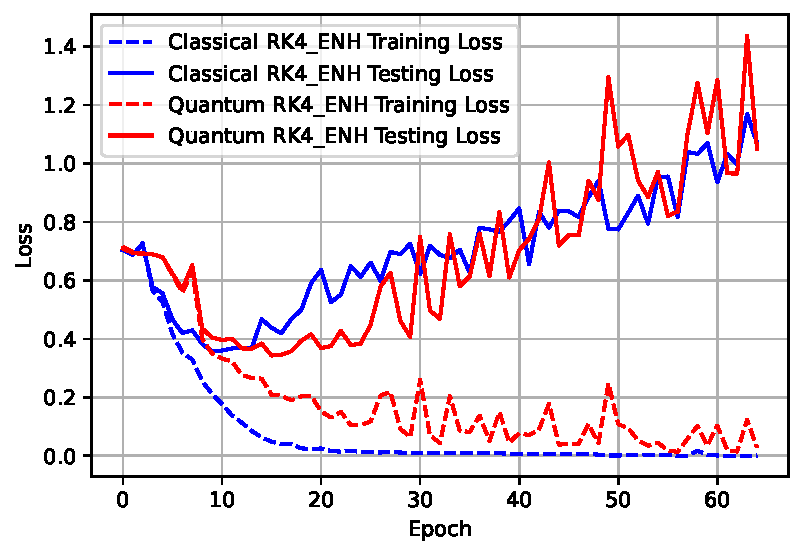
\includegraphics[scale=0.88]{./pics/new_pdf_graphs/hybrid/hybrid_transfomer_loss_imdb_rk4_enh.pdf}
  \caption[Cross-entropy loss evolution during learning]{Cross-entropy loss evolution during learning}
  \label{fig:p37}
  \vspace*{\floatsep}
  \centering
  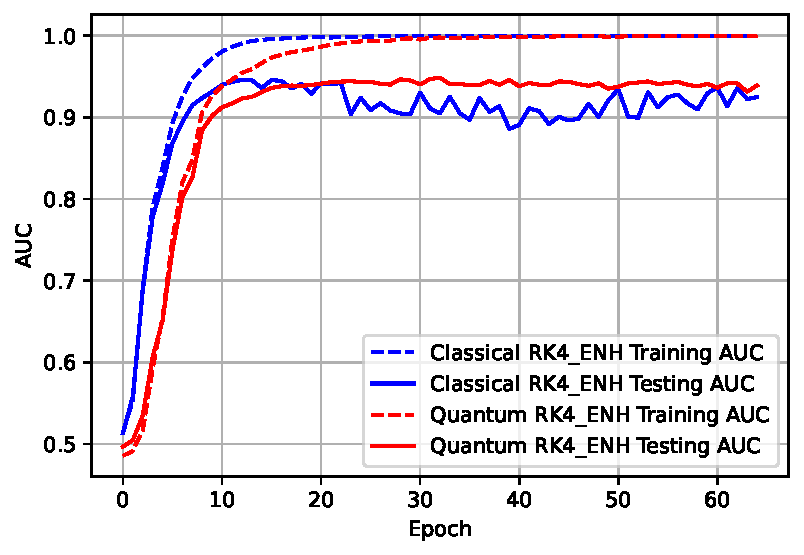
\includegraphics[scale=0.88]{./pics/new_pdf_graphs/hybrid/hybrid_auc_imdb_.pdf}
  \caption[AUC score evolution during learning]{AUC score evolution during learning}
  \label{fig:p38}
\end{figure}

This implementation showcases the following components and parameters:
\begin{itemize}
  \item \textbf{Max sequence length}: 512
  \item \textbf{Classical / Quantum Hidden Size}: 12 / 6
  \item \textbf{Classical / Quantum ODE-Transformer Blocks}: 1 / 1
  \item \textbf{Classical / Quantum Attention Heads}: 6 / 2
  \item \textbf{Classical / Quantum Hidden MLP Size}: 6 / 4
\end{itemize}

\begin{table}[th]\small\linespread{1}
  \label{tab:classical_CIFAR_1}
  \centering
  \begin{tabular}{|l|c|c|c|c|c|c|}
    \hline
    \textbf{ODE} & \textbf{Train Time (s)} & \textbf{Accuracy} & \textbf{F1 Score} & \textbf{Best AUC Epoch} & \textbf{\# Parameters} & \textbf{\# Qubits} \\
    \hline
    RK4\_ENH     & 3328.61                 & 85\%              & 85\%              & 13                      & 499316                 & -                  \\
    QRK4\_ENH    & 9033.13                 & \textbf{85}\%     & \textbf{85}\%     & 33                      & \textbf{243896}        & 141                \\
    \hline
  \end{tabular}
  \caption{IMDb metrics for the classical and quantum configurations}
\end{table}

The quantum-enhanced configuration (QRK4\_ENH) takes significantly longer to train, almost three times as long as the classical configuration (RK4\_ENH). This suggests that while quantum methods may have computational benefits, they currently require more training time, possibly due to the complexity of quantum computations and the need for more iterations to converge.

Despite the increased training time for the quantum-enhanced model, it does not result in higher accuracy or F1 score compared to the classical model. This indicates that the quantum enhancement does not compromise the model performance on these metrics.

The best epoch for the Area Under the Curve (AUC) metric occurs earlier for the classical configuration compared to the quantum-enhanced one. This could imply that the classical model reaches its optimal performance faster during training, whereas the quantum-enhanced model requires more epochs to achieve its best performance.

The quantum-enhanced configuration has approximately 51\% fewer parameters than the classical configuration. This significant reduction in the number of parameters is a crucial observation, as it highlights the potential of quantum methods in optimizing model complexity and reducing resource requirements without sacrificing performance.

\clearpage

\section{QRKT-GAN and TransGAN Synthetic Data Generation}

This section provides a detailed comparison of the synthetic data generation capabilities of two distinct Generative Adversarial Networks (GANs): TransGAN and QRKT-GAN. While both aim to generate high-quality images, their underlying architectures and training processes differ significantly.

The training hyperparameters for both GANs are summarized as follows~\cite{ahmet_sarigun_2024_10806360}:

\begin{itemize}
  \item Learning Rate for Discriminator: 0.0001
  \item Learning Rate for Generator: 0.0001
  \item Latent Dimension: 1024
  \item Batch Size for Generator: 32
  \item Batch Size for Discriminator: 32
  \item Number of Epochs: 40
  \item Weight Decay: 1e-3
  \item Dropout Rate: 0.5
  \item Number of Critic Steps: 5
  \item Maximum Iterations: 500000
  \item Learning Rate Decay: True
\end{itemize}

The architectural details are as follows:

\begin{itemize}
  \item Image Size: 32
  \item Initial Size: 8
  \item Patch Size: 4
  \item Embedding Dimension: 384
  \item Optimizer: 'Adam'
  \item Loss Function: "wgangp\_eps"
  \item Phi: 1
  \item Beta1: 0
  \item Beta2: 0.99
  \item Data Augmentation: True
\end{itemize}

Due to high computational limitations, QRKT-GAN has weaker architectural components for both the Generator and Discriminator. QRKT-GAN was trained for only 40 epochs, owing to the very high generation time and VRAM consumption for this quantum model. The training utilized the Nvidia A100-PCIE-40GB GPU from the cluster. For QRKT-GAN, the data augmentation techniques specified were applied to mitigate some of these limitations.

However, the ODE-based Transformer block using optimized RK4 could be applied to the Generator network, further enhancing the quality of images and the obtained scores.

The Discriminator, unfortunately, doesn't have any ODE blocks in its composition due to high memory consumption during training. It exclusively employs Encoders integrated with Variational Quantum Circuits (VQCs). QRKT-GAN uses 384 qubits.

The performance metrics for QRKT-GAN and TransGAN are summarized in the table below:

\begin{table}[h!]
  \centering
  \begin{tabular}{|c|c|c|}
    \hline
    \textbf{Metric}                  & \textbf{QRKT-GAN} & \textbf{TransGAN} \\
    \hline
    Inception Score (IS)             & 74.89             & 52.31             \\
    \hline
    Fréchet Inception Distance (FID) & 66.78             & 46.97             \\
    \hline
  \end{tabular}
  \caption{Performance Metrics for TransGAN and QRKT-GAN on CIFAR-10 using 40 epochs}
  \label{table:performance_metrics}
\end{table}

\begin{figure}[th]
  \centering
  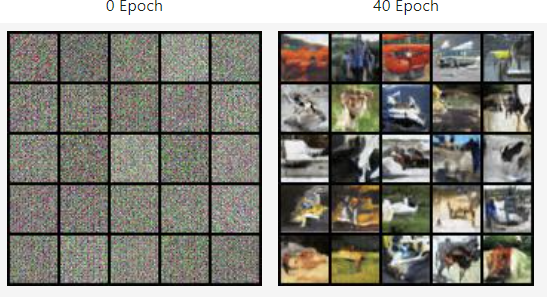
\includegraphics[scale=0.7]{./pics/gan_gen.png}
  \caption[Generated Images using TransGAN]{Generated Images using TransGAN~\cite{ahmet_sarigun_2024_10806360}}
  \label{fig:p40}
\end{figure}

\begin{figure}[th]
  \centering
  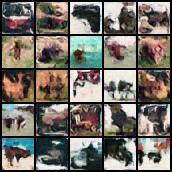
\includegraphics[scale=0.88]{./pics/generated_img_39_1600.jpg}
  \caption[Generated Images using QRKT-GAN]{Generated Images using QRKT-GAN}
  \label{fig:p41}
\end{figure}

Future investigations are numerous and essential to advancing the field. One crucial area is the development of fault-tolerant quantum hardware, which would allow for more reliable and scalable implementations of quantum GANs. Additionally, testing QRKT-GAN on various quantum architectures, including those based on trapped ions, superconducting qubits, and photonic systems, could provide deeper insights into the most effective configurations.

Further research should also explore the use of Quantum Graph Networks (QGNs) and Quantum Random Walks for optimizing network-based models. Quantum Annealing, particularly for combinatorial optimization problems, presents another promising avenue for enhancing GAN performance.

While QRKT-GAN currently faces significant limitations, ongoing advancements in Quantum Computing hardware and algorithms hold the promise of achieving Quantum Artificial Intelligence that can surpass classical methods in generating high-quality synthetic data.

\chapter{Conclusions and Future Work}\vspace{-12pt}
The comprehensive experiments and theoretical discussions presented in this thesis underscore the transformative potential of Quantum Computing in optimizing Deep Learning models. These results reveal that quantum techniques can significantly reduce the number of trainable parameters, thereby decreasing the energy consumption required for training such models. This is particularly crucial in domains where computational resources and energy efficiency are critical constraints.

The research primarily focused on Variational Quantum Circuits (VQCs) and Variational Quantum Algorithms (VQAs), illustrating their capacity to compress neural networks without compromising performance. These quantum methodologies offer a promising alternative to traditional Deep Learning optimization techniques, especially in scenarios demanding high efficiency and lower energy footprints.

However, the journey of integrating Quantum Computing with Artificial Intelligence is just beginning, and there are numerous avenues for future research and exploration. A pivotal area for future investigation is the development and implementation of fault-tolerant quantum hardware. The current generation of quantum devices is plagued by high error rates and issues related to decoherence, which limit their practical applications. Achieving fault tolerance in quantum hardware will be a significant milestone, enabling more reliable and extensive testing of quantum-enhanced AI models on real-world tasks.

Beyond improving hardware, future research should focus on testing these quantum models on diverse quantum architectures. Different quantum computing paradigms, such as those based on trapped ions, superconducting qubits, and photonic systems, offer unique advantages and challenges. Exploring these architectures will provide a more comprehensive understanding of how quantum computing can be leveraged to enhance AI.

Moreover, future work should include extensive benchmarking and testing of VQCs and VQAs on practical, real-world problems. This involves assessing their scalability, robustness, and generalizability across different domains. By conducting these tests, researchers can validate the practical utility of quantum-enhanced AI models and identify any limitations that need to be addressed.

Based on the insights and experimental results presented in this thesis, it is evident that Quantum Computing is poised to play a pivotal role in the future of Artificial Intelligence. The integration of quantum mechanics and AI could give rise to a stronger Quantum Artificial Intelligence, a new paradigm that leverages the unique properties of quantum systems to achieve capabilities beyond those of classical AI. This future holds the promise of more efficient, powerful, and intelligent systems capable of solving complex problems that are currently intractable.

In summary, while significant challenges remain, the potential for Quantum Computing to revolutionize AI is immense. Continued research and development in this area are essential to realize the full potential of Quantum Artificial Intelligence. By exploring diverse quantum architectures, advanced quantum techniques, and practical applications, it can be ensured that Quantum Computing becomes a cornerstone of future advancements in Artificial Intelligence.
\chapter{Bibliography}

\bibliographystyle{unsrt}

\begingroup
\def\chapter*#1{}
\bibliography{bibliography}
\endgroup

\end{document}
